% !TEX root = ../supplementary.tex
\renewcommand{\thefigure}{S\arabic{figure}}
\renewcommand{\thetable}{S\arabic{table}}
\renewcommand{\theHfigure}{S\arabic{figure}}
\renewcommand{\theHtable}{S\arabic{table}}
\setcounter{figure}{0}
\setcounter{table}{0}
\section*{Supplementary Results}

\subsection*{Baseline methodological controls}

The baseline simulations remain necessary controls for the extension. They establish the gold-standard power curve, expose inflation from selecting and testing a topology on the same alignment, show the benefit and possible conservatism of taxon-pair Bonferroni correction, and document the distinct effect of substitution-model misspecification. The newly generated JC, GTR, protein and misspecification panels below reproduce these methodological comparisons using the current implementation and verified publication grids; no artwork from the earlier paper is reused.

\begin{table}[p]
  \centering
  \small
  \begin{tabular}{llrrrr}
    \toprule
    Model & Sites & Branch \(t\) & Counterfactual & Refined & Difference \\
    \midrule
    \(+I+G4\) & 100 & 50 & 0.100 & 0.115 & 0.015 \\
     & 500 & 40 & 0.342 & 0.384 & 0.042 \\
     & 1,000 & 45 & 0.406 & 0.456 & 0.050 \\
     & 5,000 & 60 & 0.482 & 0.584 & 0.102 \\
     & 10,000 & 60 & 0.718 & 0.835 & 0.116 \\
    \addlinespace
    \(+I+R4\) & 100 & 10 & 0.558 & 0.573 & 0.015 \\
     & 500 & 20 & 0.405 & 0.450 & 0.044 \\
     & 1,000 & 22.5 & 0.449 & 0.522 & 0.073 \\
     & 5,000 & 30 & 0.501 & 0.605 & 0.104 \\
     & 10,000 & 35 & 0.402 & 0.565 & 0.163 \\
    \bottomrule
  \end{tabular}
  \caption{\textbf{Largest calibrated power gain at each alignment length in the invariant-mixture grid.} Differences are refined minus counterfactual; both formulas evaluate every alignment.}
\end{table}

\begin{figure}[p]
  \centering
  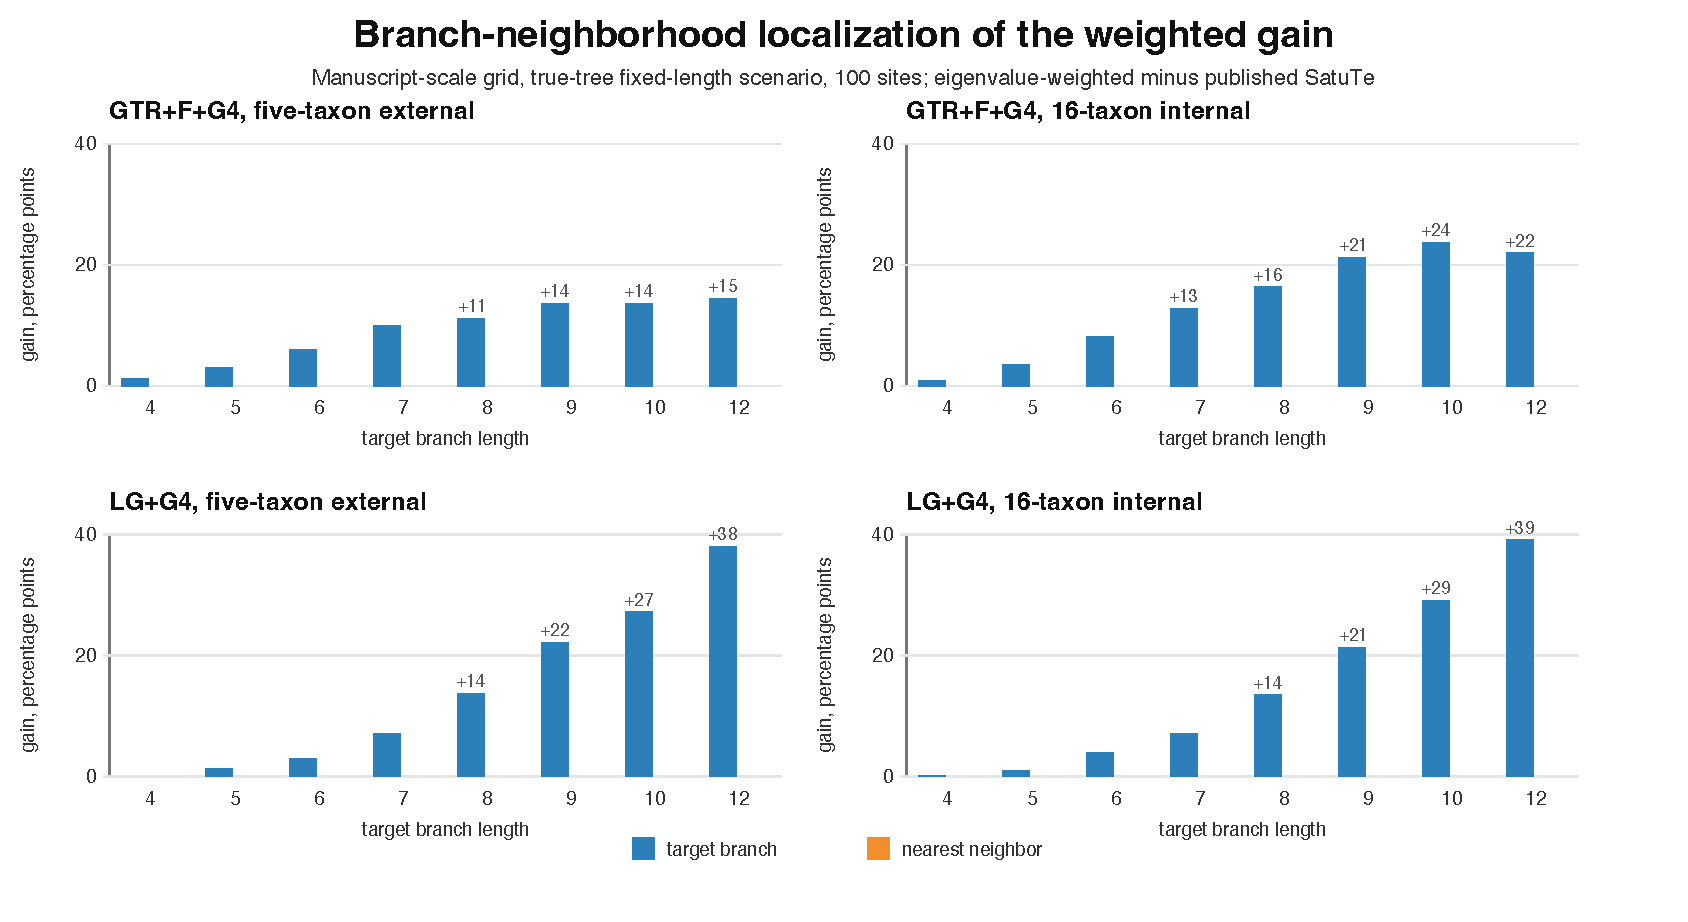
\includegraphics[width=0.98\textwidth]{figures/figure_branch_localization_compact.pdf}
  \caption{\textbf{Branch-neighbourhood localization.} Weighted-minus-dominant changes in informative-call fraction for the tested branch and adjacent branches. The change is concentrated on the deliberately lengthened focal branch.}
\end{figure}

\begin{figure}[p]
  \centering
  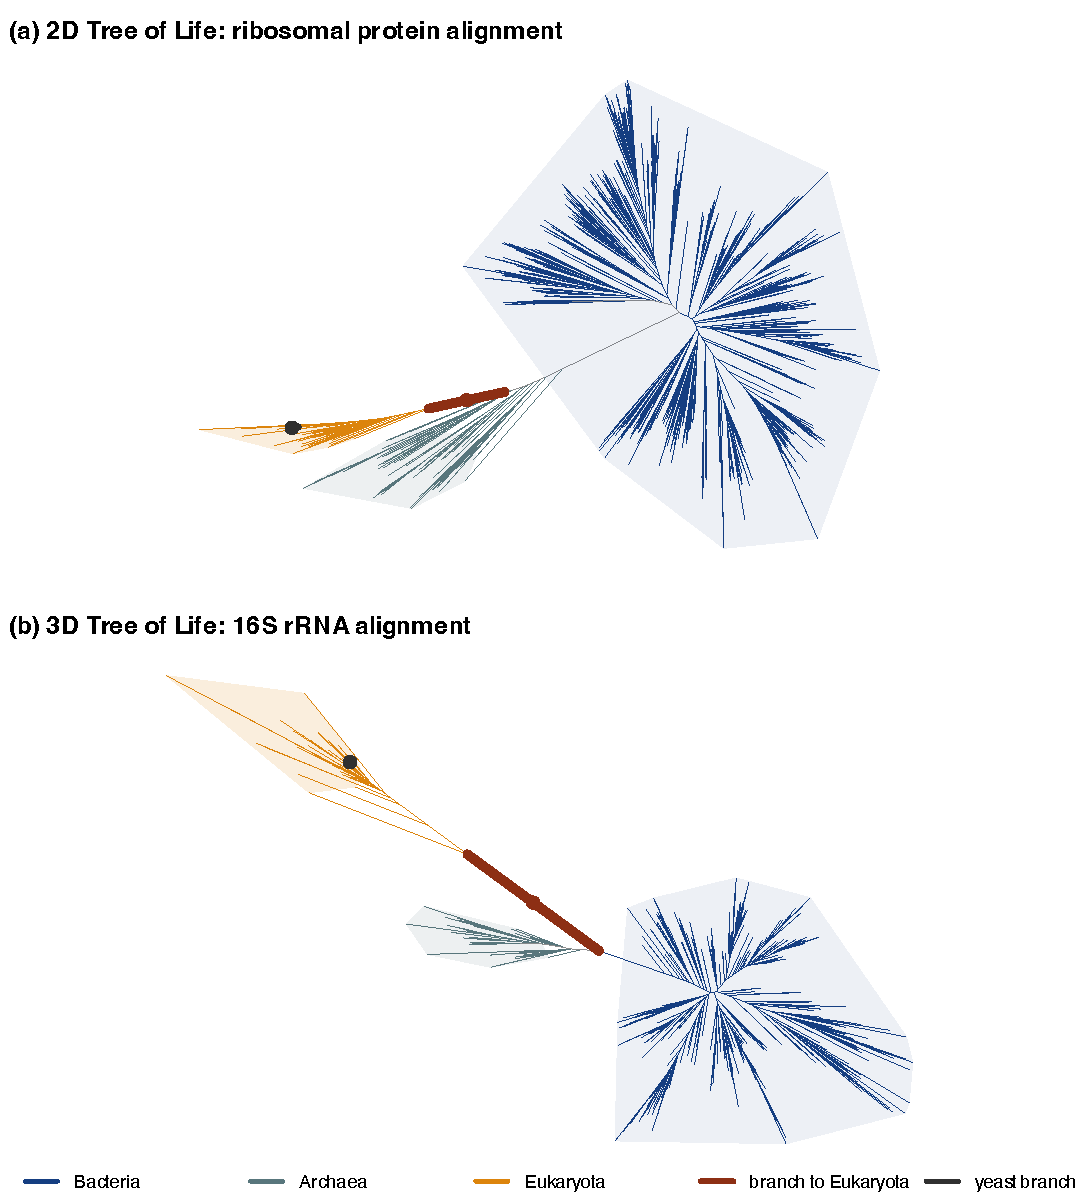
\includegraphics[width=0.88\textwidth]{figures/figure_tree_of_life_reference.pdf}
  \caption{\textbf{Tree-of-Life reference trees.} \textbf{a,} Ribosomal-protein 2D tree. \textbf{b,} 16S rRNA 3D tree. Colors and hulls identify Bacteria, Archaea and Eukaryota. The highlighted internal segment marks the branch leading to Eukaryota; the black marker identifies the yeast branch.}
\end{figure}

\begin{figure}[p]
  \centering
  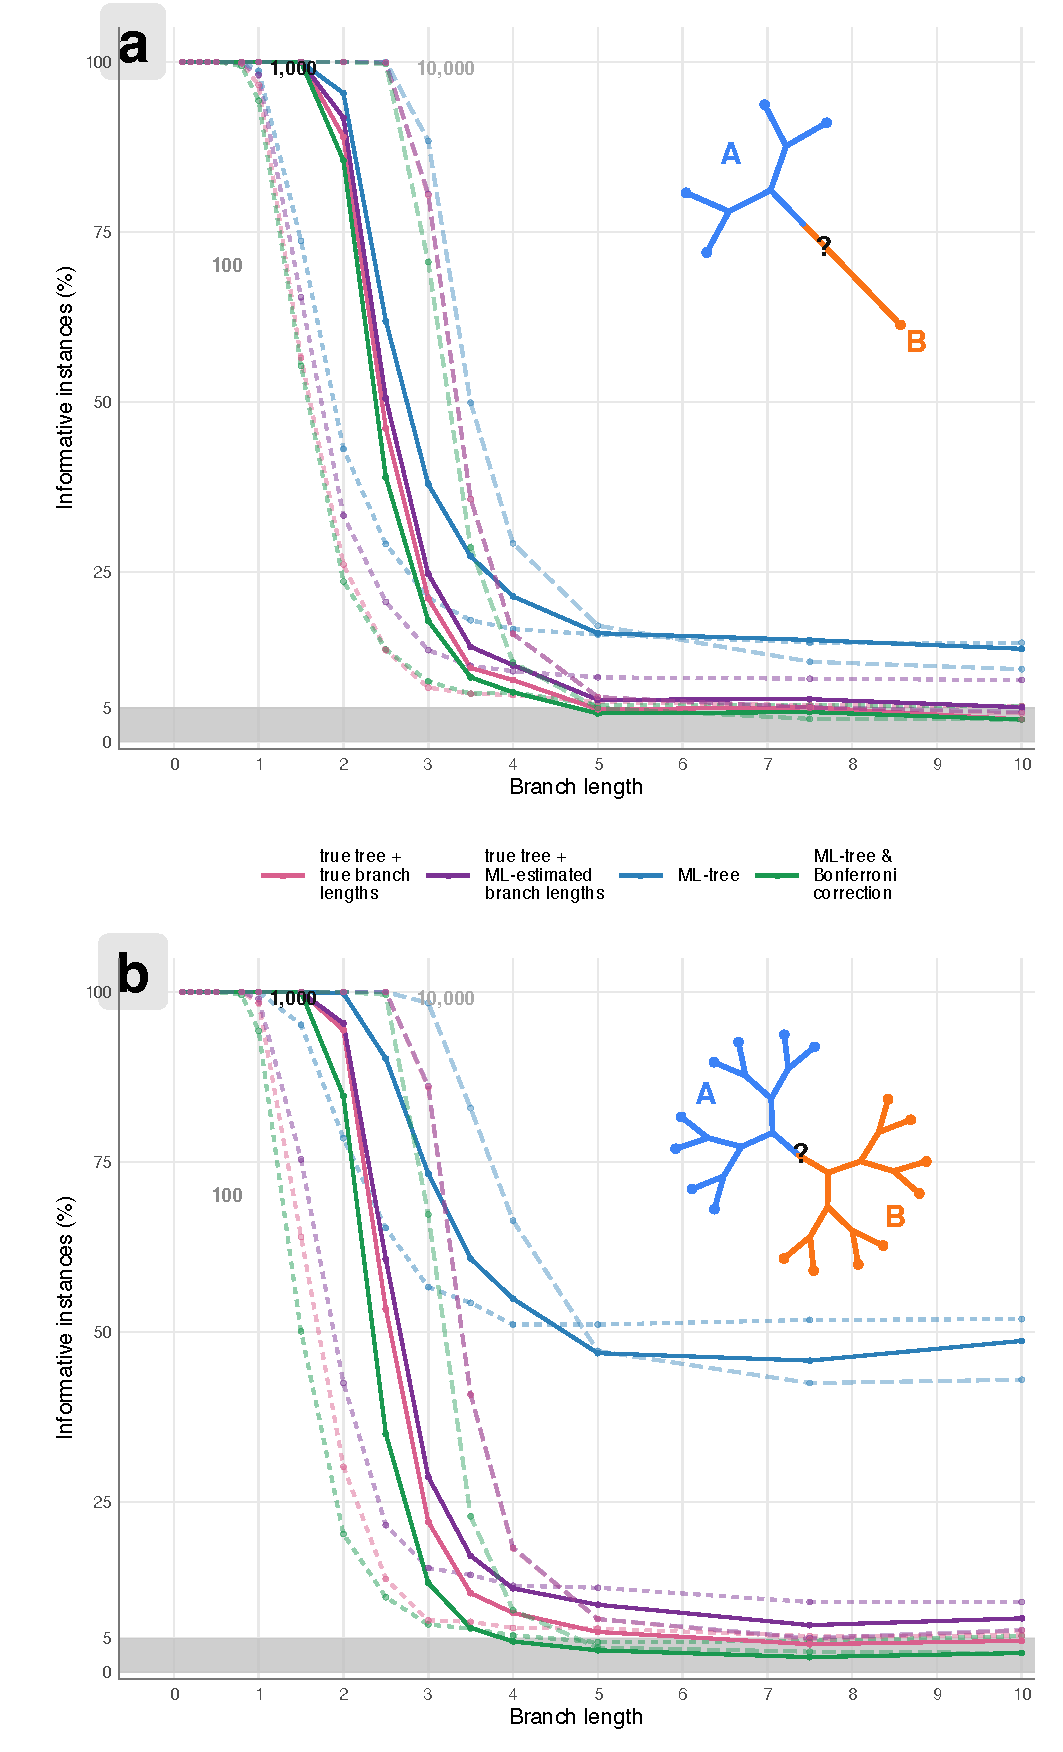
\includegraphics[width=0.98\textwidth]{figures/figure_jc_baseline_power.pdf}
  \caption{\textbf{Direct comparison with the original SatuTe simulation design.} The current implementation repeats the original paper's JC grid for five-taxon external and 16-taxon internal targets. Colors distinguish the true-tree reference, maximum-likelihood branch-length estimation, reuse of the alignment for topology selection and testing, and taxon-pair Bonferroni correction. Line styles show 100, 1,000 and 10,000 sites; every point contains 1,000 replicates.}
\end{figure}

\begin{figure}[p]
  \centering
  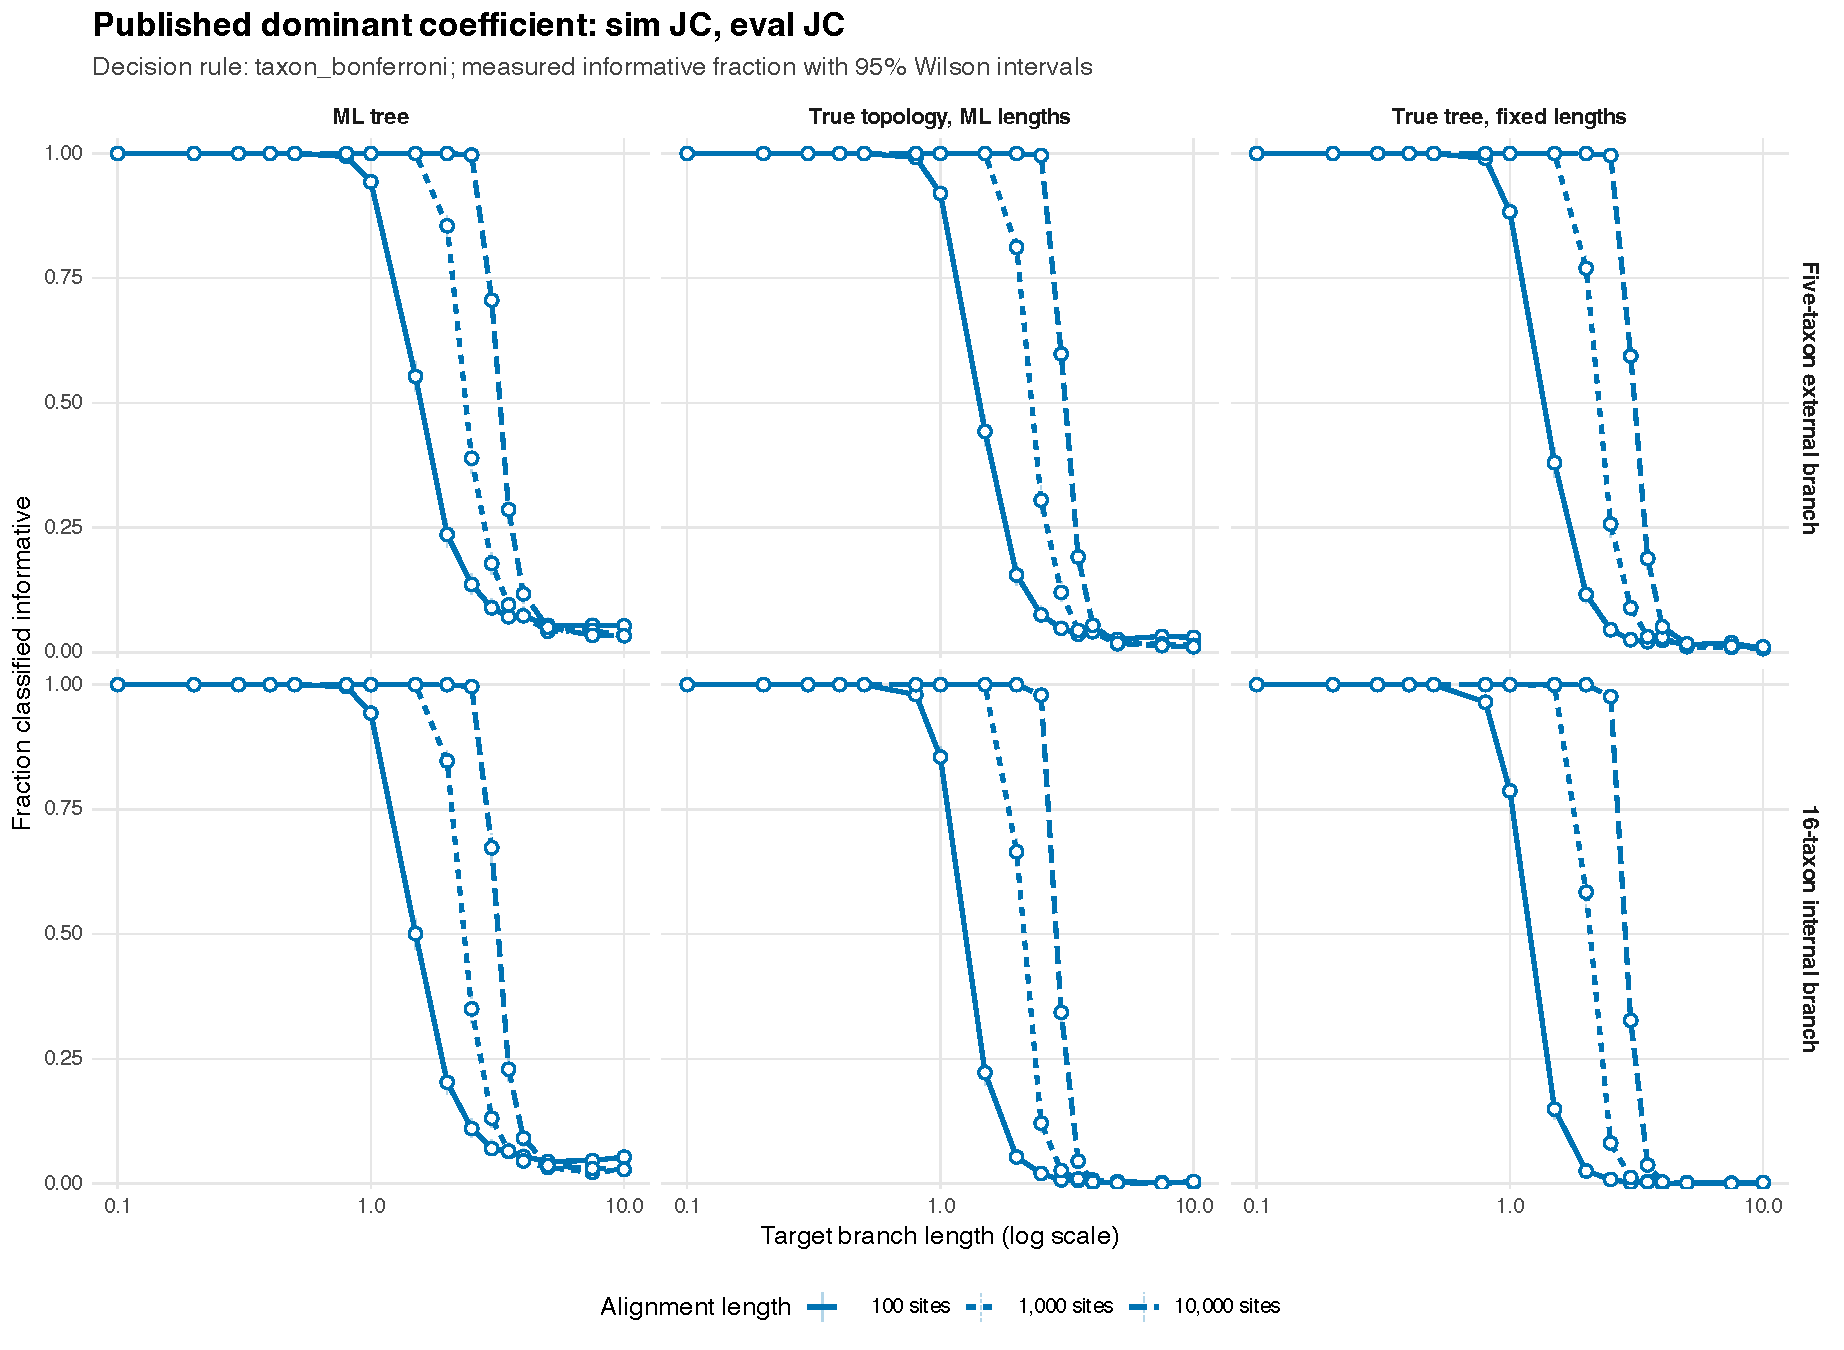
\includegraphics[width=0.49\textwidth]{figures/publication-suite/power/jc_JC_dominant.pdf}
  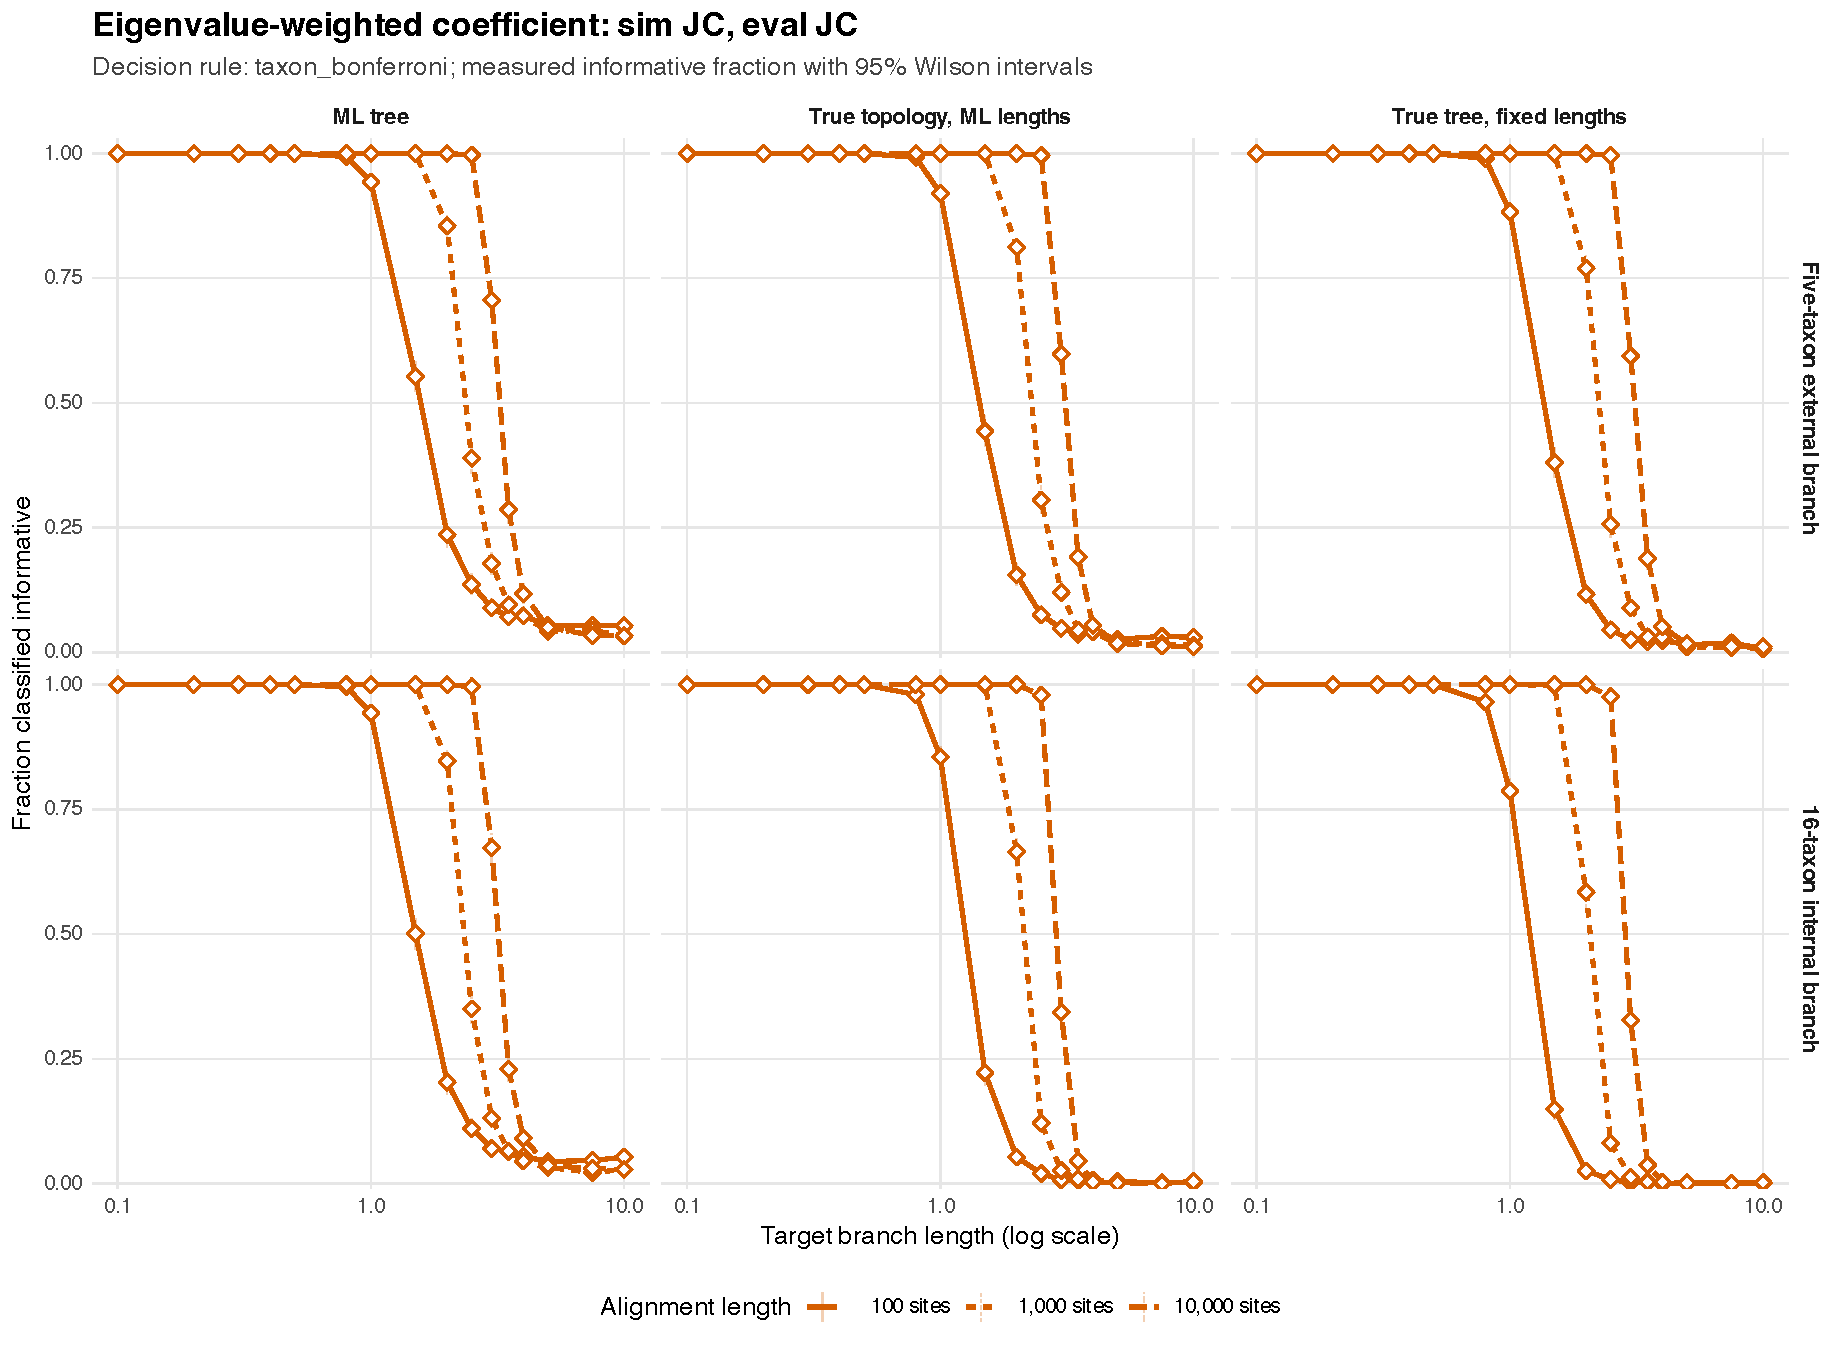
\includegraphics[width=0.49\textwidth]{figures/publication-suite/power/jc_JC_weighted.pdf}
  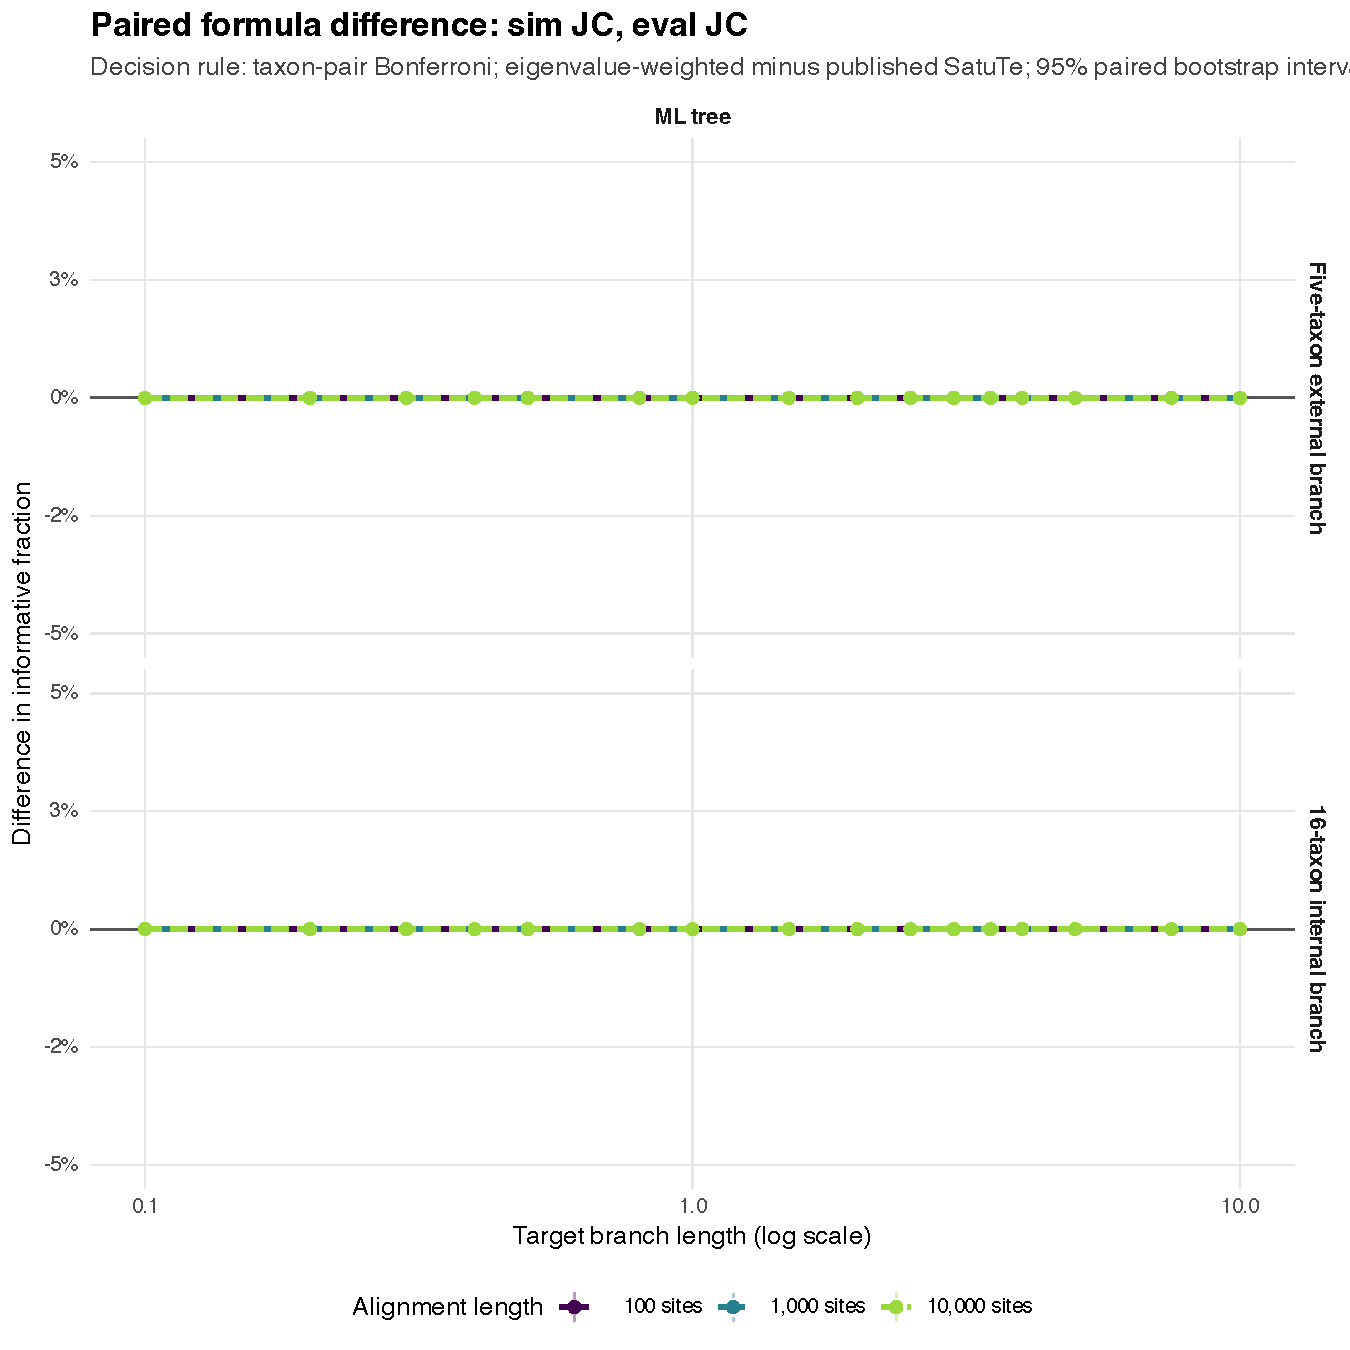
\includegraphics[width=0.72\textwidth]{figures/publication-suite/power/jc_JC_difference.pdf}
  \caption{\textbf{JC power in the common comparison layout.} Dominant (top left), eigenvalue-weighted (top right) and paired difference (bottom) under taxon Bonferroni. The two formulas are identical under JC, so the paired difference is exactly zero in all 288 design cells.}
\end{figure}

\subsection*{Topology-selection and bootstrap controls}

\begin{table}[p]
  \centering
  \small
  \begin{tabular}{rrrrrrrrrr}
    \toprule
    & \multicolumn{3}{c}{Two external attachments} & \multicolumn{3}{c}{One external attachment} & \multicolumn{3}{c}{Correct topology (\%)} \\
    \cmidrule(lr){2-4}\cmidrule(lr){5-7}\cmidrule(lr){8-10}
    \(t\) & 100 & 1,000 & 10,000 & 100 & 1,000 & 10,000 & 100 & 1,000 & 10,000 \\
    \midrule
    0.1 & 0 & 0 & 0 & 10 & 0 & 0 & 63.2 & 100.0 & 100.0 \\
    0.5 & 29 & 0 & 0 & 201 & 0 & 0 & 29.0 & 99.3 & 100.0 \\
    1.0 & 317 & 0 & 0 & 442 & 9 & 0 & 4.5 & 82.5 & 100.0 \\
    2.0 & 736 & 386 & 1 & 238 & 427 & 22 & 0.1 & 4.3 & 74.4 \\
    3.0 & 783 & 697 & 378 & 206 & 279 & 475 & 0.0 & 0.3 & 3.2 \\
    5.0 & 834 & 776 & 699 & 160 & 211 & 291 & 0.0 & 0.0 & 0.0 \\
    10.0 & 828 & 809 & 722 & 162 & 182 & 270 & 0.0 & 0.0 & 0.0 \\
    \bottomrule
  \end{tabular}
  \caption{\textbf{Representative split-placement results.} Counts among 1,000 inferred 16-taxon ML trees in which the branch separating the two eight-taxon subtrees attaches two external branches or one external and one internal branch, together with full-topology reconstruction accuracy. The omitted intermediate branch lengths follow the same monotone deterioration reported in the baseline experiment. Columns are alignment lengths in sites.}
  \makeatletter\cref@old@label{tab-supp-placement}\makeatother
\end{table}

\begin{table}[p]
  \centering
  \small
  \begin{tabular}{rrrrr}
    \toprule
    Focal \(t\) & Split present & Mean bootstrap & Minimum bootstrap & SatuTe informative (\%) \\
    \midrule
    0.1 & 993 & 93.32 & 14 & 100.0 \\
    0.2 & 999 & 99.19 & 74 & 100.0 \\
    0.5 & 1,000 & 99.99 & 97 & 100.0 \\
    0.8 & 1,000 & 100.00 & 100 & 99.1 \\
    1.0 & 1,000 & 100.00 & 100 & 92.4 \\
    1.5 & 1,000 & 100.00 & 100 & 49.7 \\
    2.0 & 1,000 & 100.00 & 100 & 21.6 \\
    2.5 & 1,000 & 100.00 & 100 & 9.6 \\
    3.0 & 1,000 & 100.00 & 100 & 5.9 \\
    3.5 & 1,000 & 100.00 & 100 & 4.3 \\
    4.0 & 1,000 & 100.00 & 100 & 4.6 \\
    5.0 & 1,000 & 100.00 & 100 & 3.8 \\
    7.5 & 1,000 & 100.00 & 100 & 3.5 \\
    10.0 & 1,000 & 100.00 & 100 & 4.3 \\
    \bottomrule
  \end{tabular}
  \caption{\textbf{Bootstrap--saturation contrast.} For 1,000 JC alignments of 100 sites on the 16-taxon tree, bootstrap support for the inferred split remains perfect at long focal branches while the Bonferroni SatuTe informative fraction approaches the 5\% null level. This is the empirical basis for treating SatuTe as complementary to bootstrap support.}
  \makeatletter\cref@old@label{tab-supp-bootstrap}\makeatother
\end{table}

\clearpage

\begin{figure}[p]
  \centering
  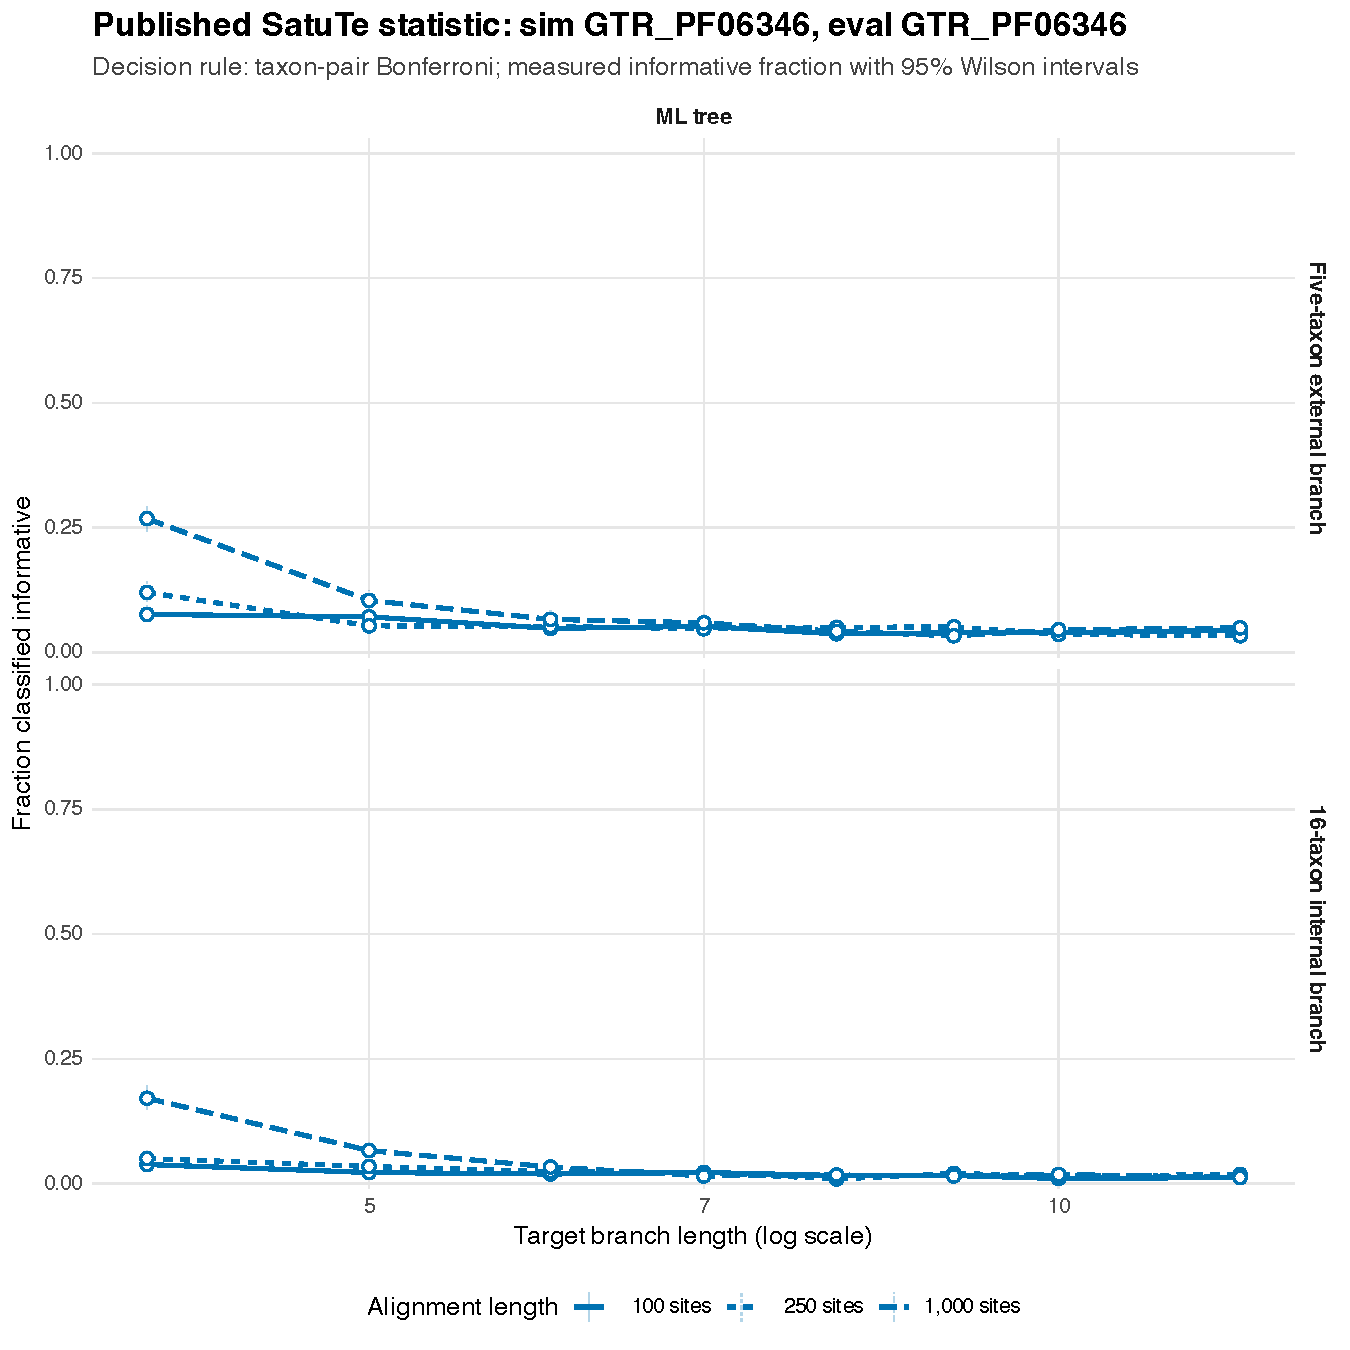
\includegraphics[width=0.49\textwidth]{figures/publication-suite/power/gtr_GTR_PF06346_dominant.pdf}
  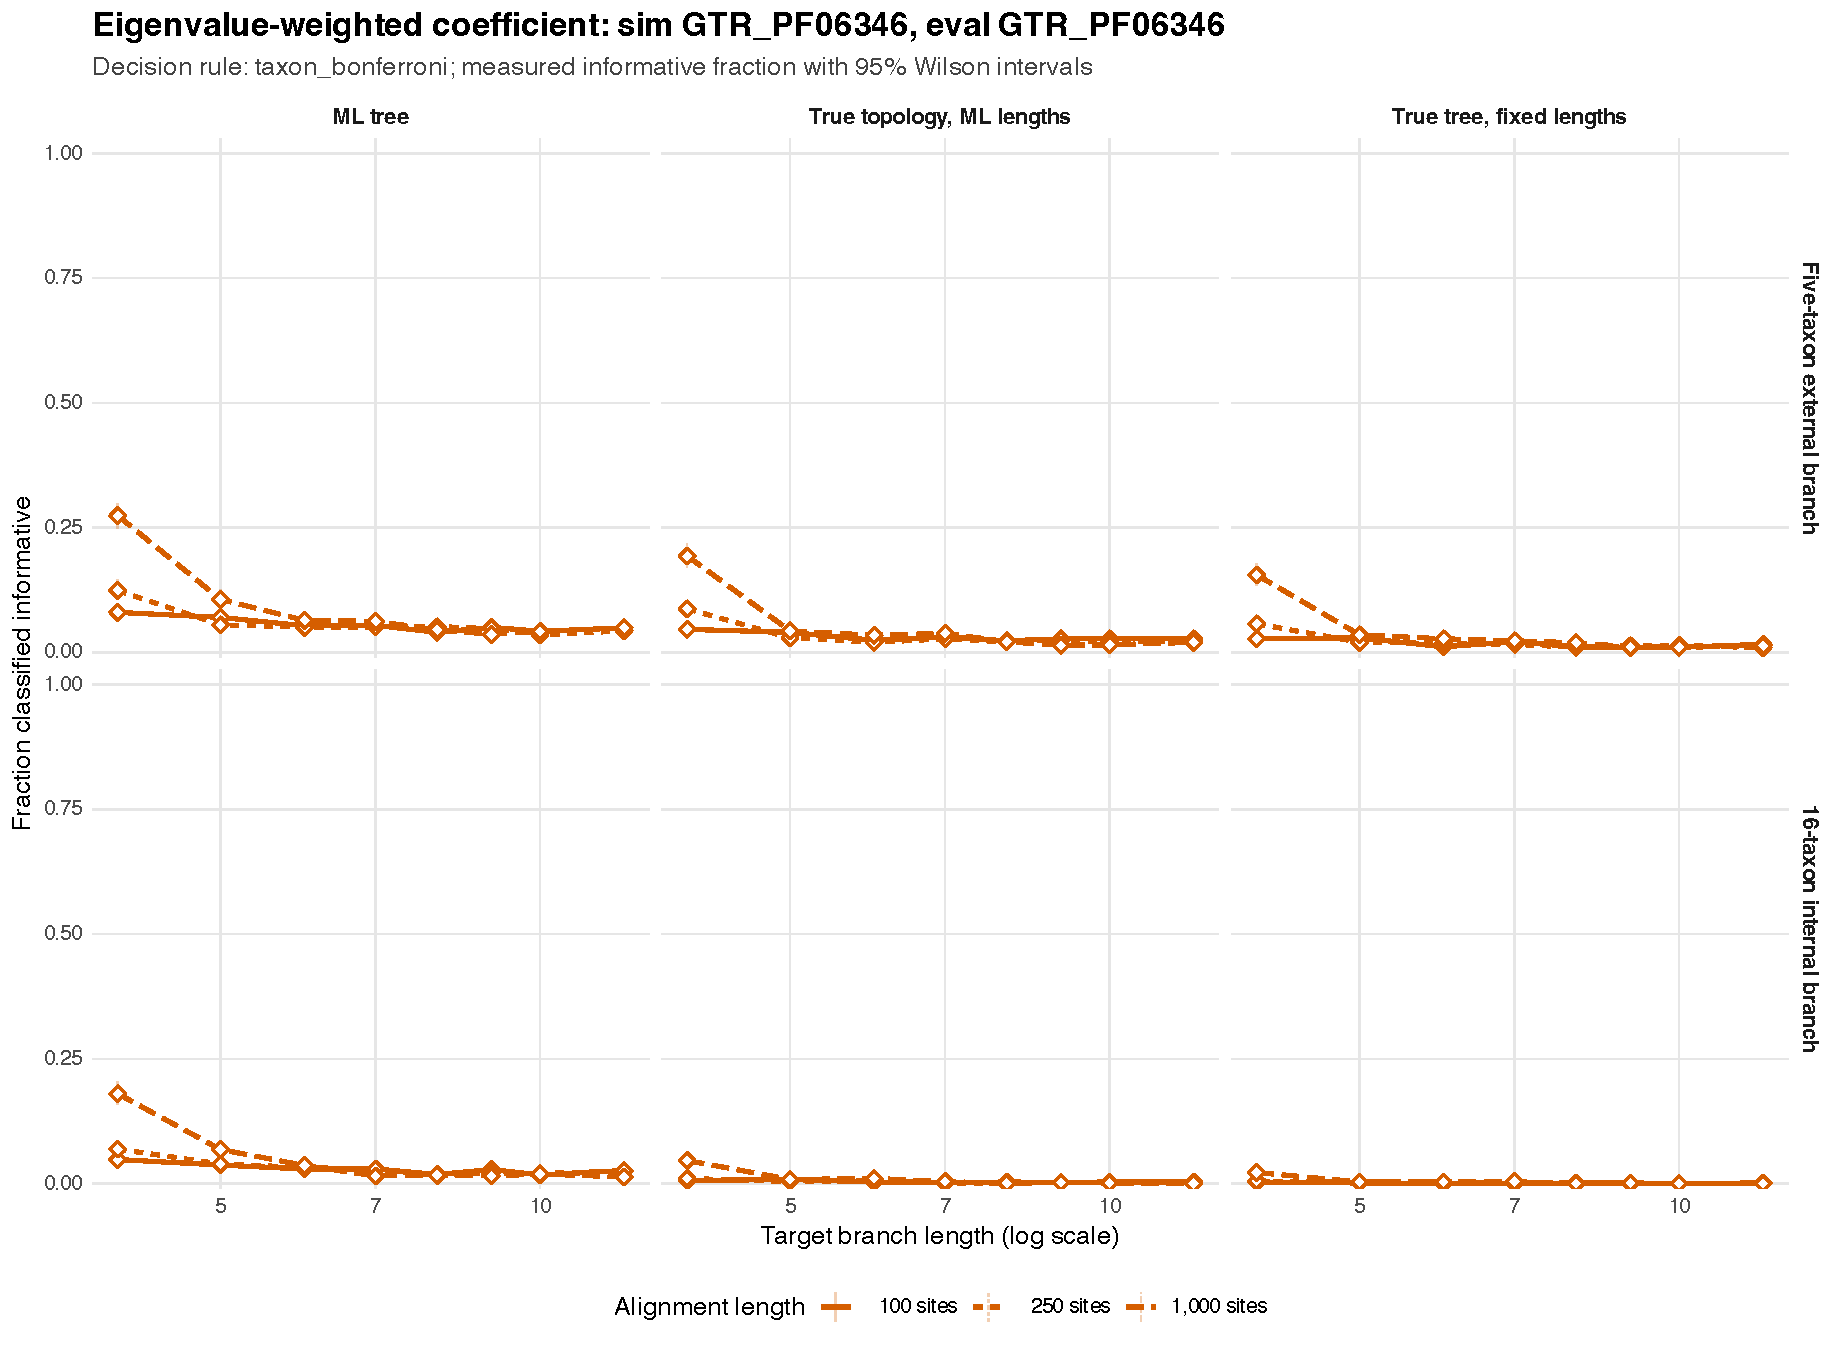
\includegraphics[width=0.49\textwidth]{figures/publication-suite/power/gtr_GTR_PF06346_weighted.pdf}
  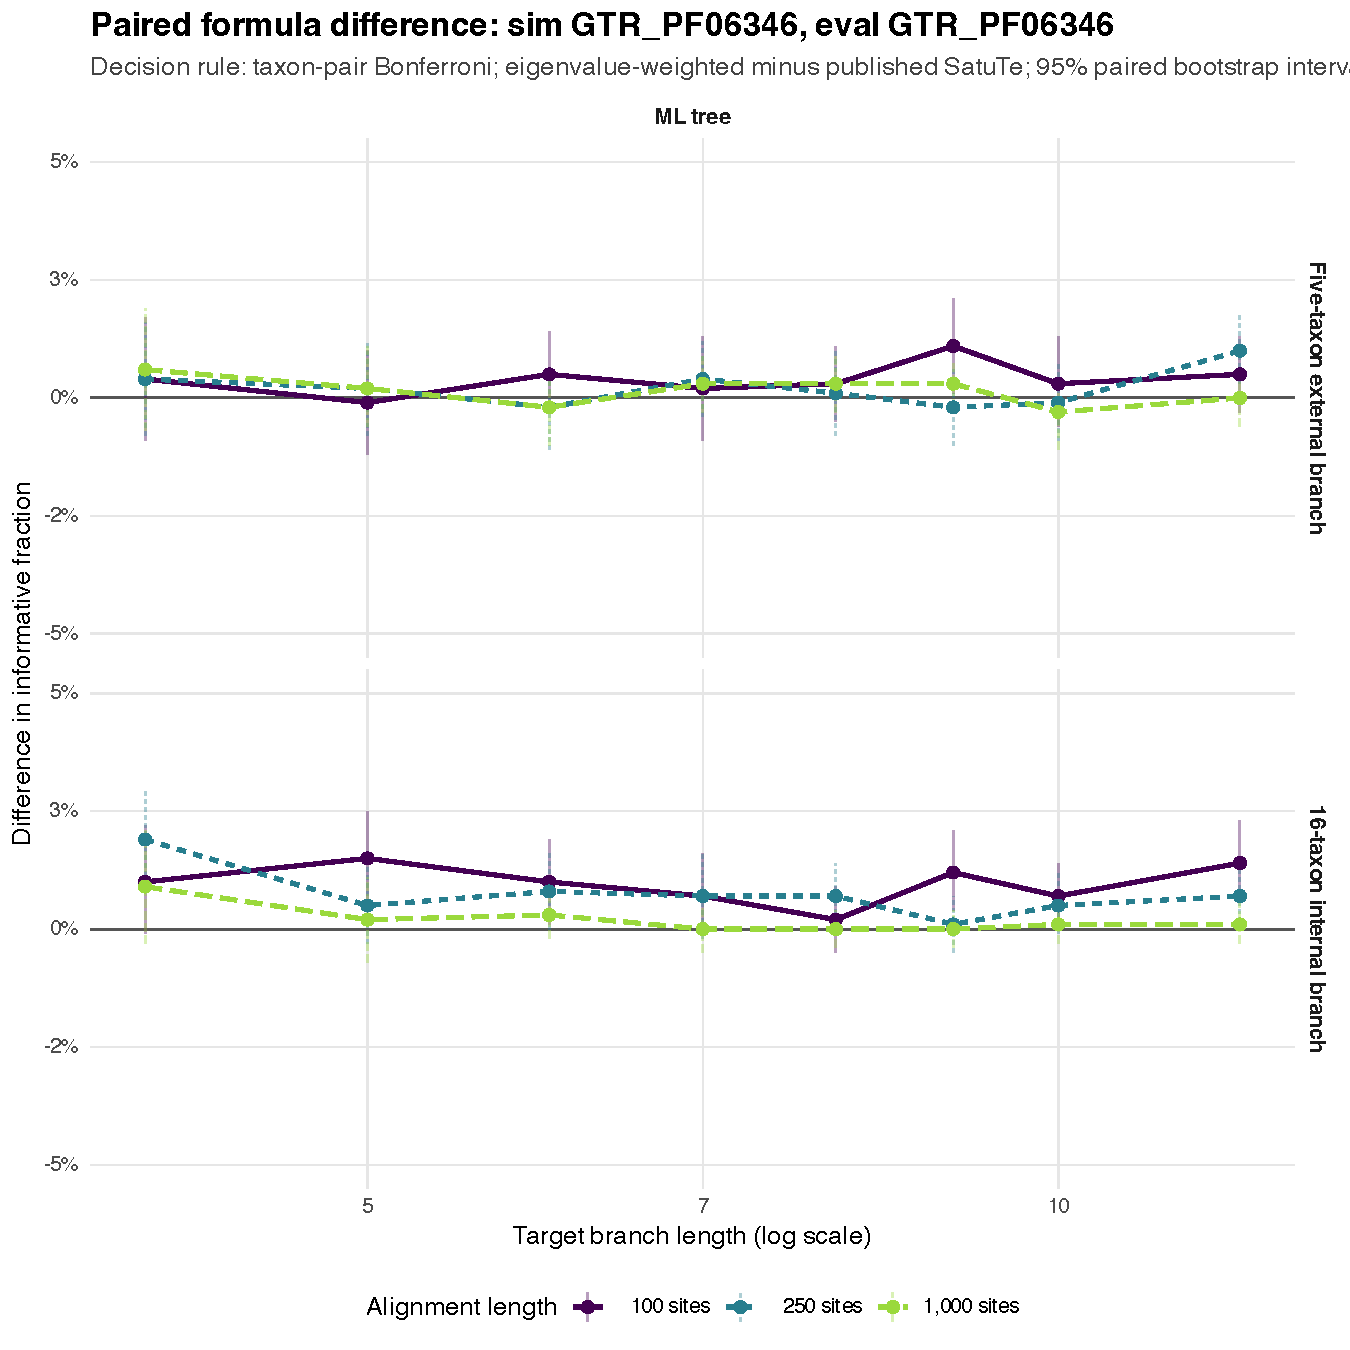
\includegraphics[width=0.72\textwidth]{figures/publication-suite/power/gtr_GTR_PF06346_difference.pdf}
  \caption{\textbf{Matched GTR+F power.} Dominant (top left), eigenvalue-weighted (top right) and paired difference (bottom) under taxon Bonferroni. Differences are small and mixed in this homogeneous-rate control.}
  \makeatletter\cref@old@label{fig-supp-gtr-power-a}\makeatother
\end{figure}

\begin{figure}[p]
  \centering
  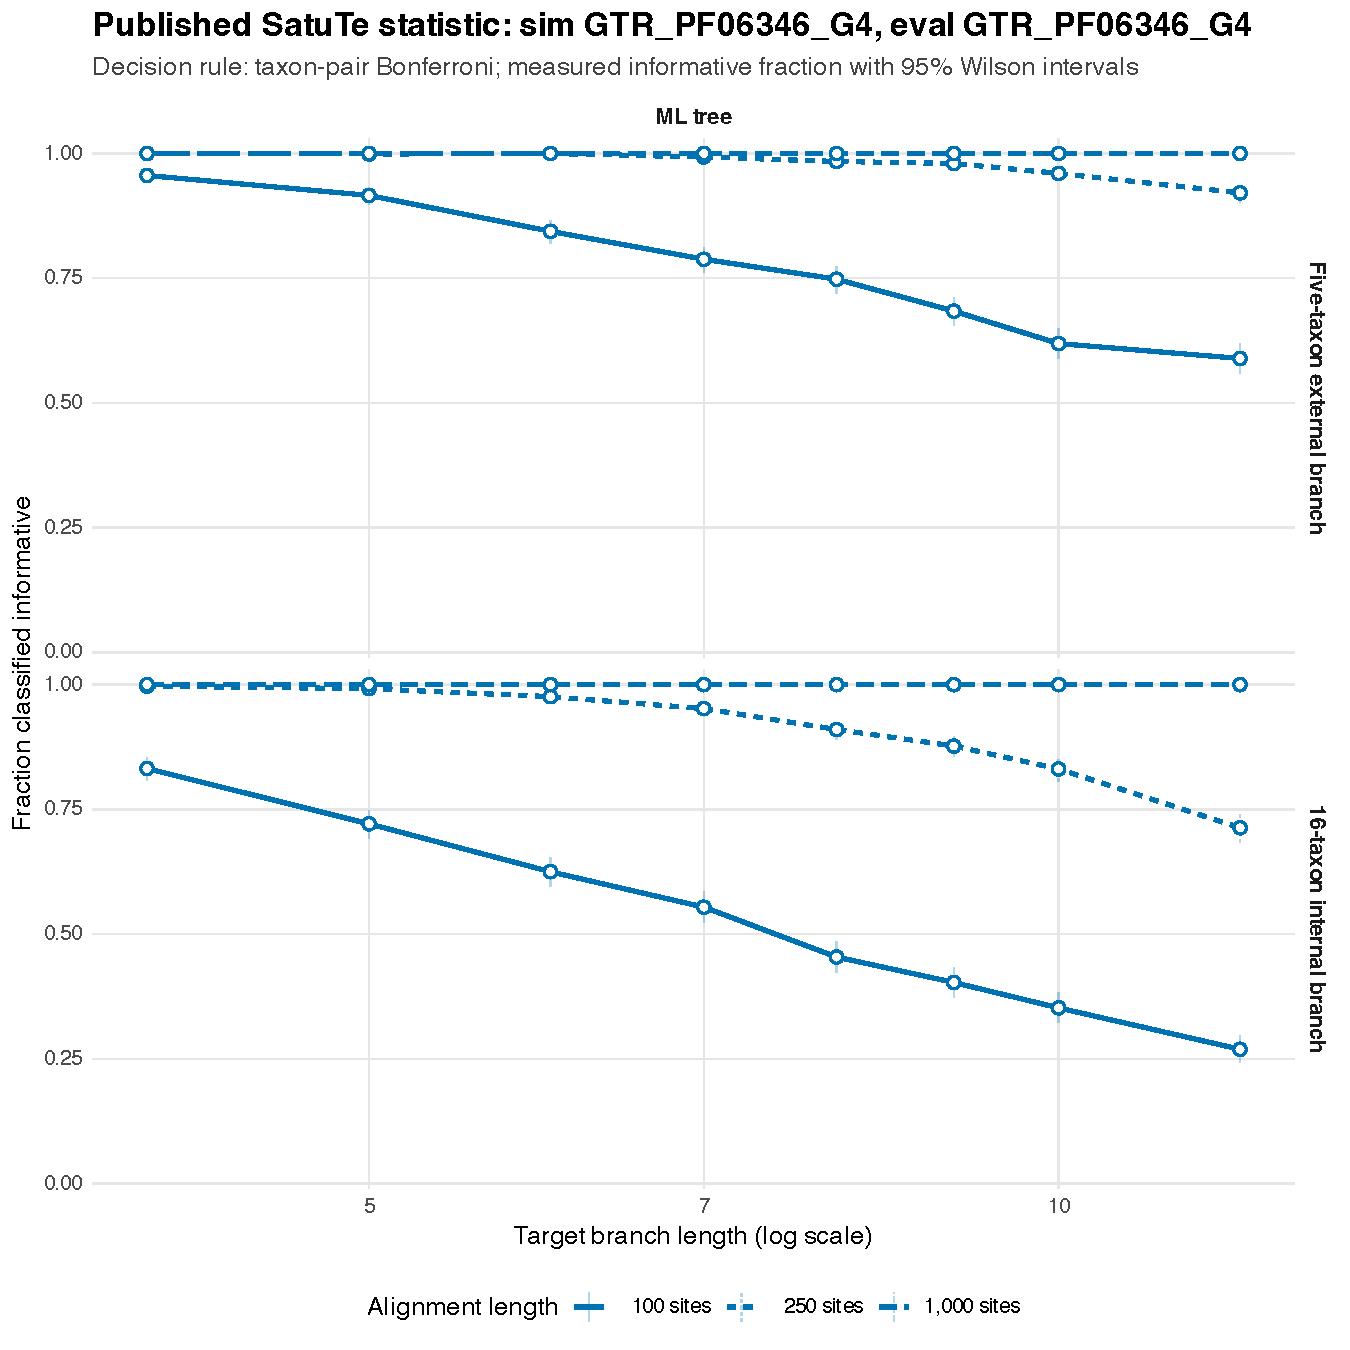
\includegraphics[width=0.49\textwidth]{figures/publication-suite/power/gtr_GTR_PF06346_G4_dominant.pdf}
  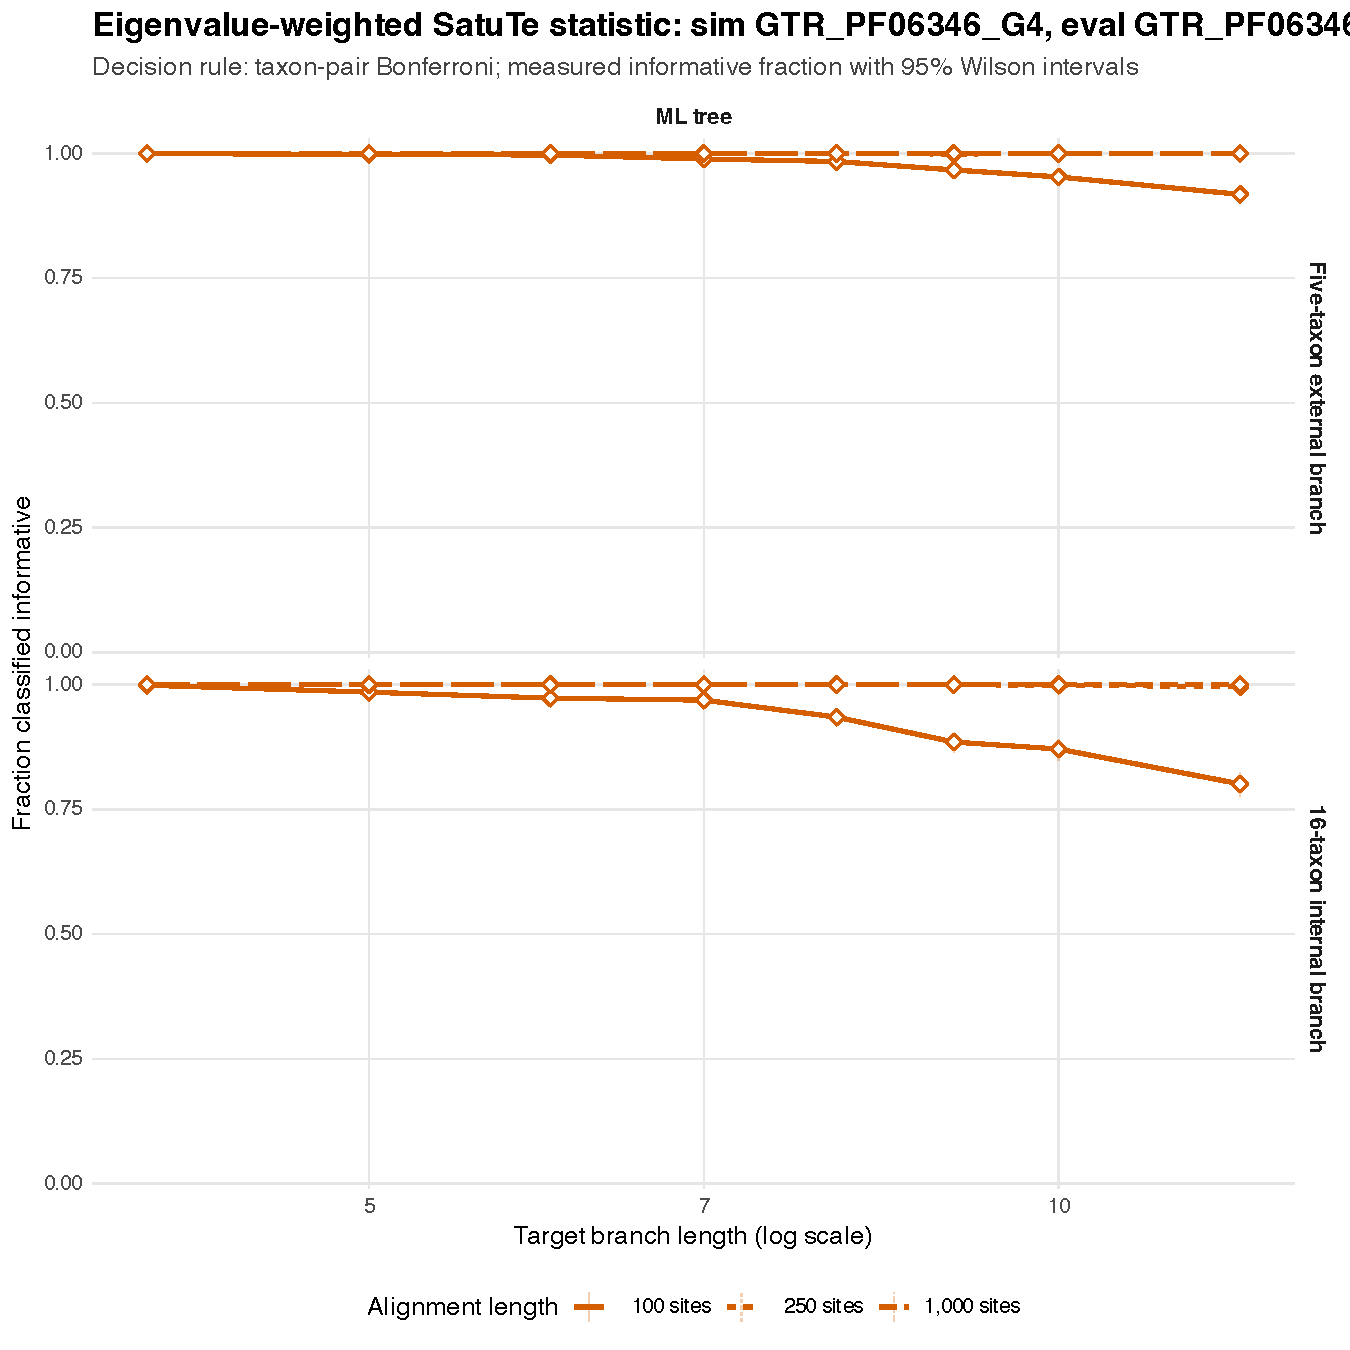
\includegraphics[width=0.49\textwidth]{figures/publication-suite/power/gtr_GTR_PF06346_G4_weighted.pdf}
  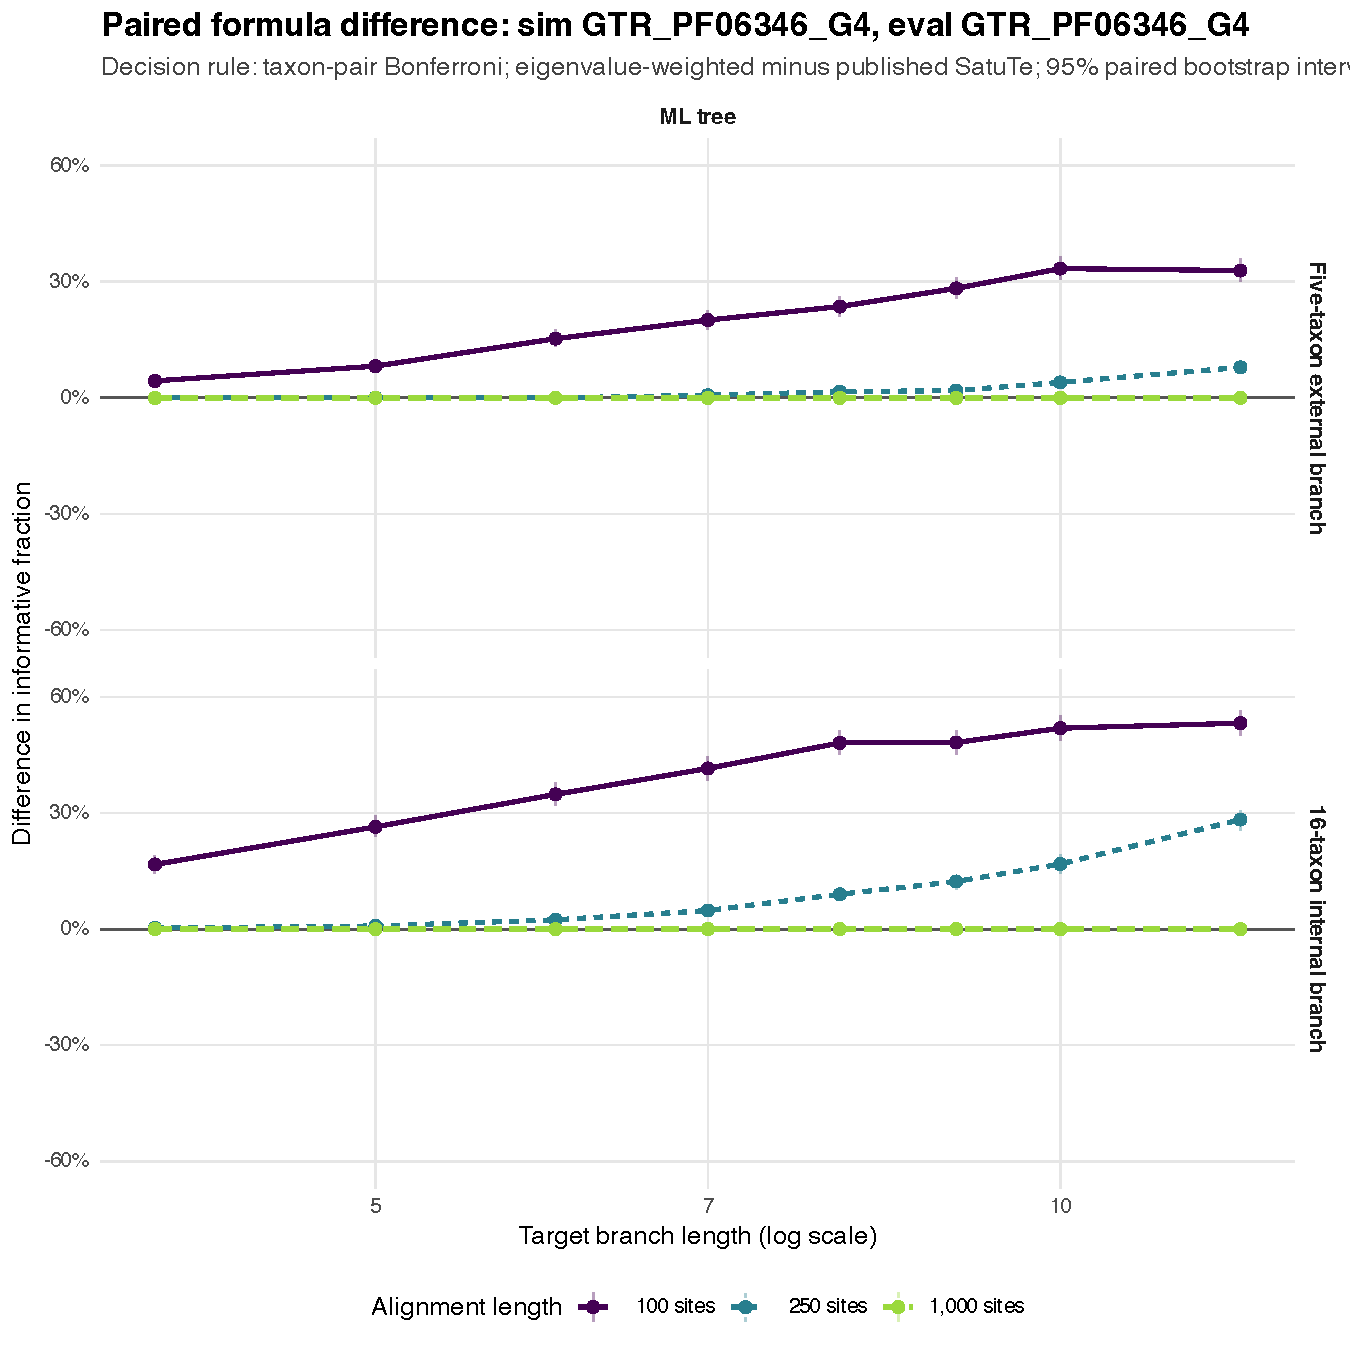
\includegraphics[width=0.72\textwidth]{figures/publication-suite/power/gtr_GTR_PF06346_G4_difference.pdf}
  \caption{\textbf{Matched GTR+F+G4 power.} Dominant (top left), eigenvalue-weighted (top right) and paired difference (bottom) under taxon Bonferroni. The weighted formula is never worse across the evaluated cells and yields gains of up to 57.6 percentage points.}
  \makeatletter\cref@old@label{fig-supp-gtr-power-b}\makeatother
\end{figure}

\begin{figure}[p]
  \centering
  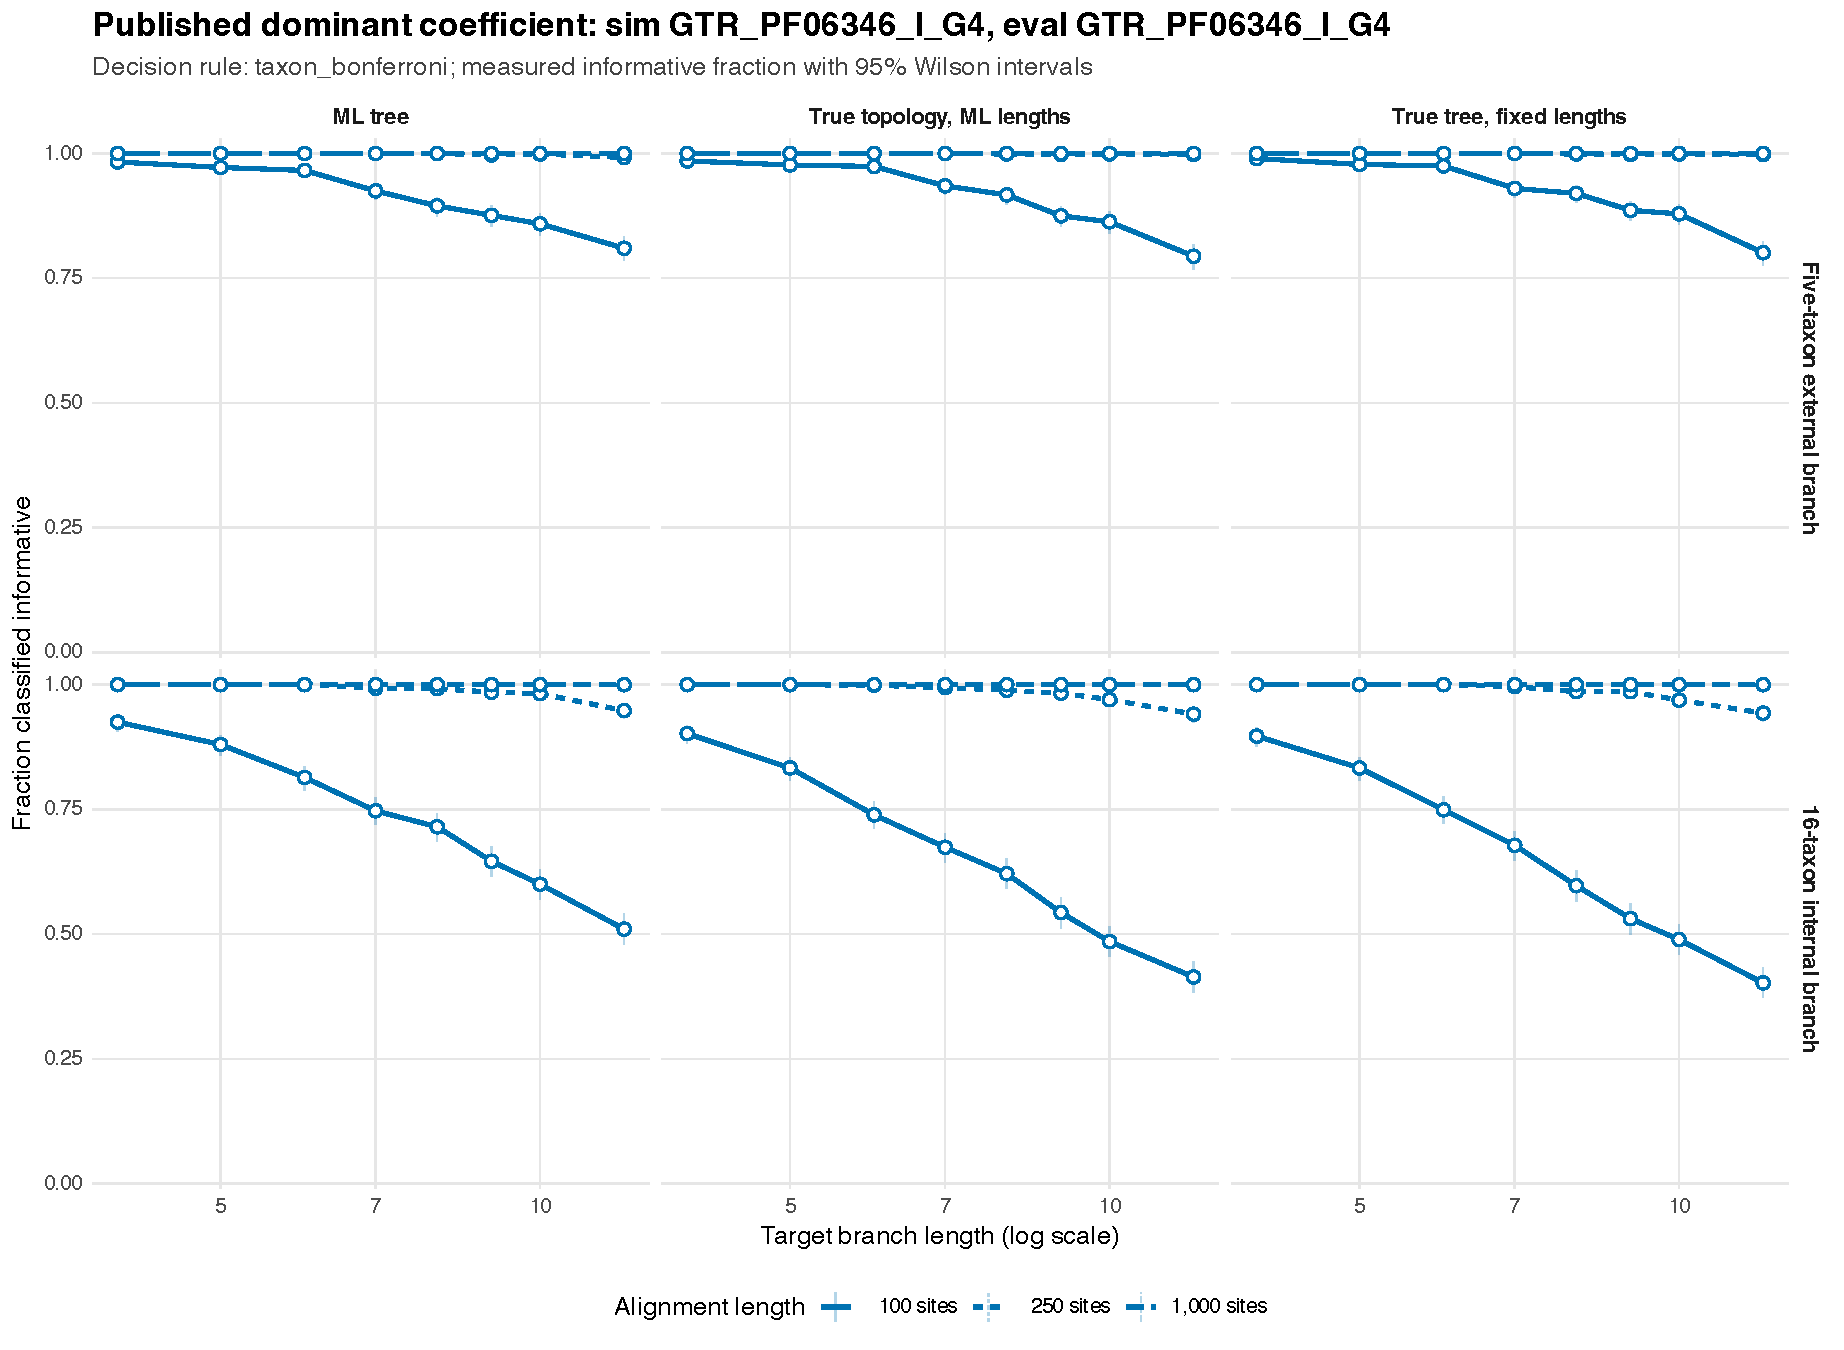
\includegraphics[width=0.49\textwidth]{figures/publication-suite/power/gtr_GTR_PF06346_I_G4_dominant.pdf}
  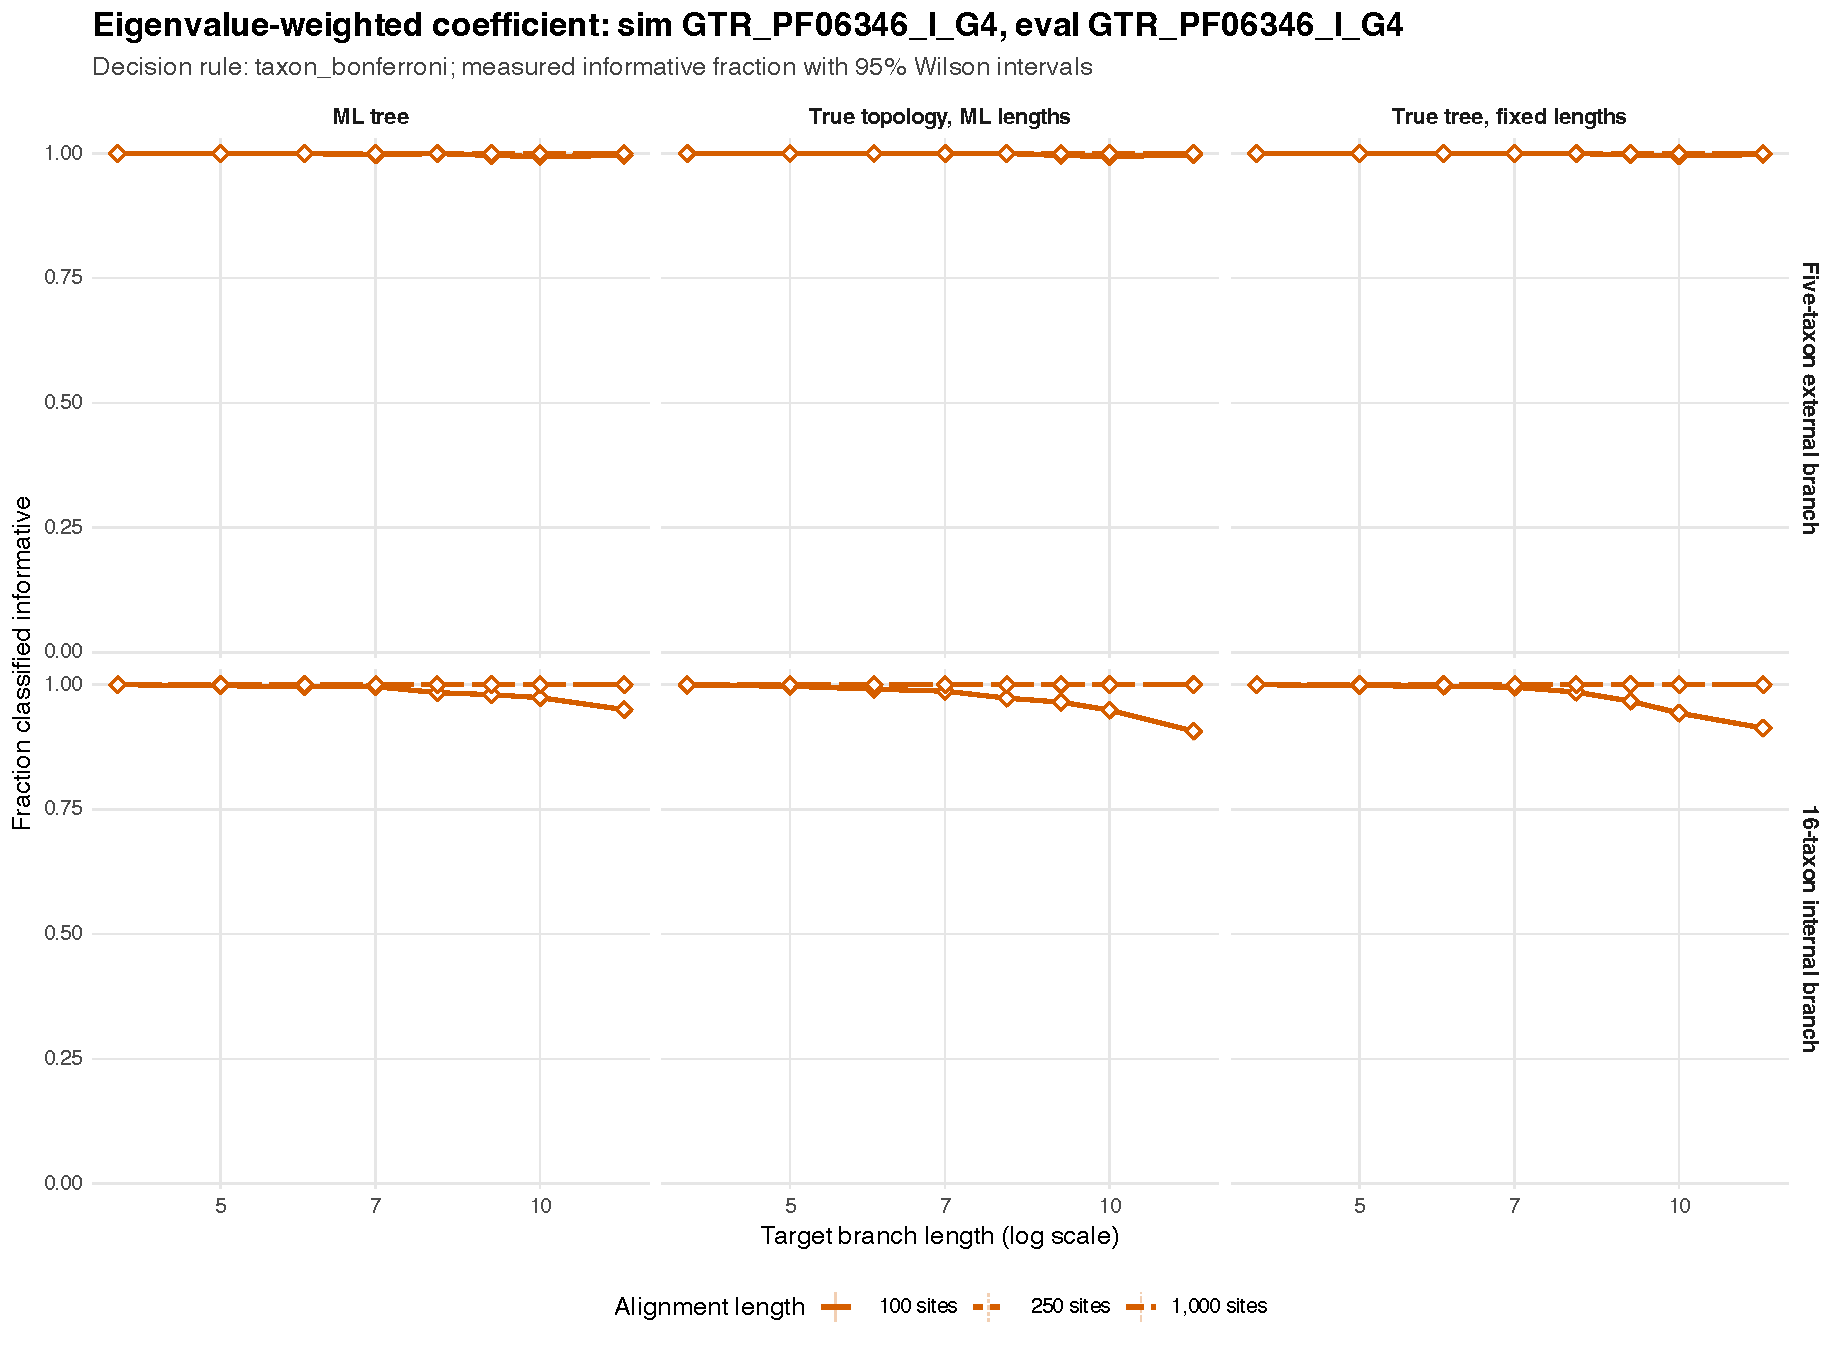
\includegraphics[width=0.49\textwidth]{figures/publication-suite/power/gtr_GTR_PF06346_I_G4_weighted.pdf}
  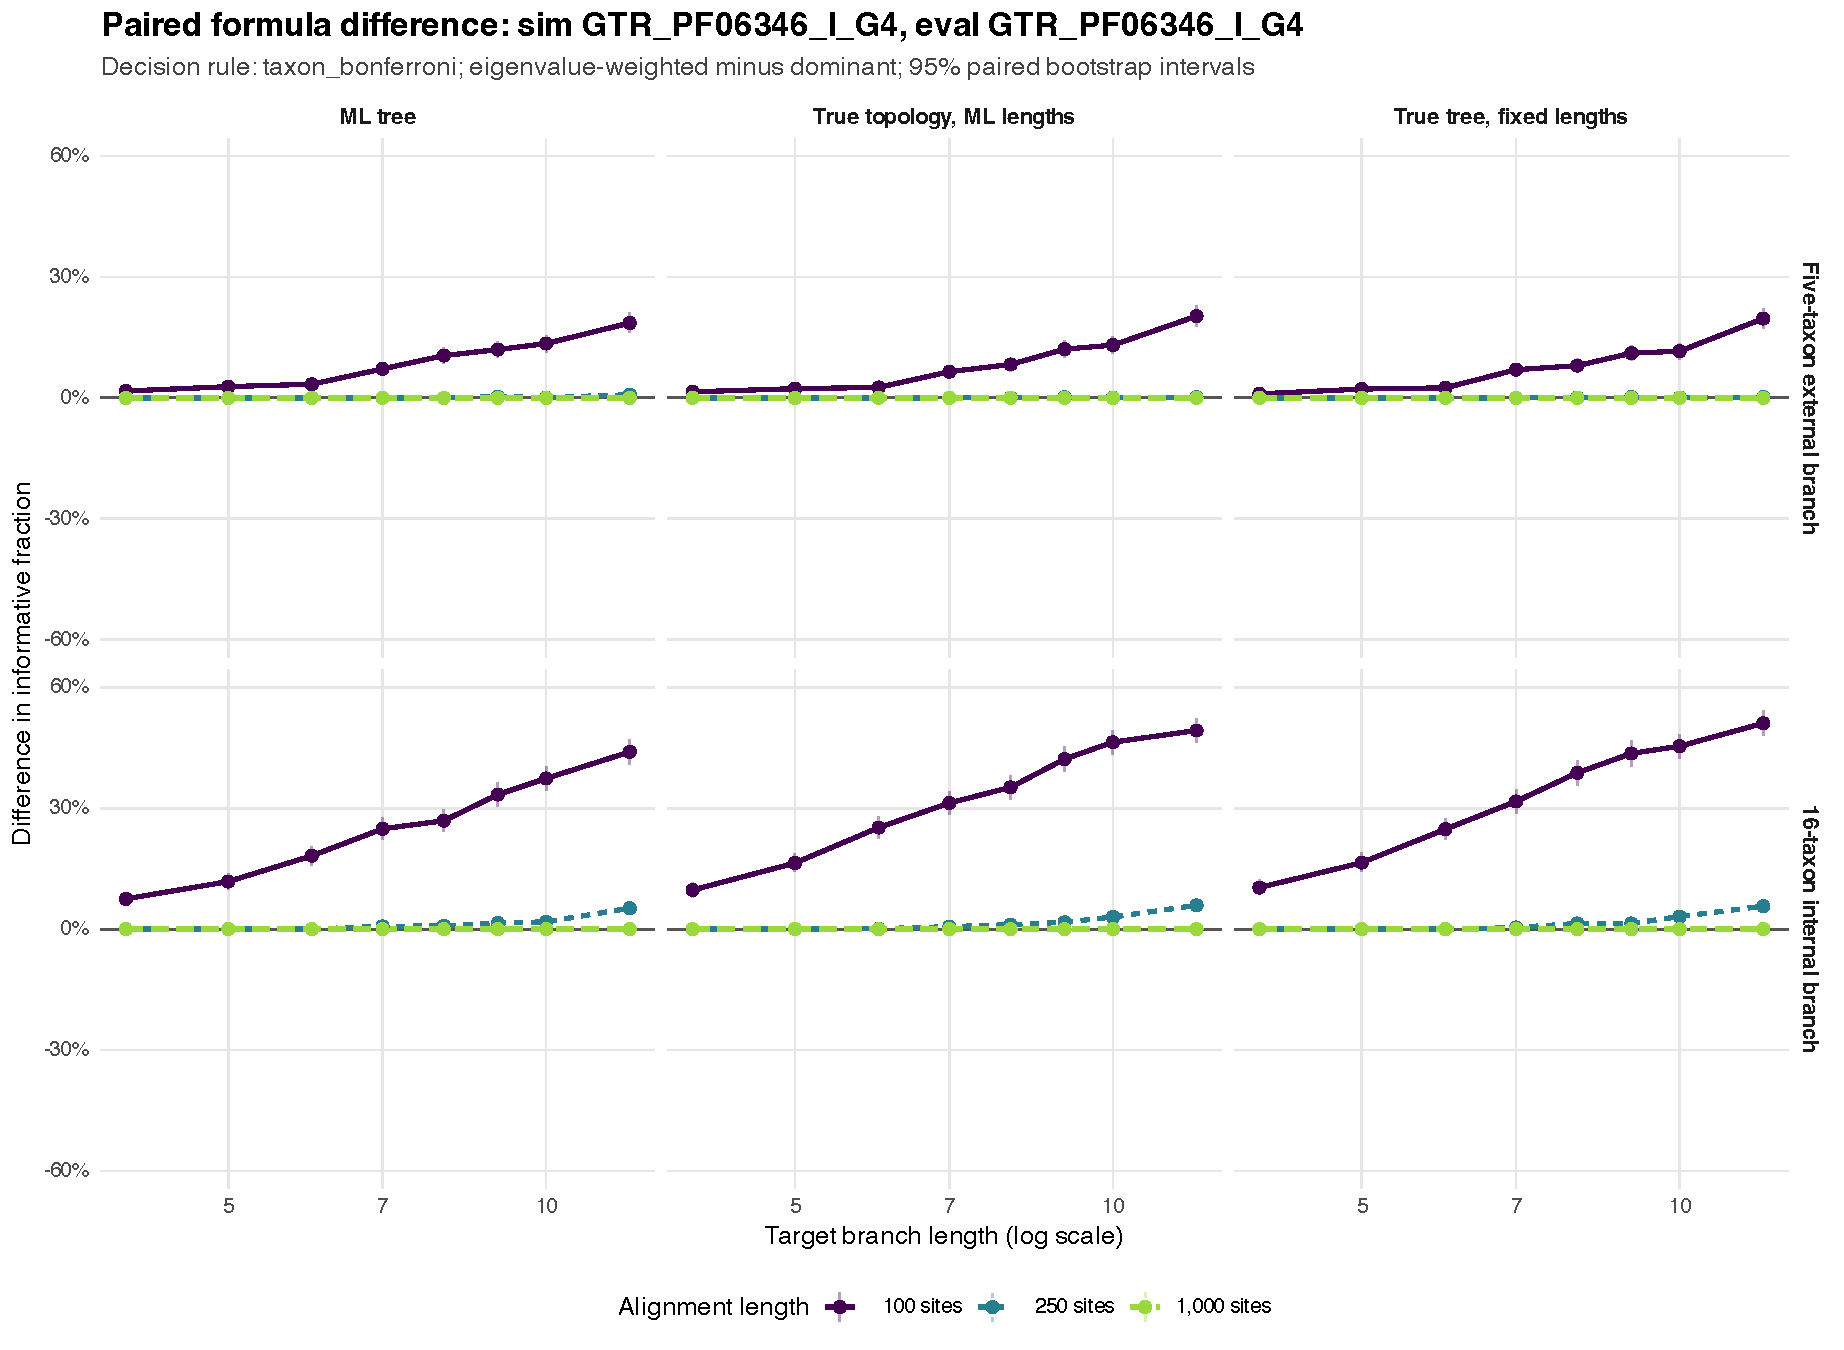
\includegraphics[width=0.72\textwidth]{figures/publication-suite/power/gtr_GTR_PF06346_I_G4_difference.pdf}
  \caption{\textbf{Matched GTR+F+I+G4 power.} Dominant (top left), eigenvalue-weighted (top right) and paired difference (bottom) under taxon Bonferroni. The invariant category is handled by the corrected mixture null; weighting is never worse across the evaluated cells and gains up to 51.1 percentage points.}
  \makeatletter\cref@old@label{fig-supp-gtr-power-c}\makeatother
\end{figure}

\begin{figure}[p]
  \centering
  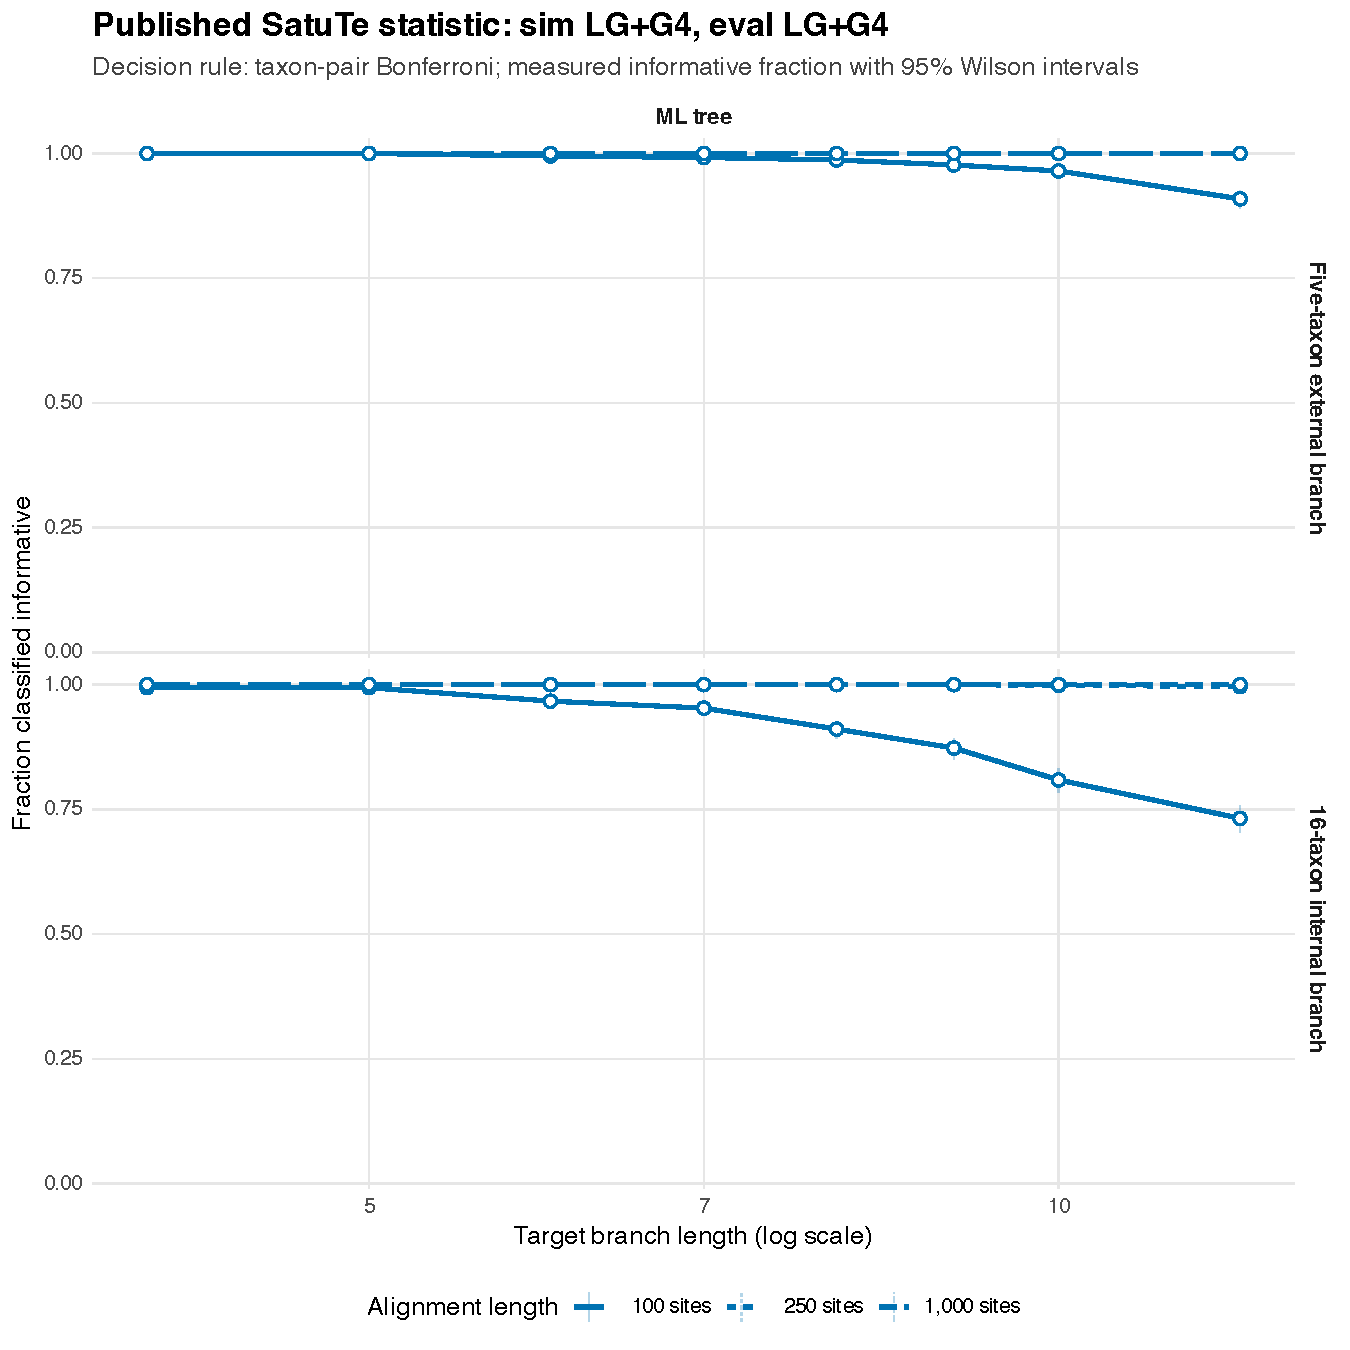
\includegraphics[width=0.49\textwidth]{figures/publication-suite/power/protein_LG_G4_dominant.pdf}
  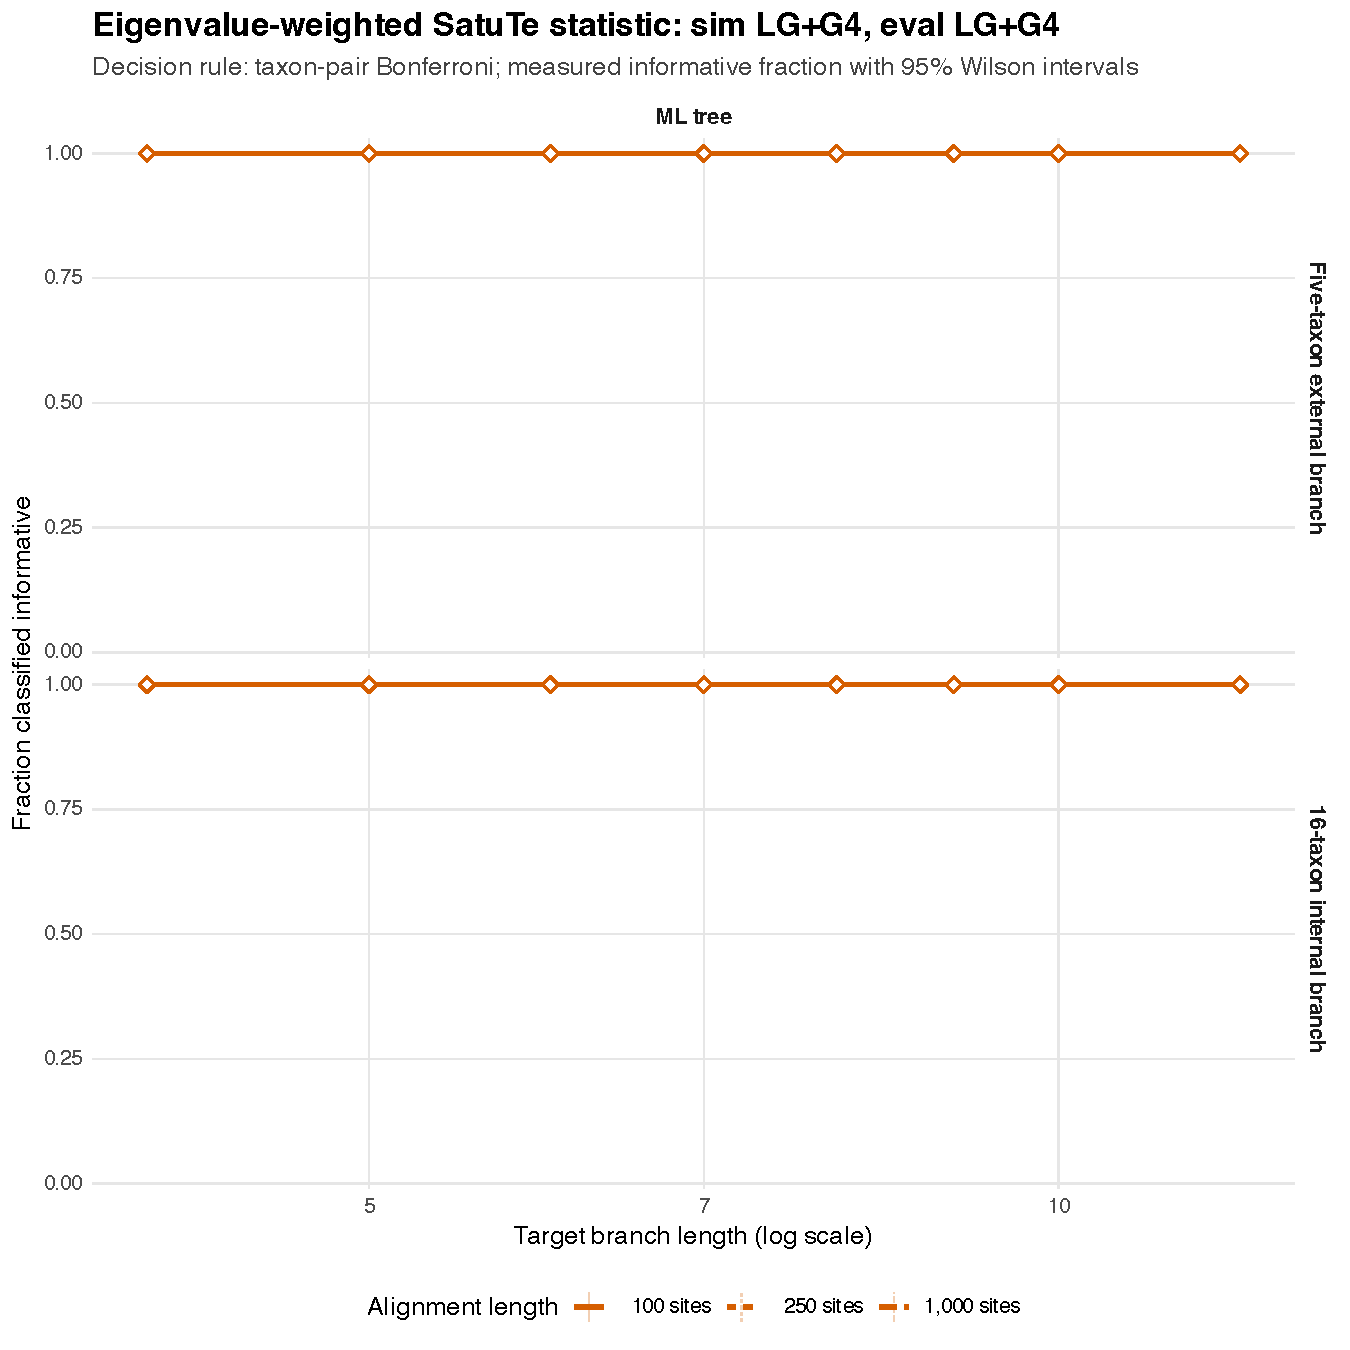
\includegraphics[width=0.49\textwidth]{figures/publication-suite/power/protein_LG_G4_weighted.pdf}
  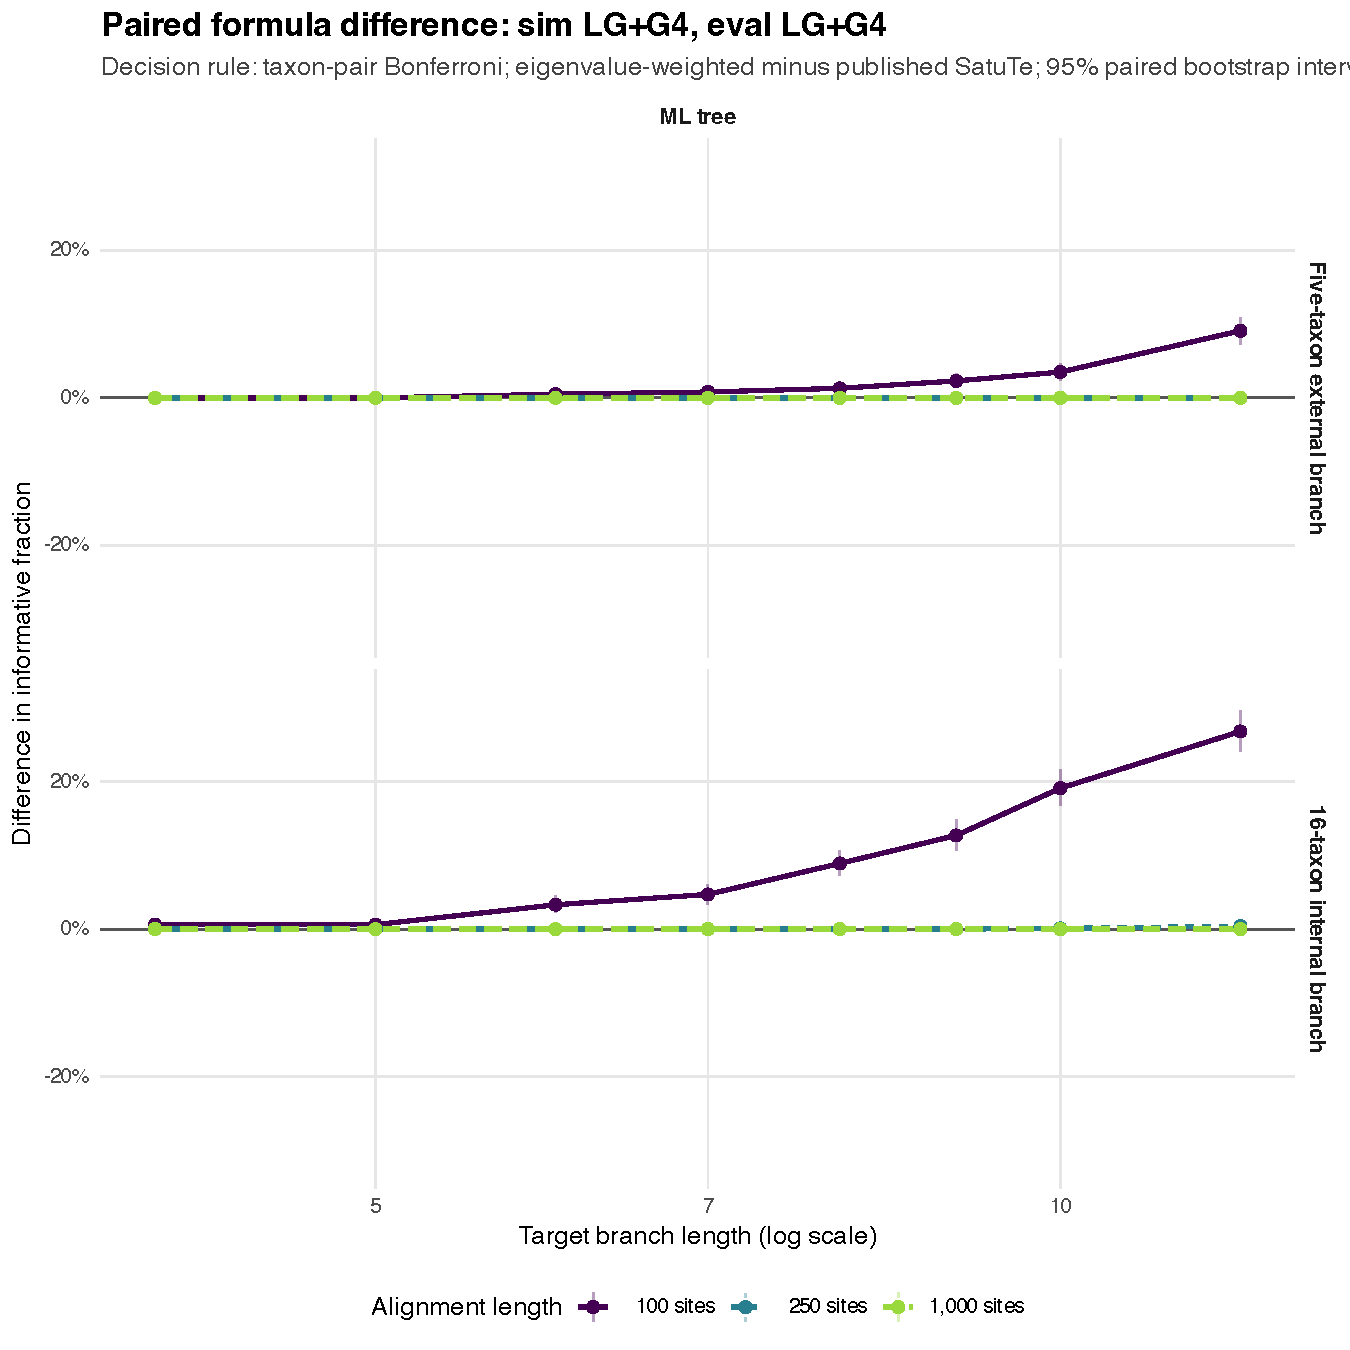
\includegraphics[width=0.72\textwidth]{figures/publication-suite/power/protein_LG_G4_difference.pdf}
  \caption{\textbf{Matched LG+G4 power.} Dominant (top left), weighted (top right) and weighted-minus-dominant difference (bottom) under taxon Bonferroni. Weighting is never worse across the evaluated cells and gains up to 32.7 percentage points.}
  \makeatletter\cref@old@label{fig-supp-protein-lg}\makeatother
\end{figure}

\begin{figure}[p]
  \centering
  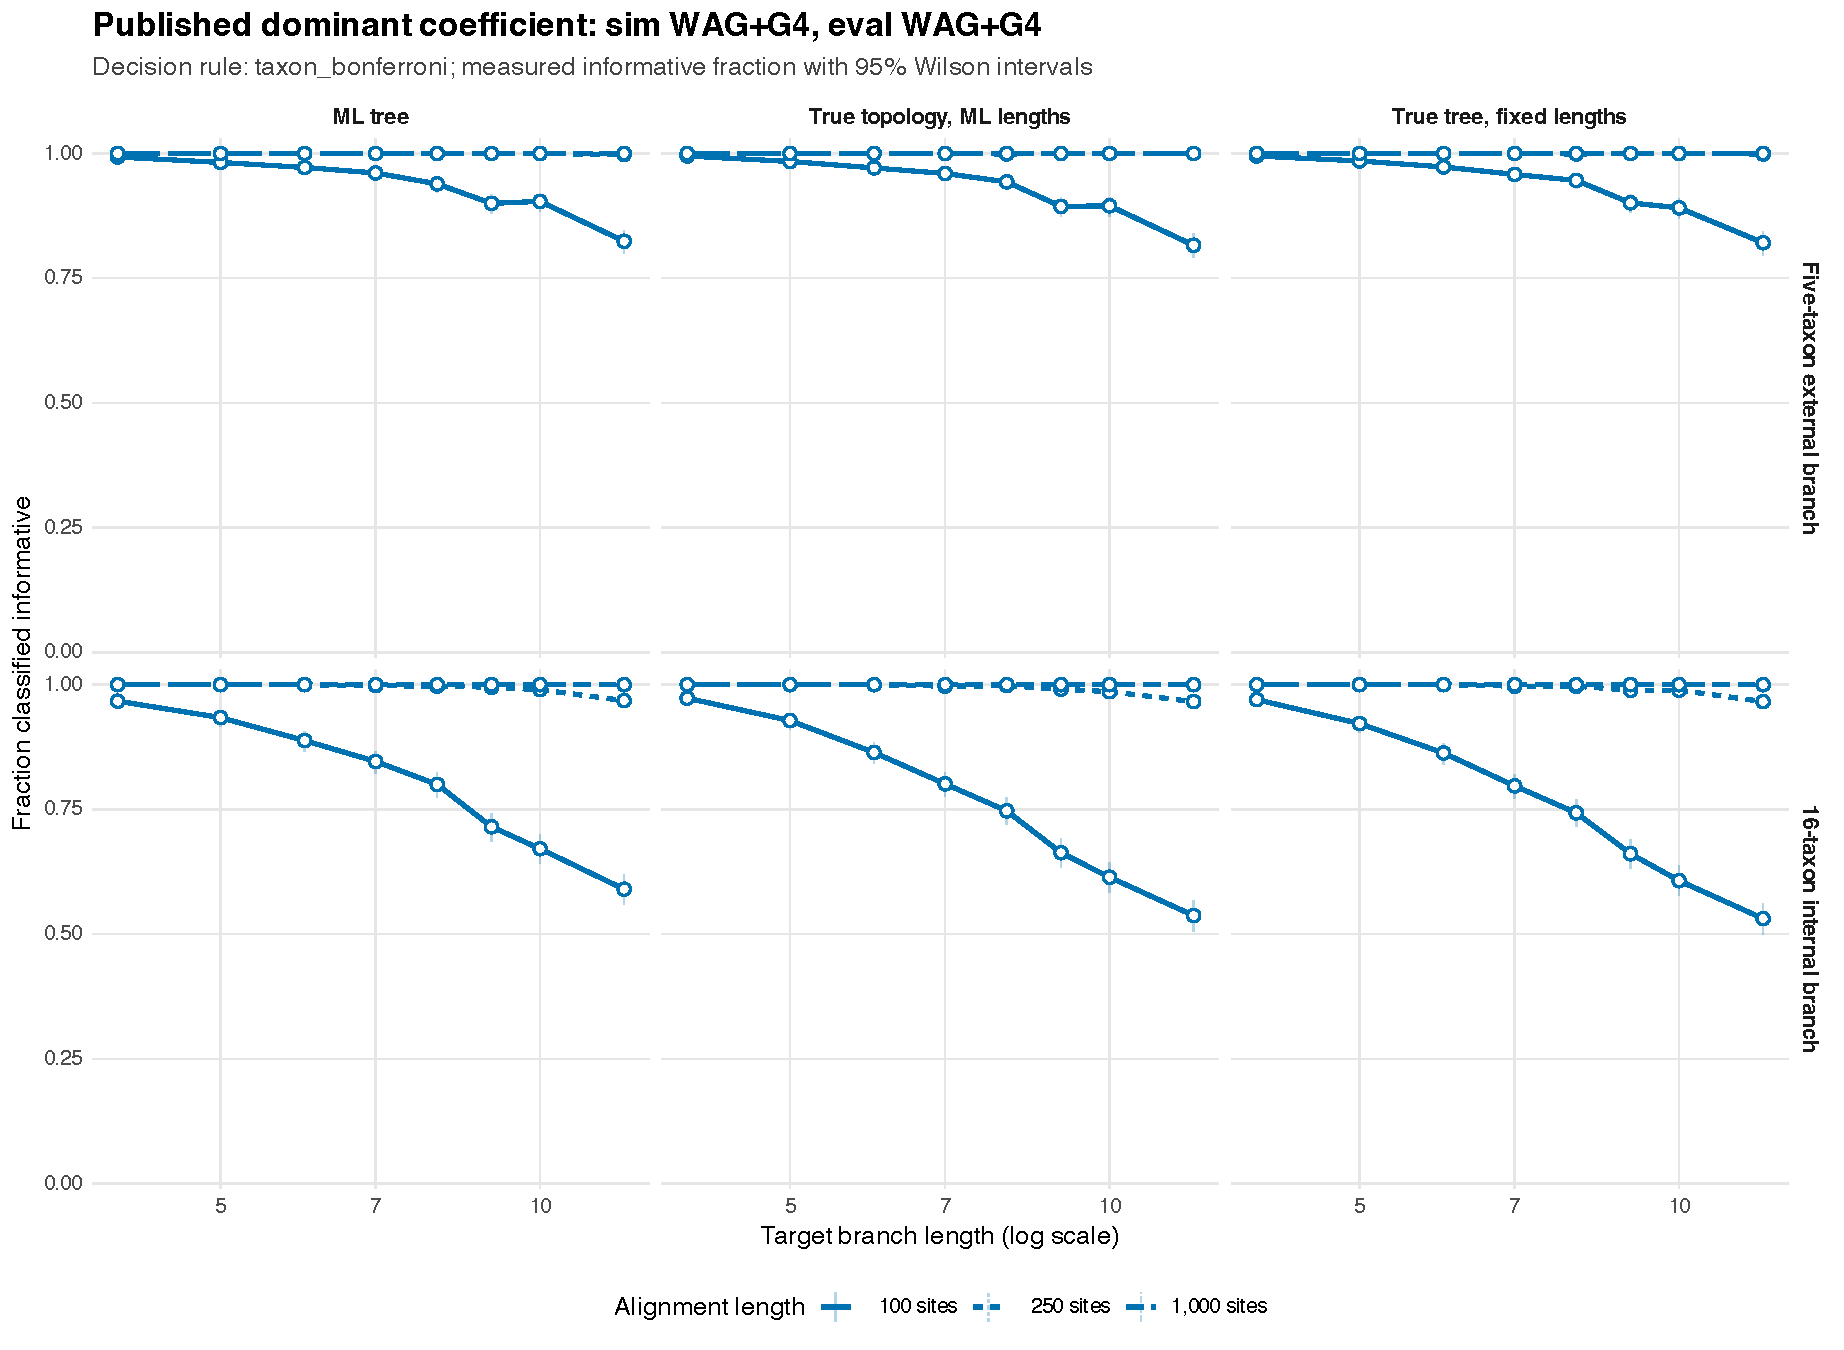
\includegraphics[width=0.49\textwidth]{figures/publication-suite/power/protein_WAG_G4_dominant.pdf}
  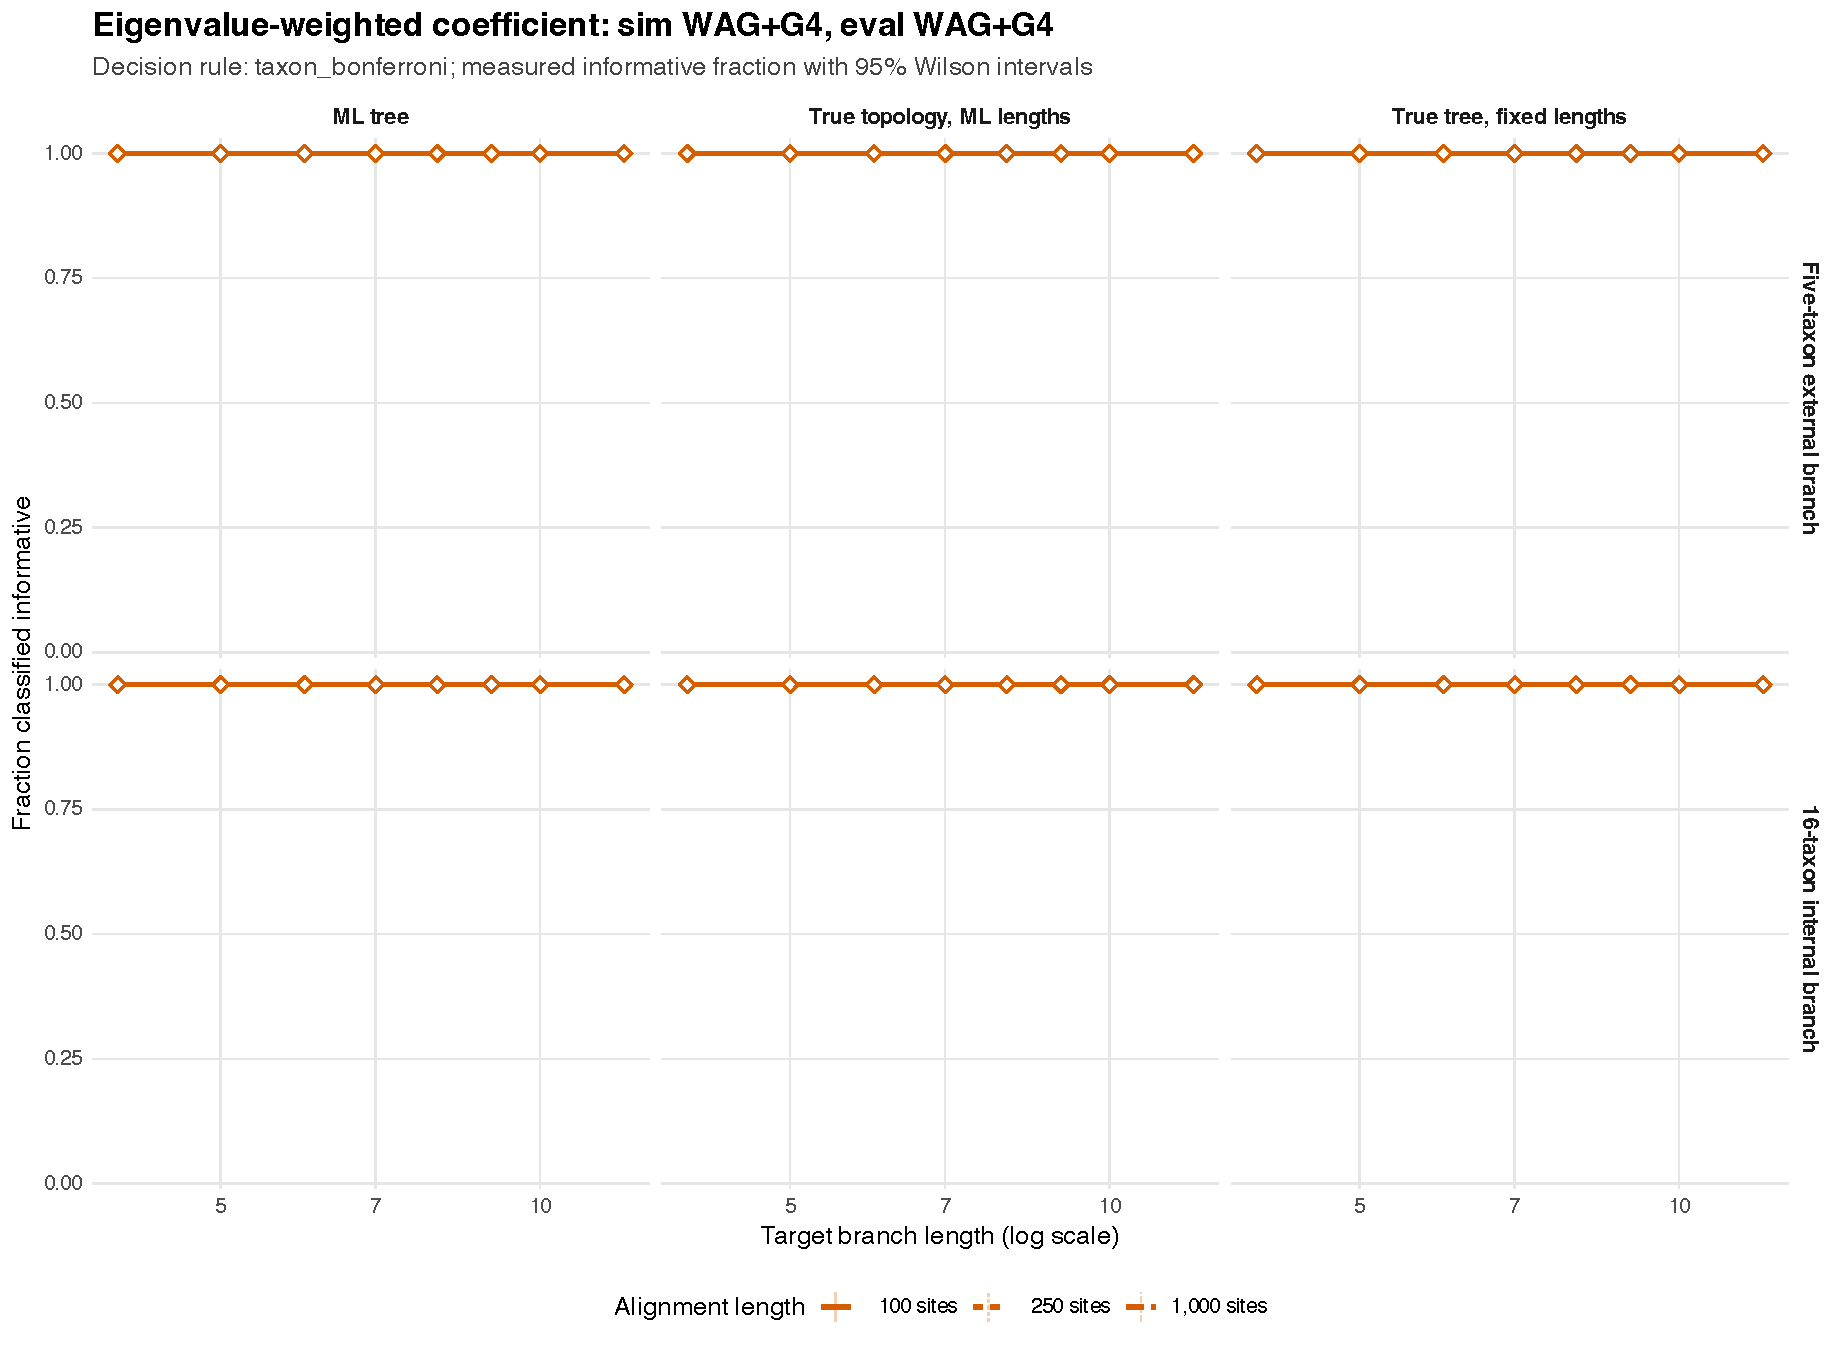
\includegraphics[width=0.49\textwidth]{figures/publication-suite/power/protein_WAG_G4_weighted.pdf}
  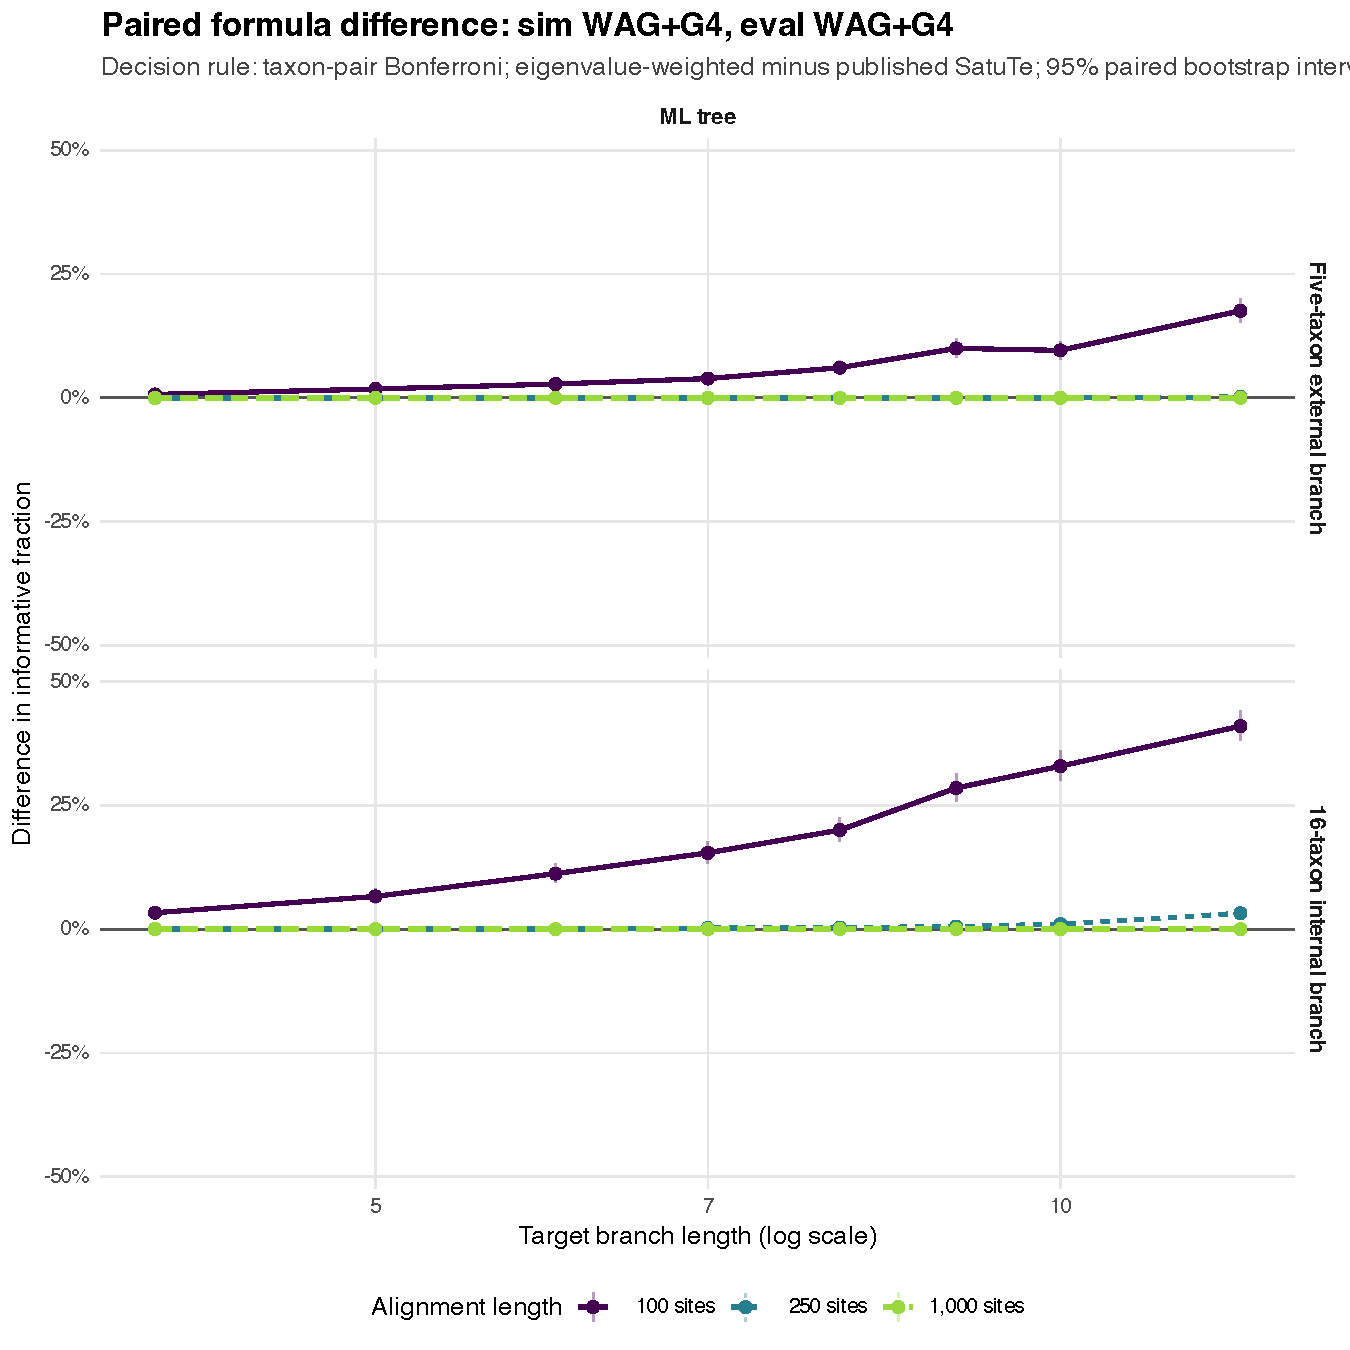
\includegraphics[width=0.72\textwidth]{figures/publication-suite/power/protein_WAG_G4_difference.pdf}
  \caption{\textbf{Matched WAG+G4 power.} Dominant (top left), weighted (top right) and weighted-minus-dominant difference (bottom) under taxon Bonferroni. Weighting is never worse across the evaluated cells and gains up to 46.9 percentage points.}
  \makeatletter\cref@old@label{fig-supp-protein-wag}\makeatother
\end{figure}

\begin{figure}[p]
  \centering
  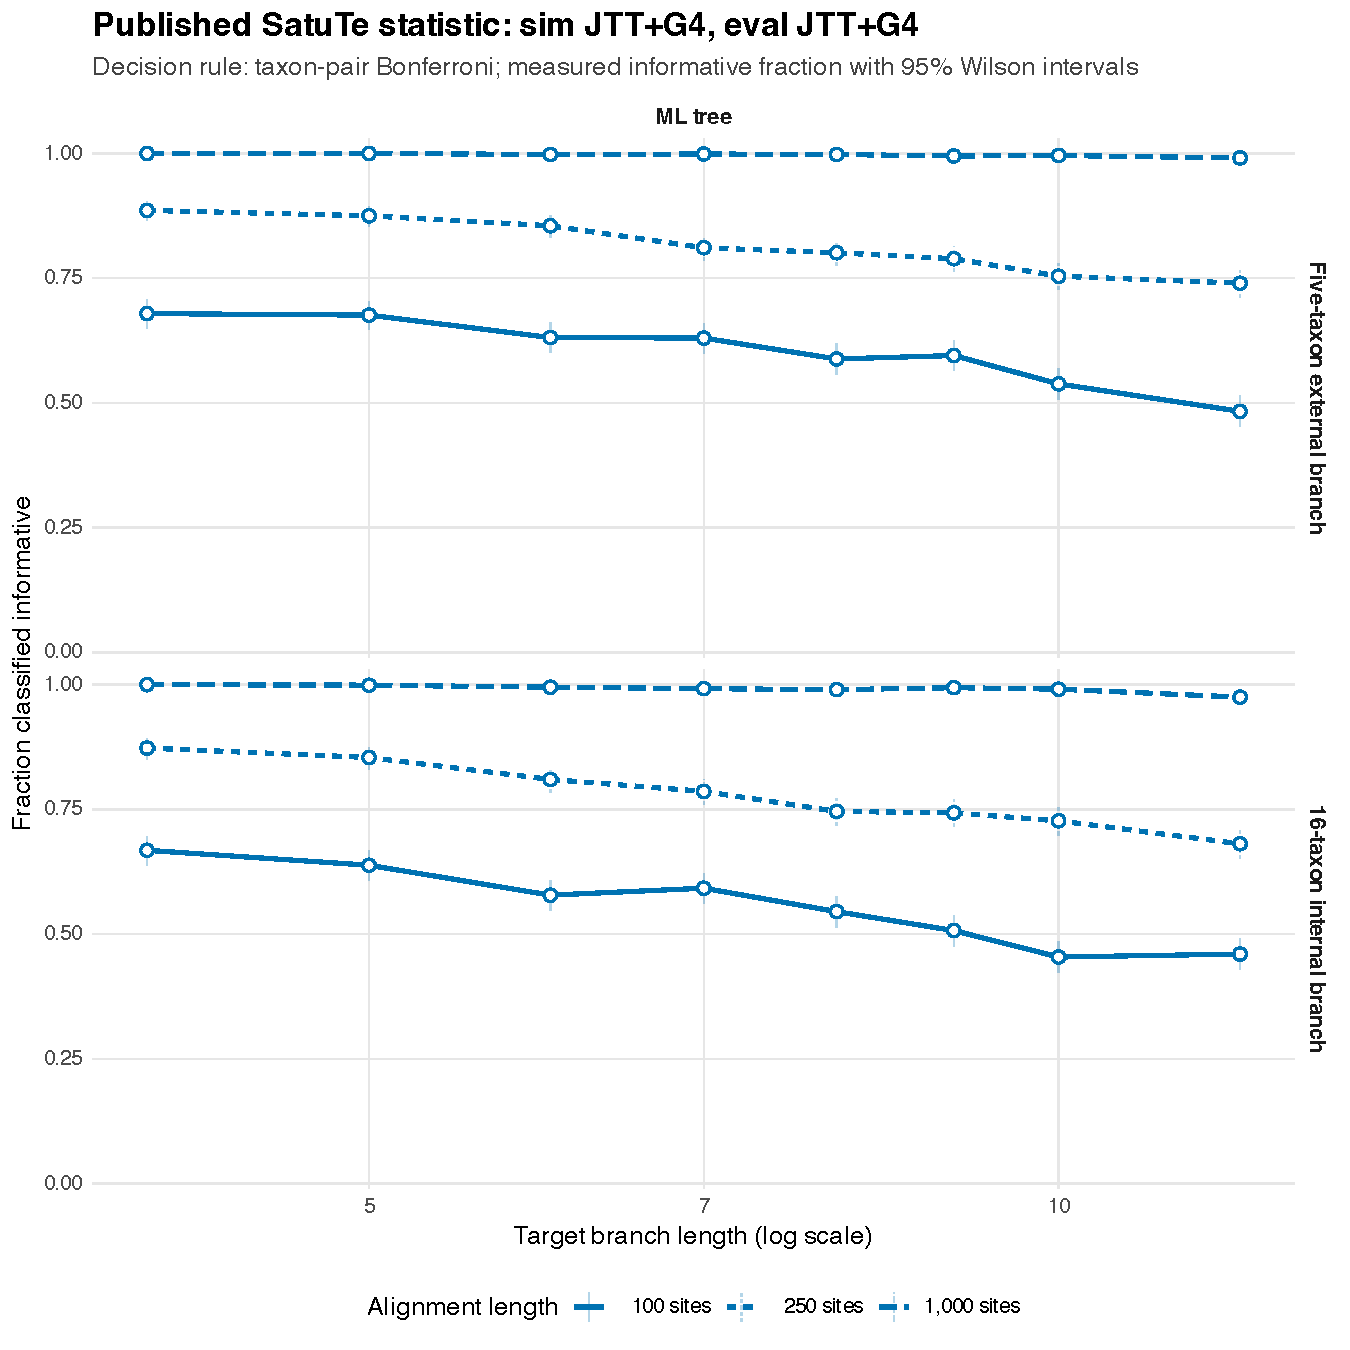
\includegraphics[width=0.49\textwidth]{figures/publication-suite/power/protein_JTT_G4_dominant.pdf}
  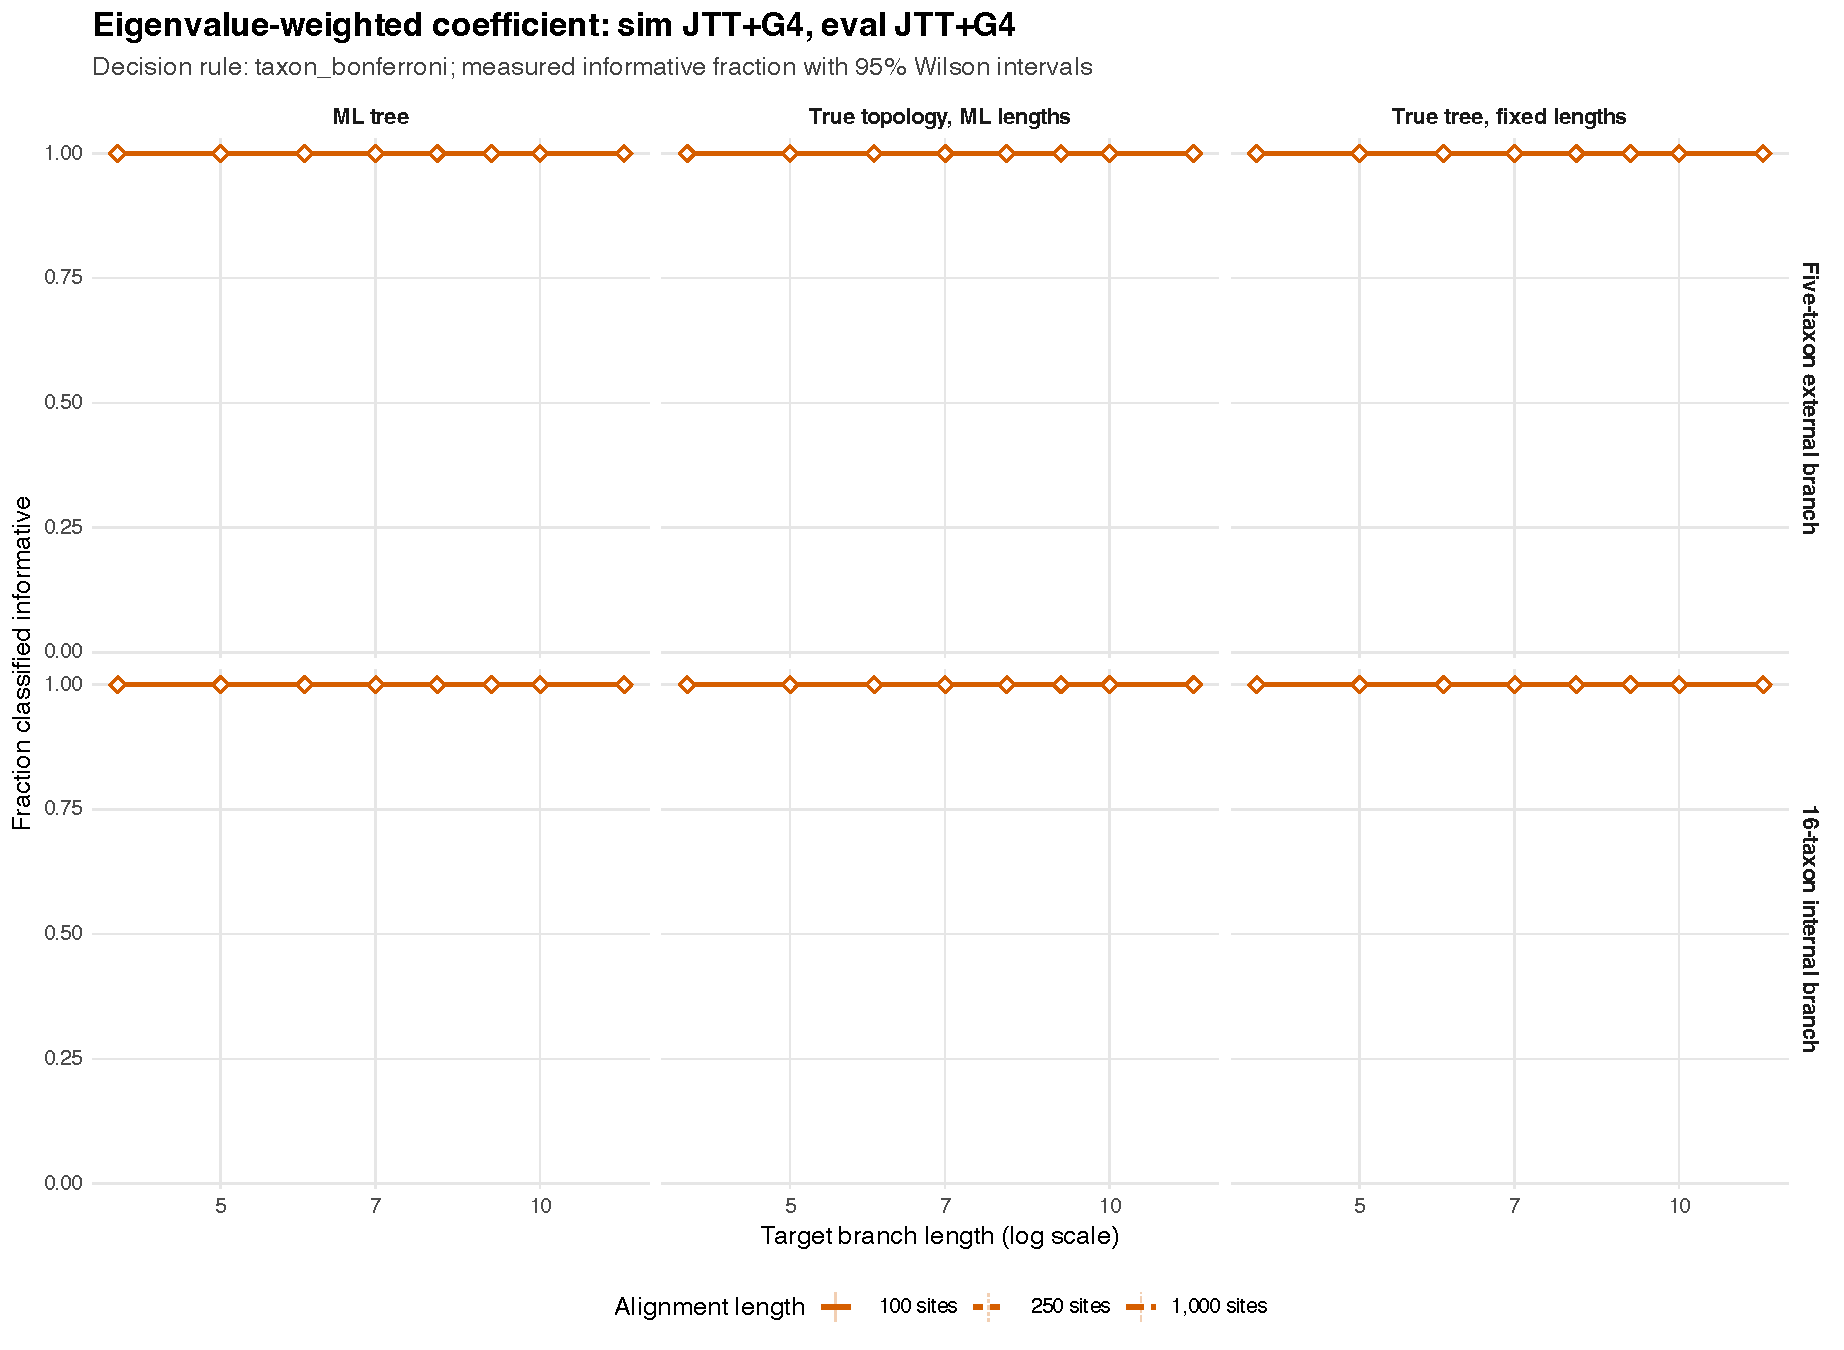
\includegraphics[width=0.49\textwidth]{figures/publication-suite/power/protein_JTT_G4_weighted.pdf}
  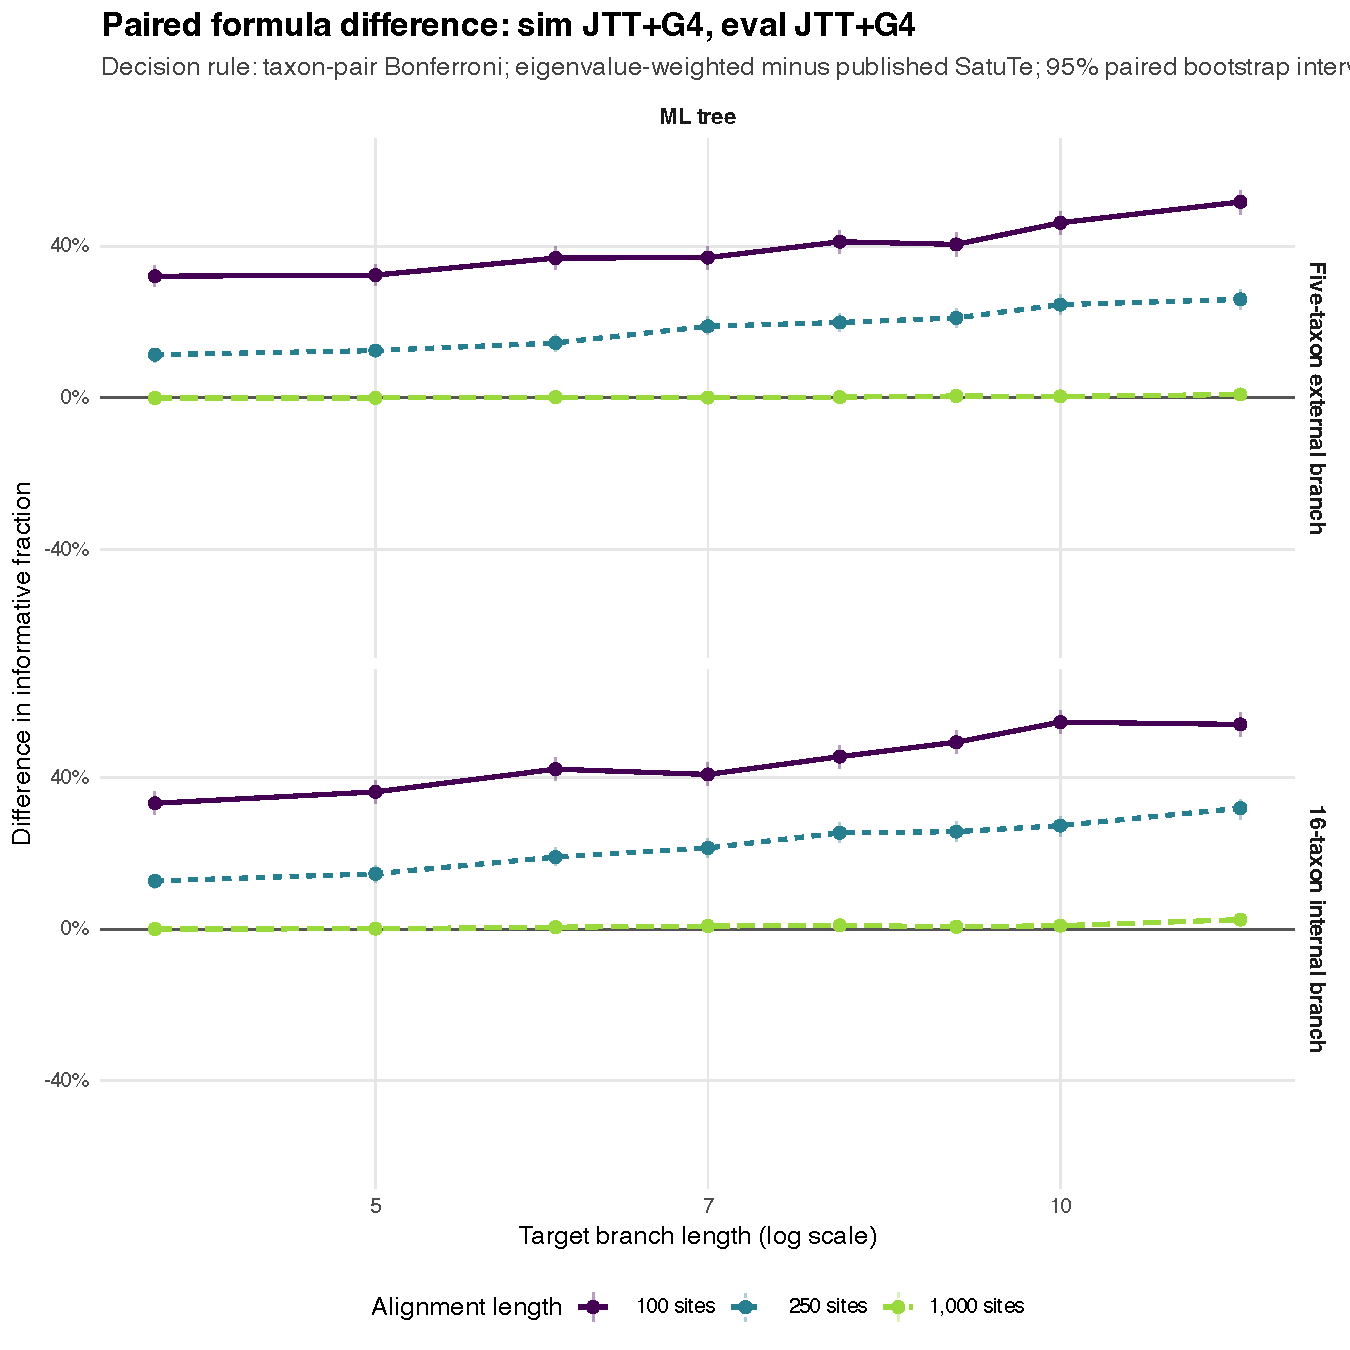
\includegraphics[width=0.72\textwidth]{figures/publication-suite/power/protein_JTT_G4_difference.pdf}
  \caption{\textbf{Matched JTT+G4 power.} Dominant (top left), weighted (top right) and weighted-minus-dominant difference (bottom) under taxon Bonferroni. Weighting is never worse across the evaluated cells and gains up to 55.5 percentage points.}
  \makeatletter\cref@old@label{fig-supp-protein-jtt}\makeatother
\end{figure}

\begin{figure}[p]
  \centering
  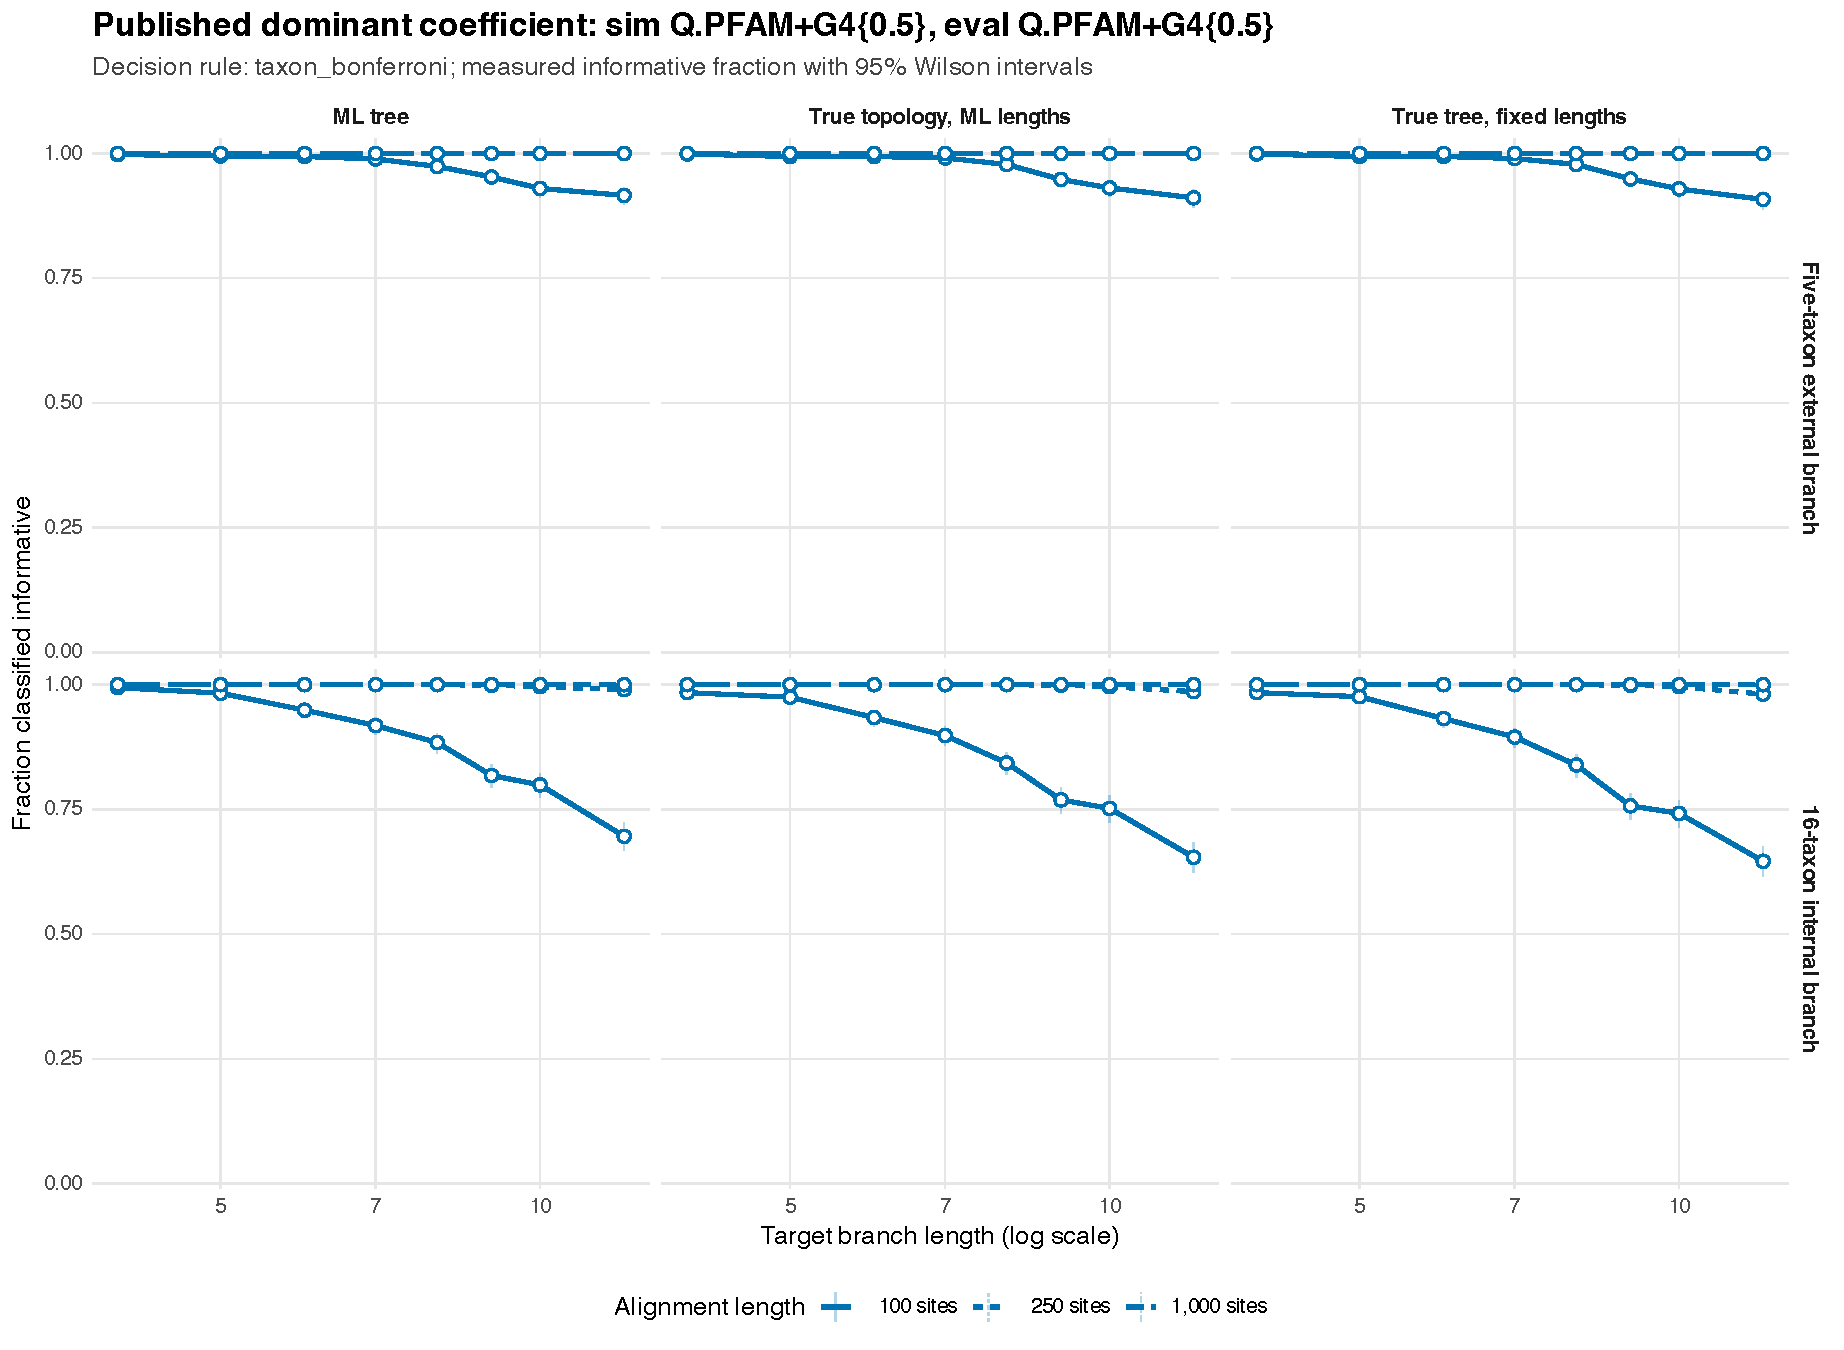
\includegraphics[width=0.49\textwidth]{figures/publication-suite/power/protein_Q_PFAM_G4_dominant.pdf}
  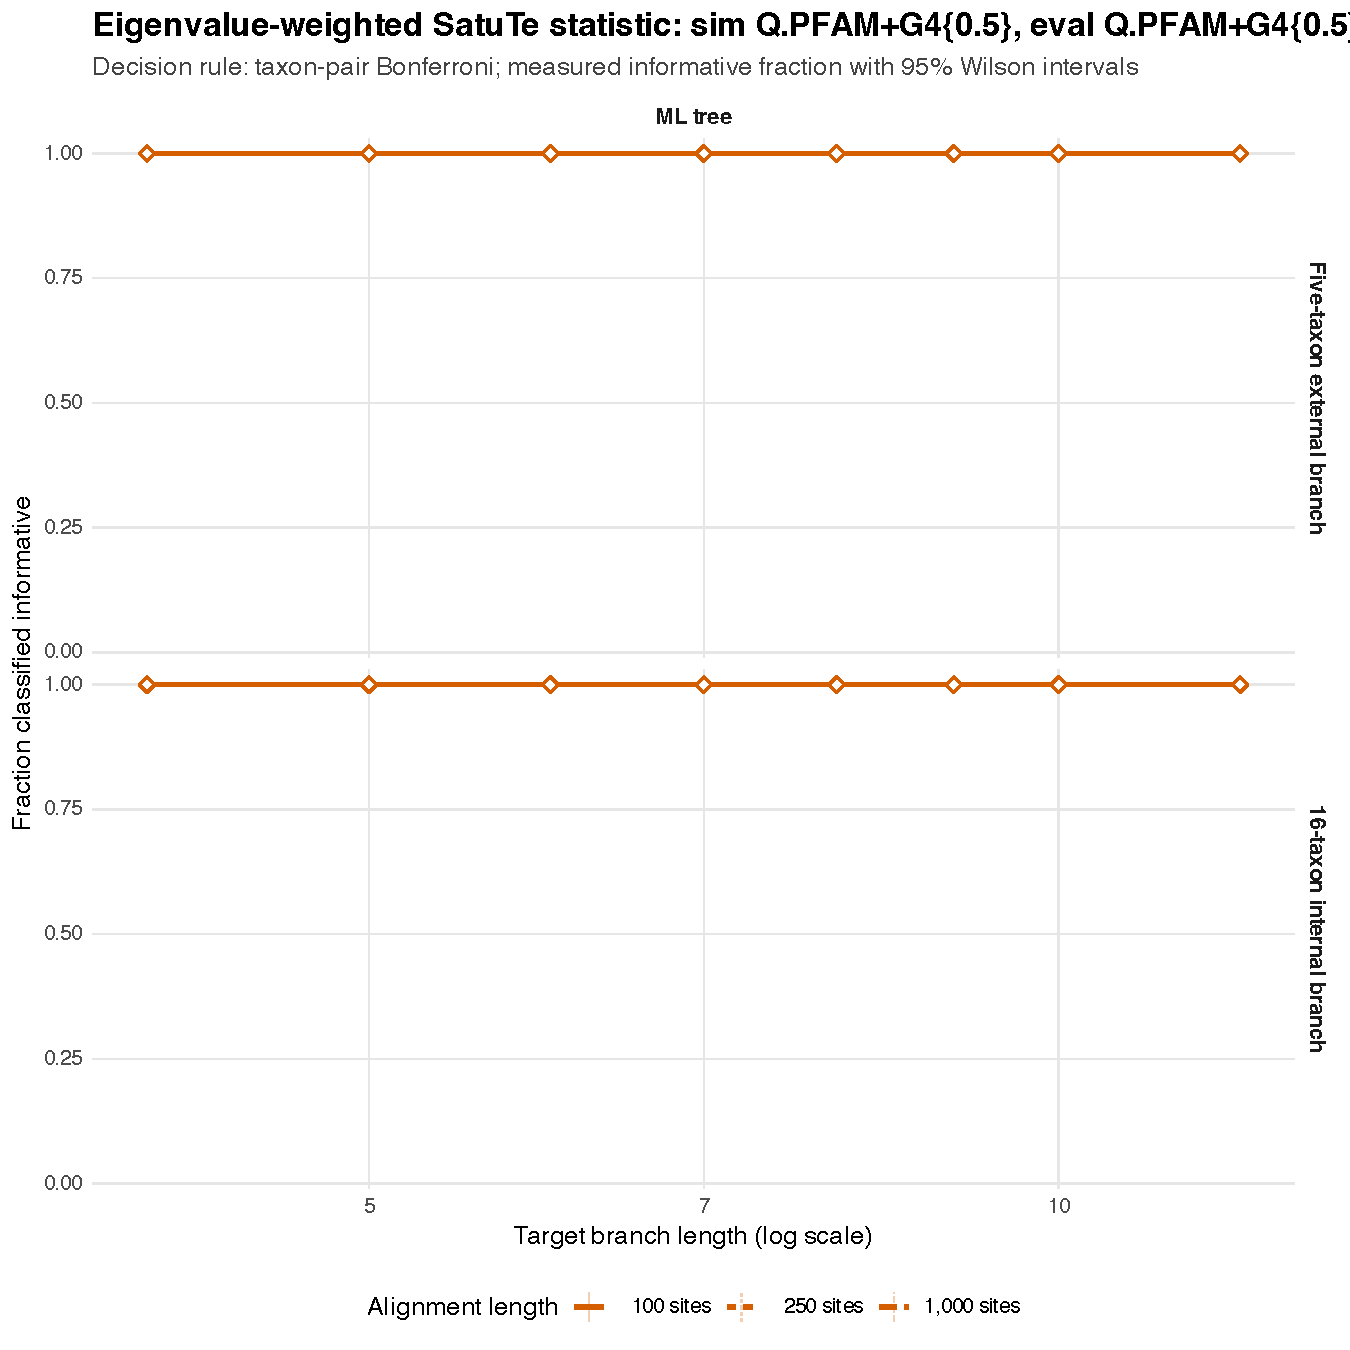
\includegraphics[width=0.49\textwidth]{figures/publication-suite/power/protein_Q_PFAM_G4_weighted.pdf}
  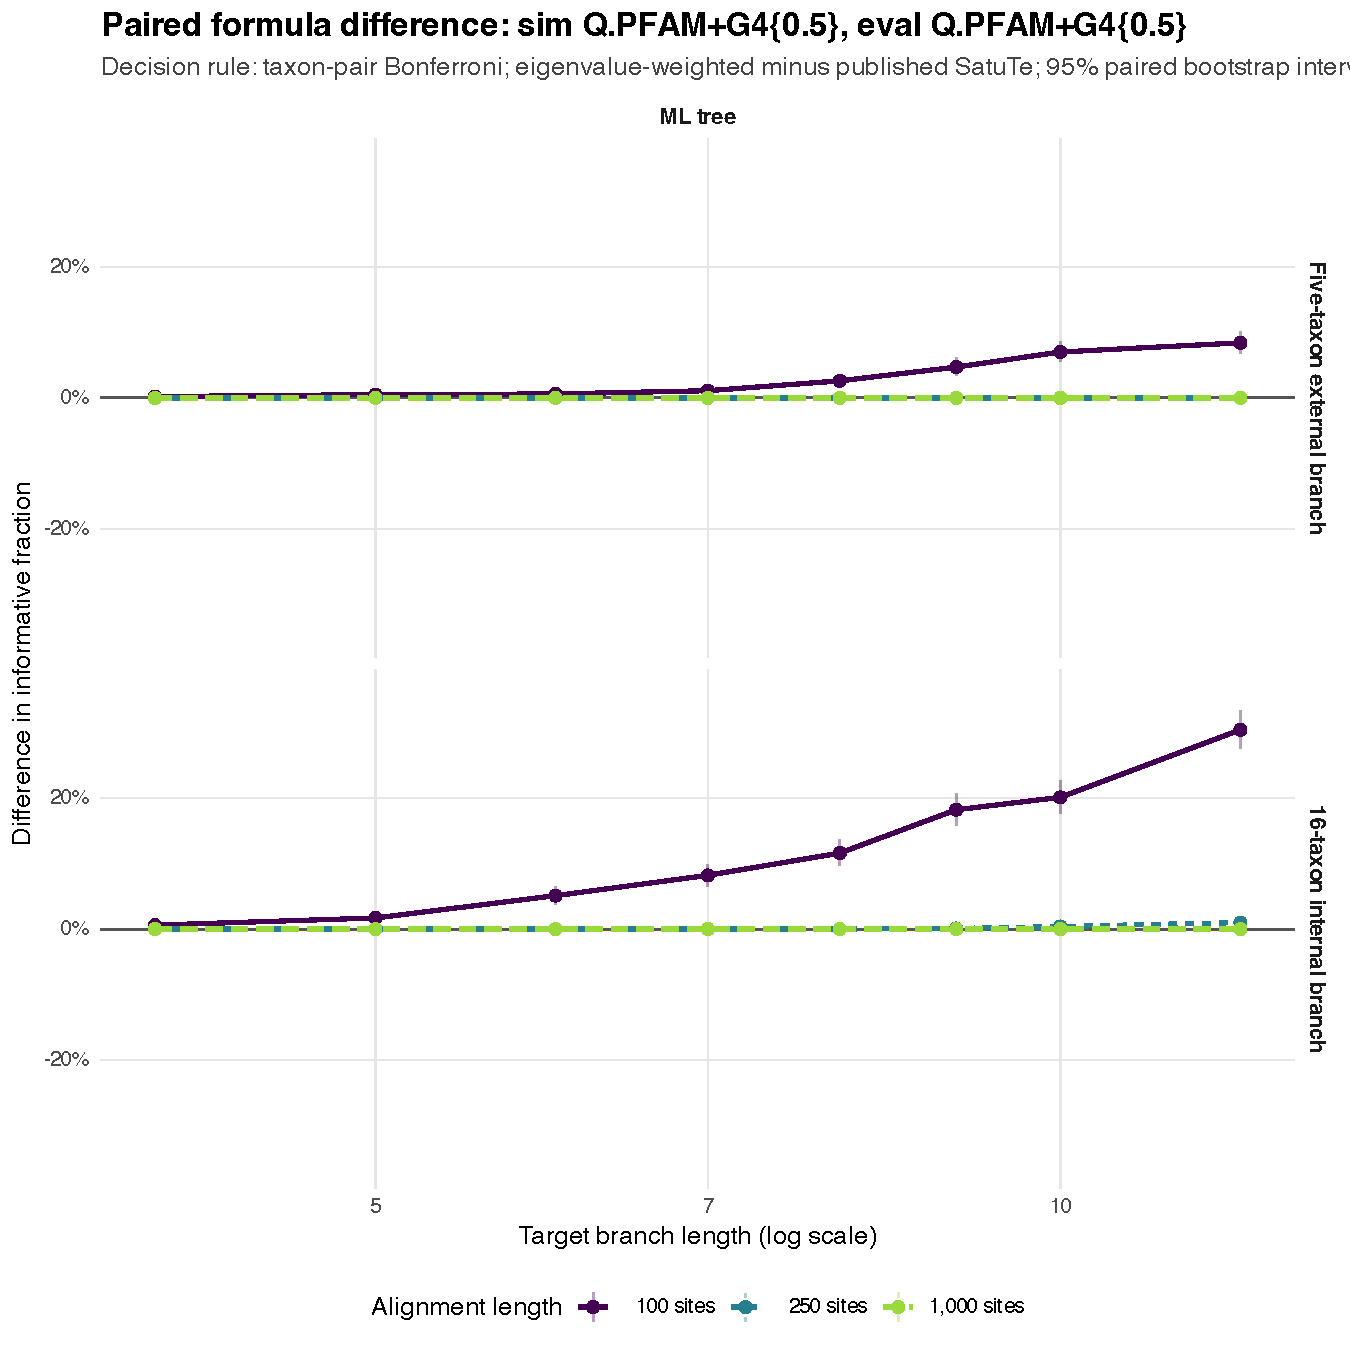
\includegraphics[width=0.72\textwidth]{figures/publication-suite/power/protein_Q_PFAM_G4_difference.pdf}
  \caption{\textbf{Matched Q.pfam+G4 power.} Dominant (top left), weighted (top right) and weighted-minus-dominant difference (bottom) under taxon Bonferroni. Weighting is never worse across the evaluated cells and gains up to 35.4 percentage points.}
  \makeatletter\cref@old@label{fig-supp-protein-qpfam}\makeatother
\end{figure}

\begin{figure}[p]
  \centering
  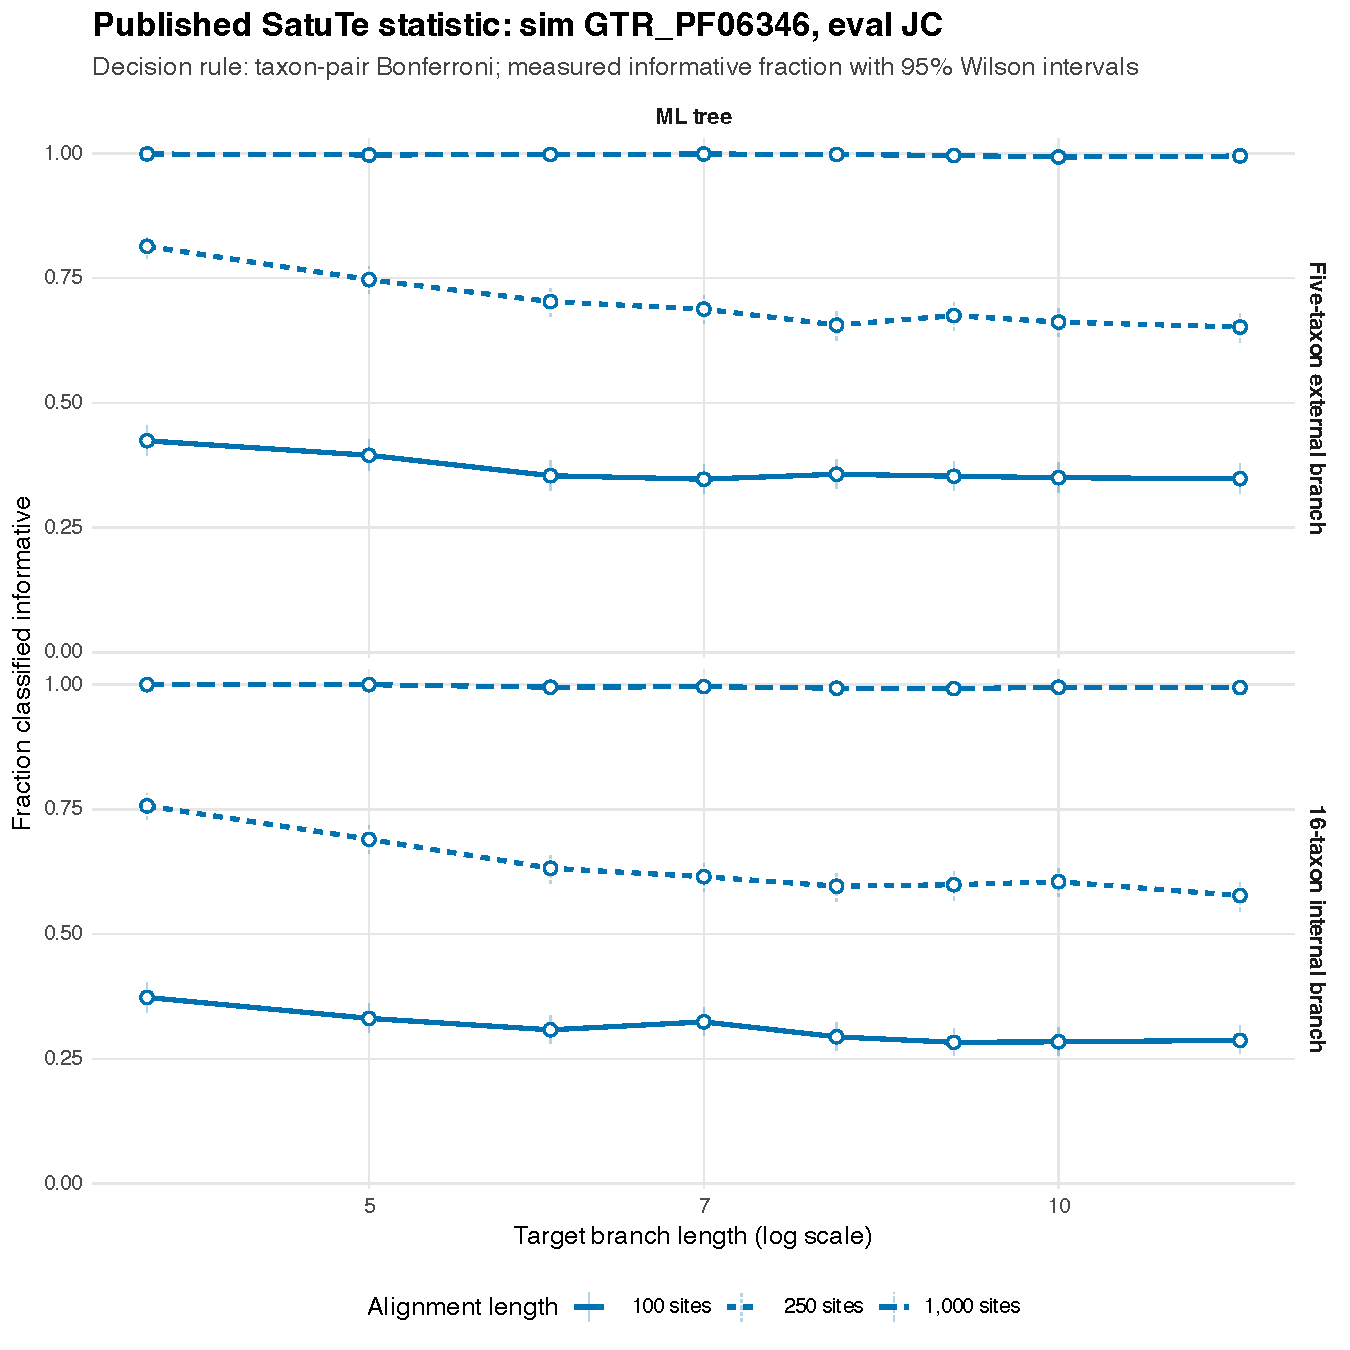
\includegraphics[width=0.49\textwidth]{figures/publication-suite/power/misspec_JC_dominant.pdf}
  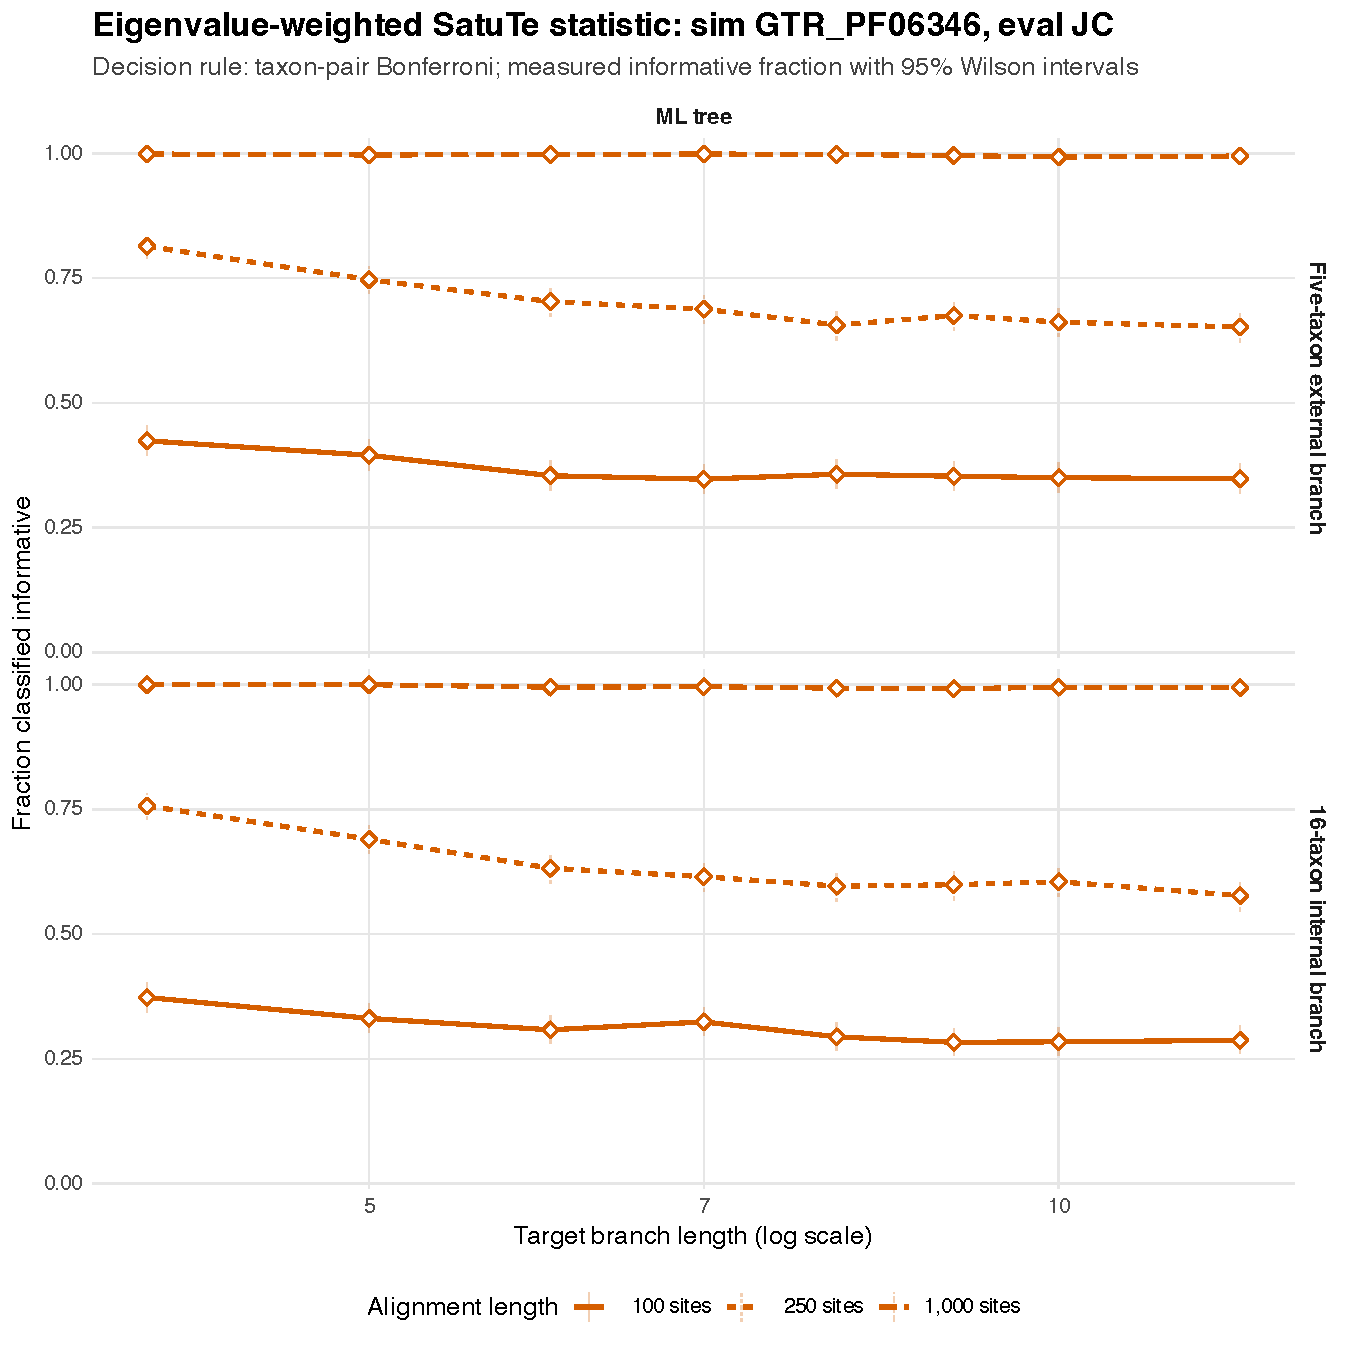
\includegraphics[width=0.49\textwidth]{figures/publication-suite/power/misspec_JC_weighted.pdf}
  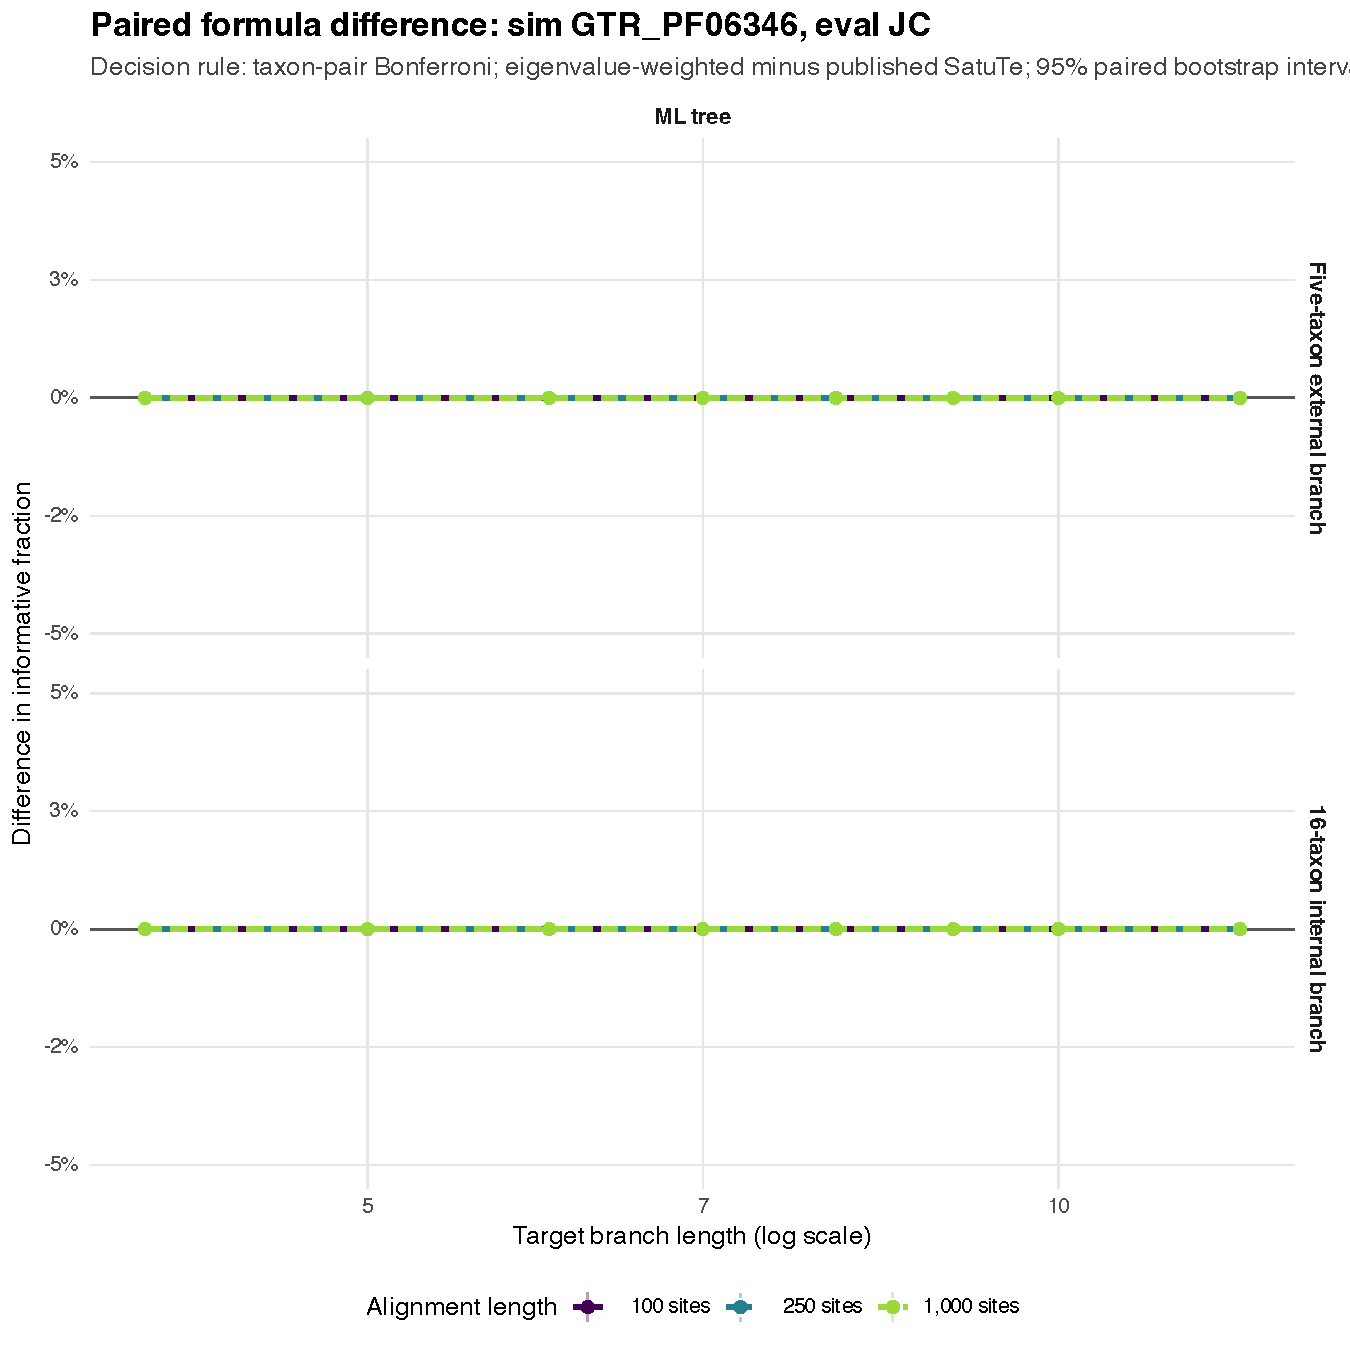
\includegraphics[width=0.72\textwidth]{figures/publication-suite/power/misspec_JC_difference.pdf}
  \caption{\textbf{GTR data evaluated by JC.} Dominant (top left), eigenvalue-weighted (top right) and paired difference (bottom) under taxon Bonferroni. The two formulas coincide under the JC evaluation model.}
  \makeatletter\cref@old@label{fig-supp-misspec-jc}\makeatother
\end{figure}

\begin{figure}[p]
  \centering
  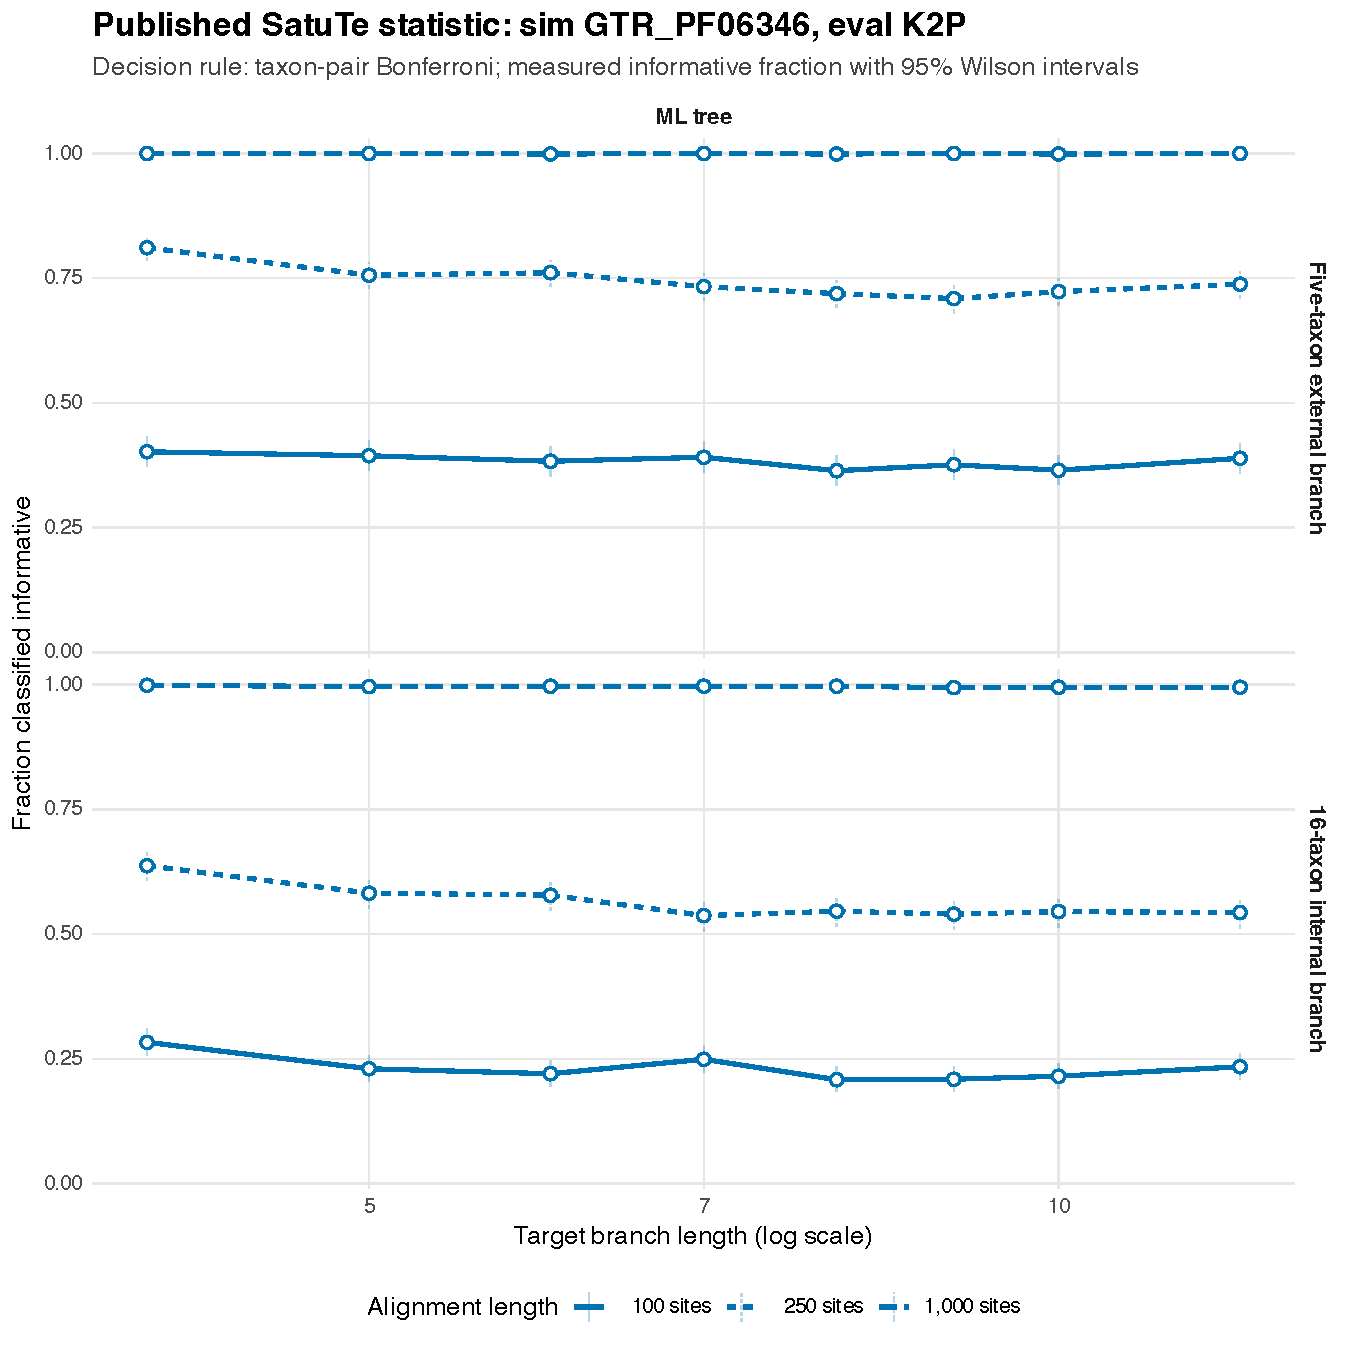
\includegraphics[width=0.49\textwidth]{figures/publication-suite/power/misspec_K2P_dominant.pdf}
  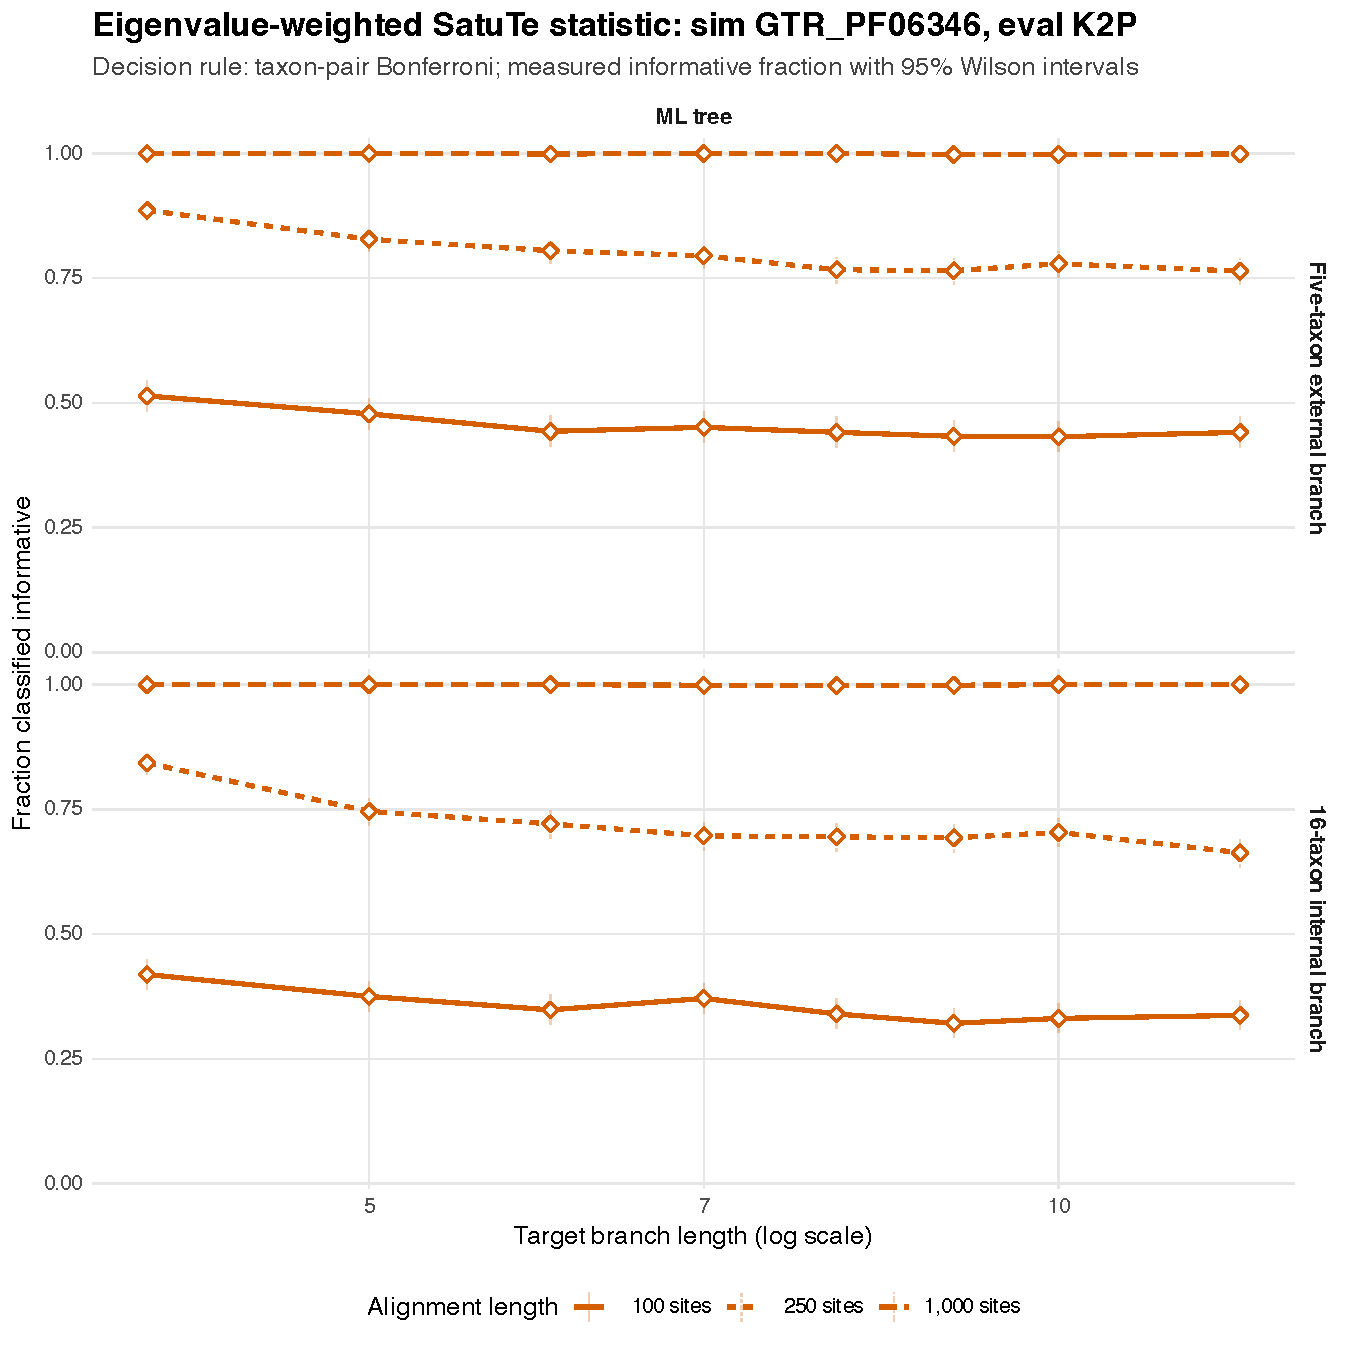
\includegraphics[width=0.49\textwidth]{figures/publication-suite/power/misspec_K2P_weighted.pdf}
  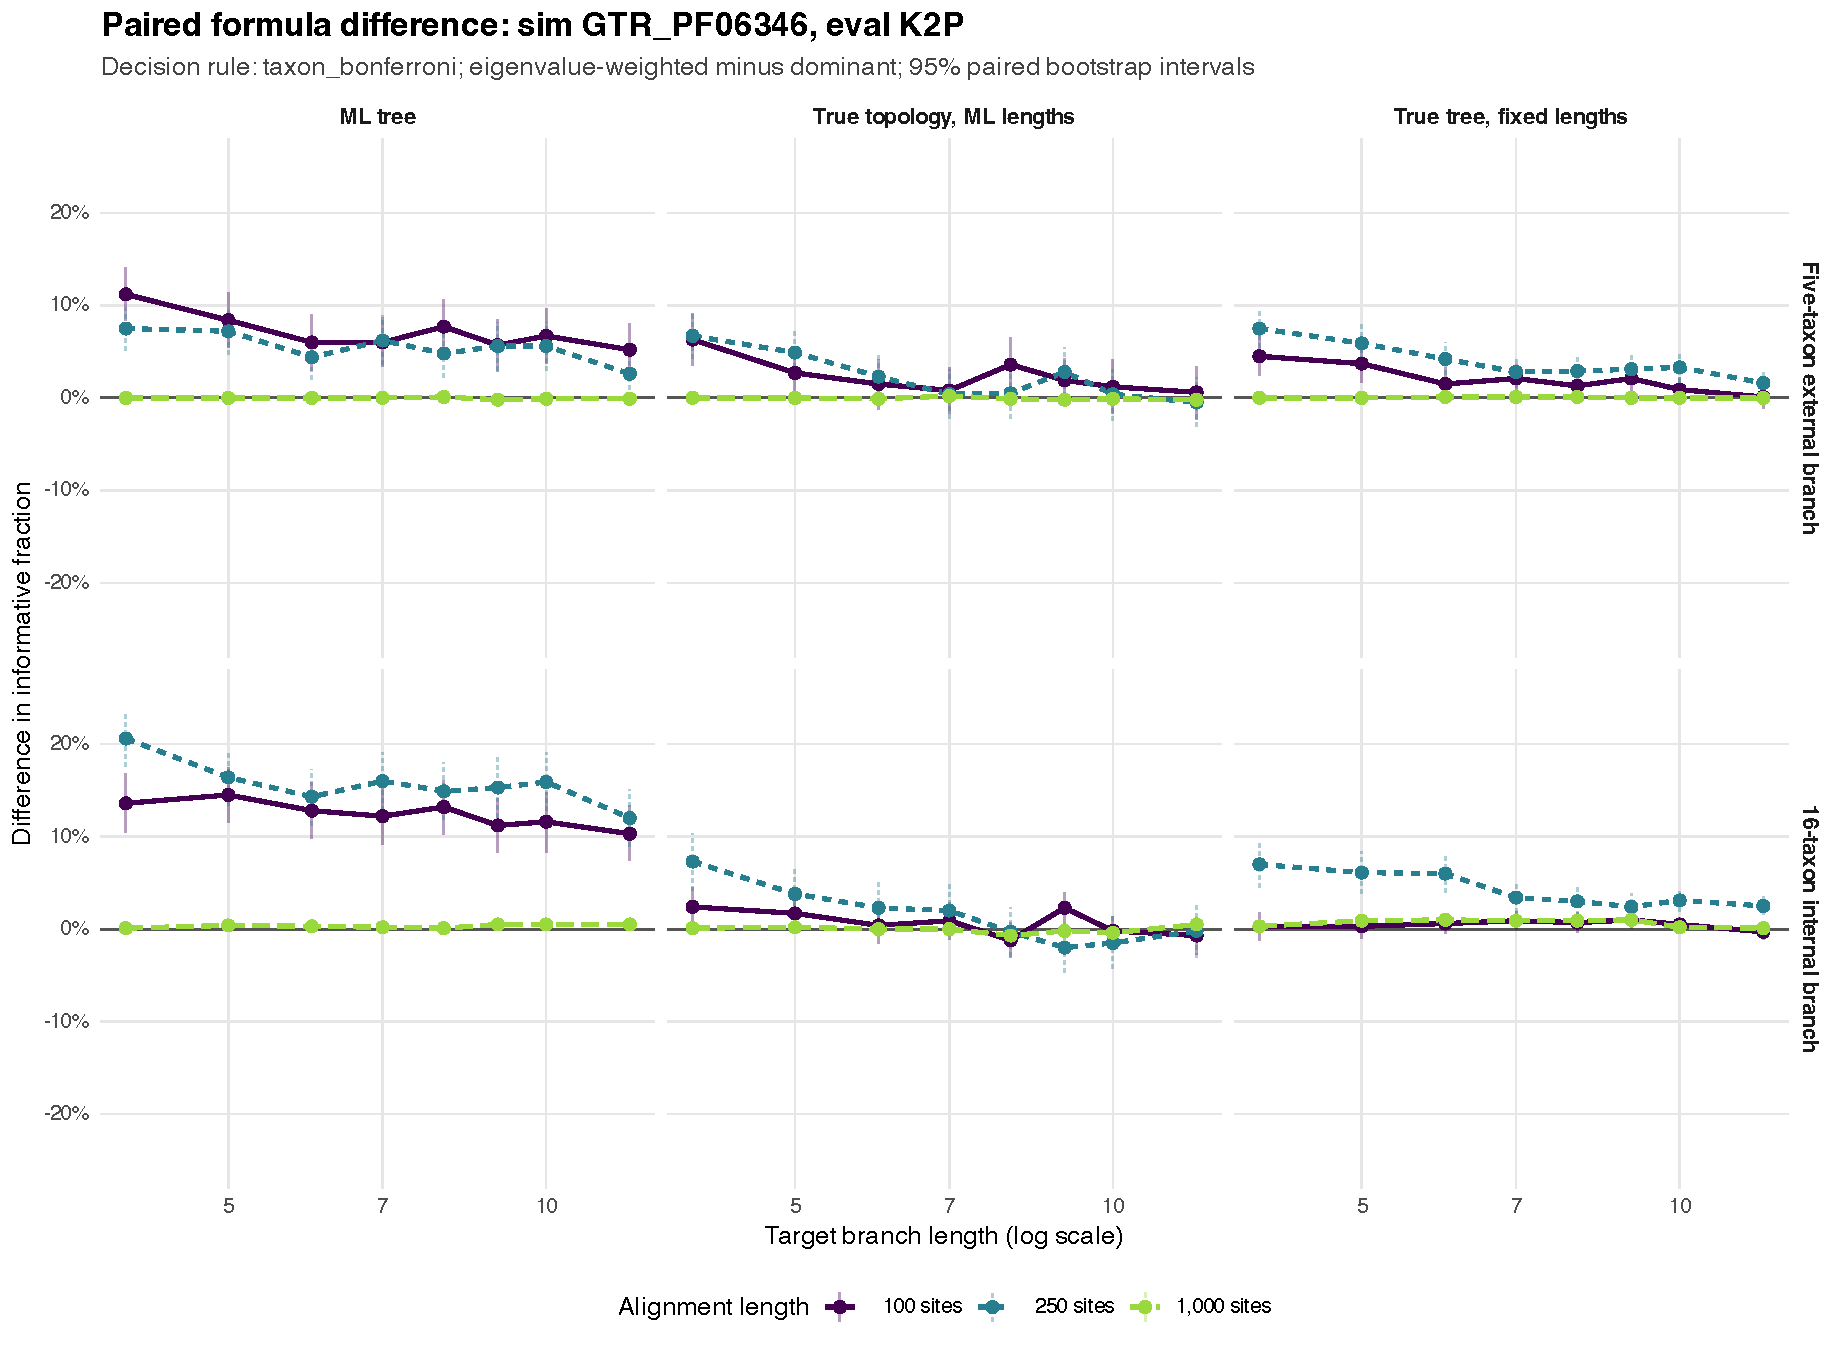
\includegraphics[width=0.72\textwidth]{figures/publication-suite/power/misspec_K2P_difference.pdf}
  \caption{\textbf{GTR data evaluated by K2P.} Dominant (top left), eigenvalue-weighted (top right) and paired difference (bottom) under taxon Bonferroni. Most cells favour weighting, although a minority show small negative differences.}
  \makeatletter\cref@old@label{fig-supp-misspec-k2p}\makeatother
\end{figure}

\begin{figure}[p]
  \centering
  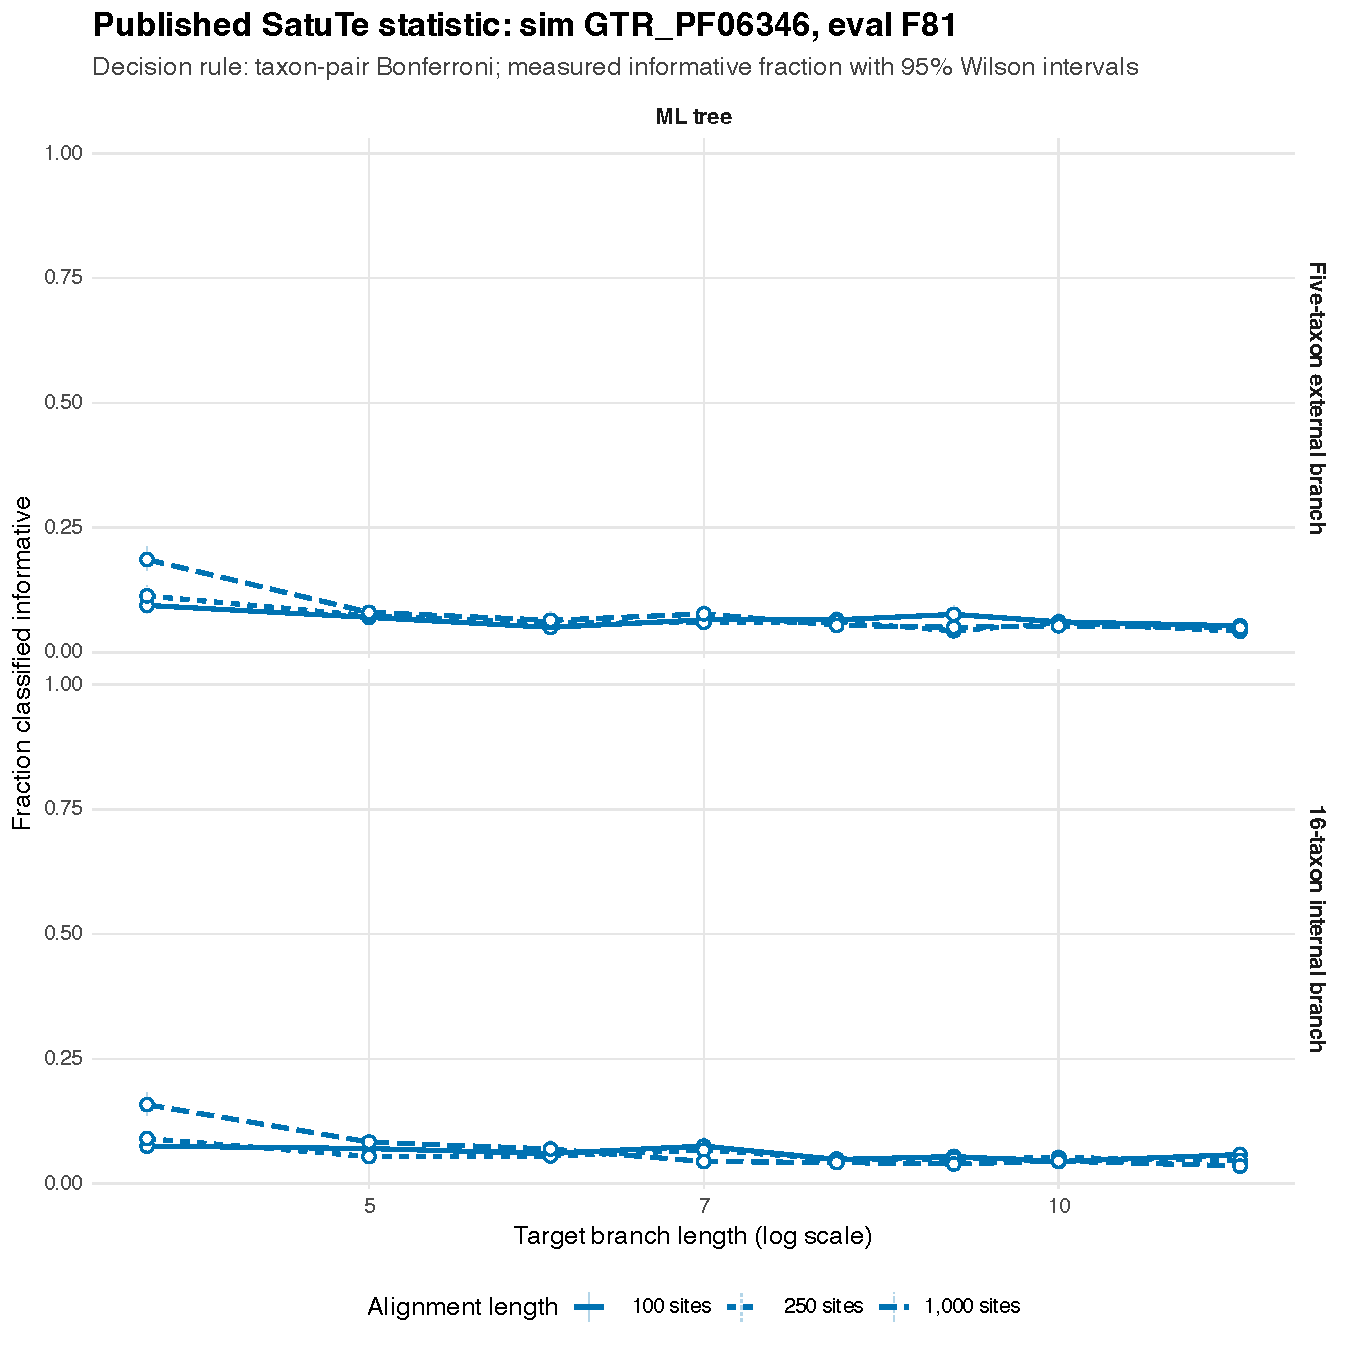
\includegraphics[width=0.49\textwidth]{figures/publication-suite/power/misspec_F81_dominant.pdf}
  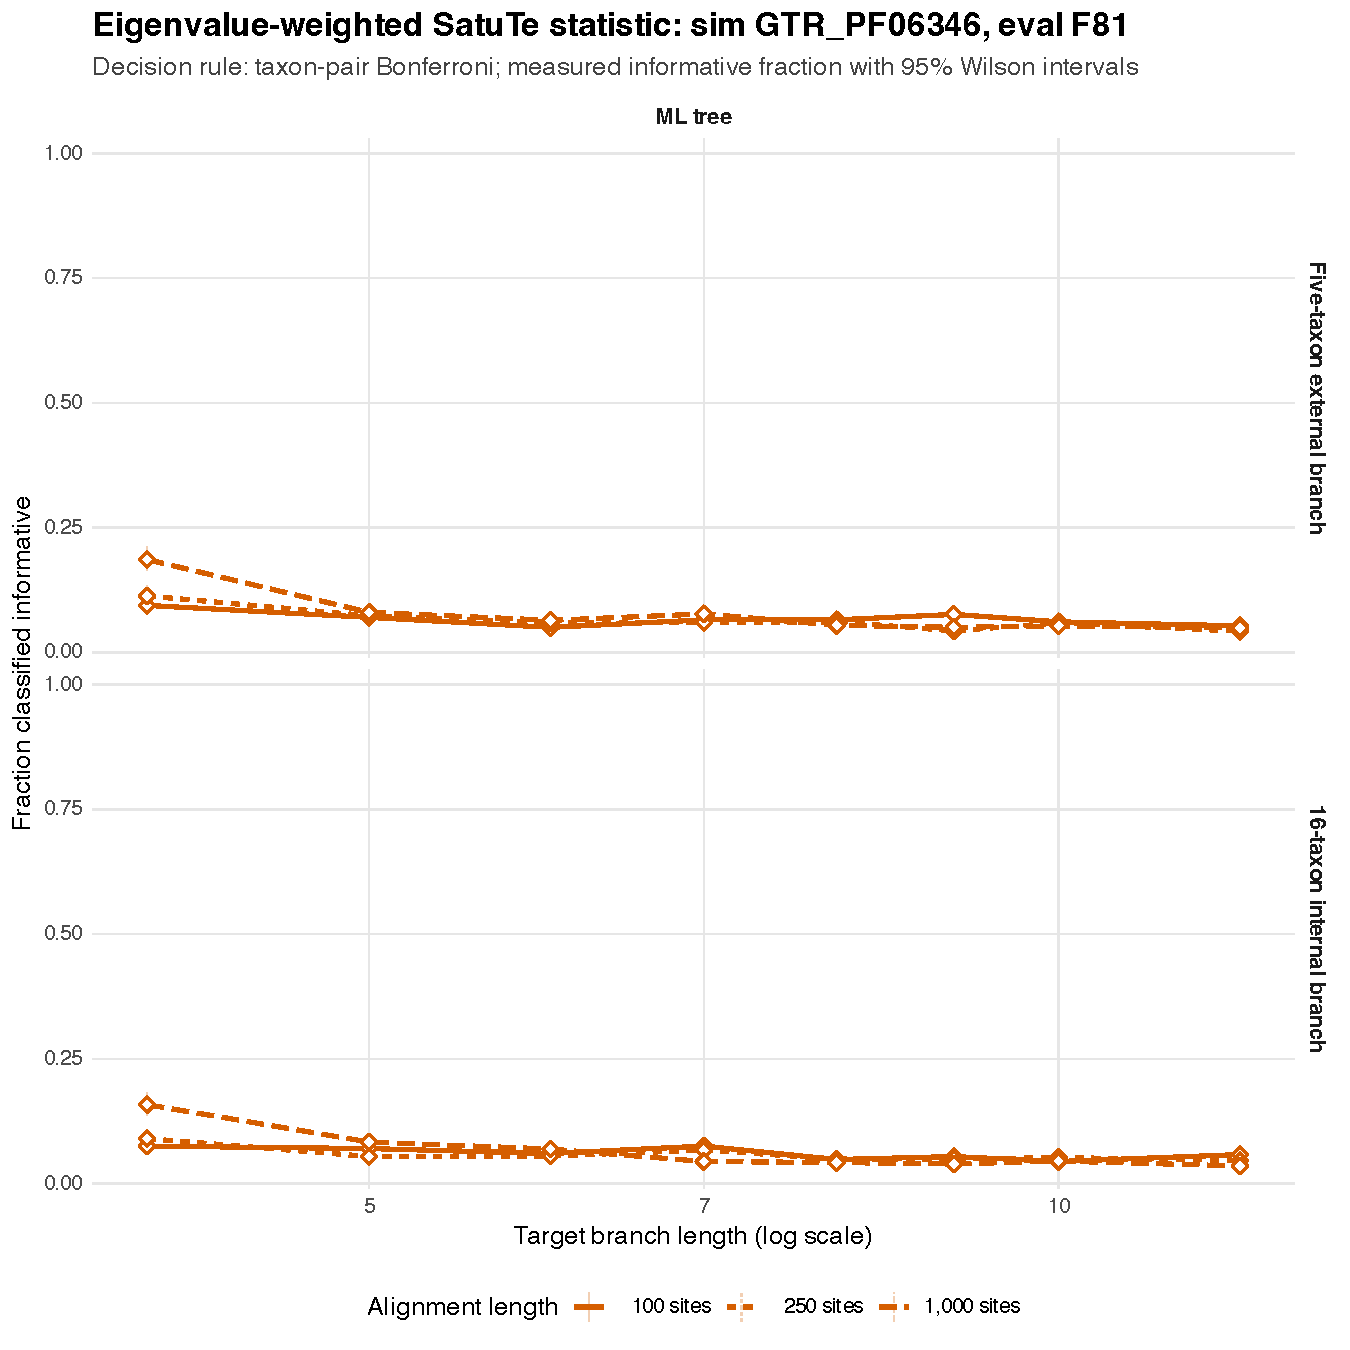
\includegraphics[width=0.49\textwidth]{figures/publication-suite/power/misspec_F81_weighted.pdf}
  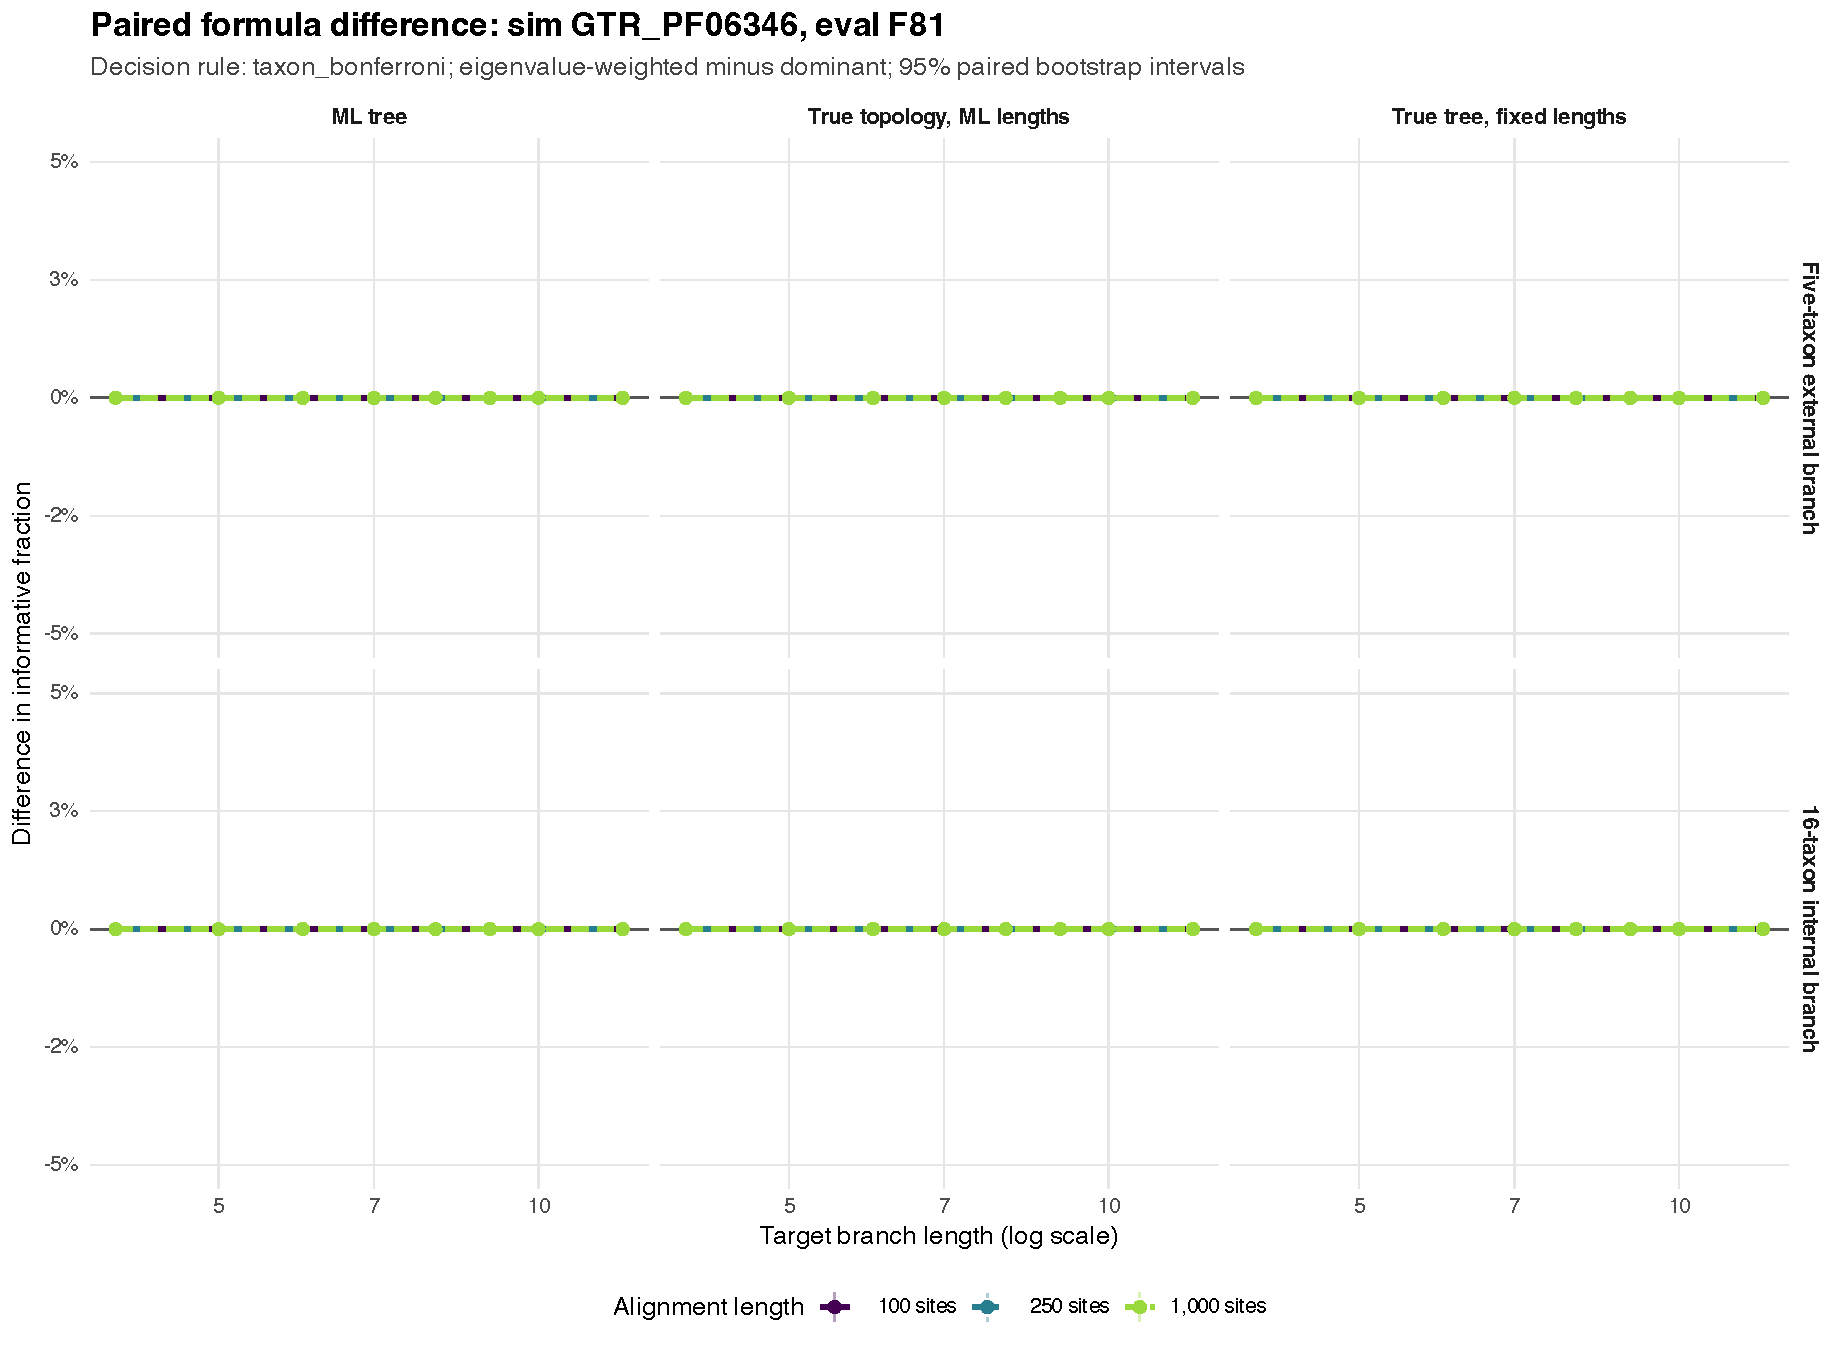
\includegraphics[width=0.72\textwidth]{figures/publication-suite/power/misspec_F81_difference.pdf}
  \caption{\textbf{GTR data evaluated by F81.} Dominant (top left), eigenvalue-weighted (top right) and paired difference (bottom) under taxon Bonferroni. The two formulas coincide under this evaluation model.}
  \makeatletter\cref@old@label{fig-supp-misspec-f81}\makeatother
\end{figure}

\clearpage

\begin{table}[p]
  \centering
  \small
  \begin{tabular}{lrrrr@{\qquad}lrrrr}
    \toprule
    Protein & Sites & 2D & 3D & \(\Delta Z\) & Protein & Sites & 2D & 3D & \(\Delta Z\) \\
    \midrule
    L2 & 317 & 11.68 & 11.65 & 0.03 & L18 & 141 & 8.23 & 8.11 & 0.12 \\
    L3 & 228 & 11.62 & 11.07 & 0.55 & L22 & 174 & 8.28 & 8.69 & -0.41 \\
    L4 & 245 & 11.06 & 11.02 & 0.04 & L24 & 81 & 7.77 & 7.68 & 0.09 \\
    L5 & 164 & 12.31 & 12.21 & 0.10 & S3 & 216 & 10.85 & 10.51 & 0.34 \\
    L6 & 220 & 10.34 & 10.27 & 0.07 & S8 & 141 & 10.03 & 9.77 & 0.26 \\
    L14 & 125 & 9.96 & 9.01 & 0.95 & S10 & 104 & 8.91 & 9.04 & -0.13 \\
    L15 & 122 & 7.72 & 8.75 & -1.03 & S17 & 74 & 7.92 & 7.37 & 0.55 \\
    L16 & 153 & 6.35 & 6.30 & 0.05 & S19 & 91 & 8.35 & 8.01 & 0.34 \\
    \bottomrule
  \end{tabular}
  \caption{\textbf{Per-protein topology comparison.} SatuTe \(Z\)-scores for the Eukaryota branch under the protein 2D tree and the rearranged 3D tree, with \(\Delta Z=Z_{2D}-Z_{3D}\). All proteins remain significant under both placements; L15, L22 and S10 favour the rearranged 3D placement.}
  \makeatletter\cref@old@label{tab-supp-protein-topology}\makeatother
\end{table}

\begin{table}[p]
  \centering
  \small
  \begin{tabular}{lrrrr}
    \toprule
    rRNA region & Alignment sites & 3D \(Z\) & Rearranged 2D \(Z\) & \(Z_{2D}-Z_{3D}\) \\
    \midrule
    R1 & 0--114 & 4.57 & 5.08 & 0.51 \\
    R2 & 115--431 & 6.13 & 5.94 & -0.19 \\
    R3 & 432--621 & 3.63 & 3.45 & -0.17 \\
    R4 & 622--1066 & 6.81 & 6.83 & 0.03 \\
    R5 & 1067--1221 & 8.99 & 8.93 & -0.06 \\
    R6 & 1222--1394 & 8.55 & 8.31 & -0.23 \\
    R7 & 1395--1565 & 8.93 & 8.35 & -0.59 \\
    R8 & 1566--1765 & 12.44 & 12.33 & -0.12 \\
    R9 & 1766--1946 & 9.33 & 9.65 & 0.33 \\
    \bottomrule
  \end{tabular}
  \caption{\textbf{rRNA-region topology comparison.} Six of nine regions have negative \(Z_{2D}-Z_{3D}\) and therefore a larger score under the 3D placement.}
  \makeatletter\cref@old@label{tab-supp-rrna-topology}\makeatother
\end{table}

\begin{table}[p]
  \centering
  \small
  \begin{tabular}{llrrrr}
    \toprule
    Partition & Branch & Windows & Dominant & Weighted & Weighted fraction \\
    \midrule
    Positions 1+2 & Genotype 1 & 507 & 1 & 1 & 0.2\% \\
     & Genotype 2 & 507 & 4 & 1 & 0.2\% \\
     & Genotype 3 & 507 & 5 & 1 & 0.2\% \\
    \addlinespace
    Position 3 & Genotype 1 & 252 & 11 & 6 & 2.4\% \\
     & Genotype 2 & 252 & 34 & 24 & 9.5\% \\
     & Genotype 3 & 252 & 33 & 27 & 10.7\% \\
    \bottomrule
  \end{tabular}
  \caption{\textbf{HCV saturated-window counts.} Counts use \(Z<z_{0.01}\) for three subtype-pair branches. Positions 1+2 and position 3 contain equal 36-site windows but span different genomic widths.}
  \makeatletter\cref@old@label{tab-supp-hcv-windows}\makeatother
\end{table}

\begin{figure}[p]
  \centering
  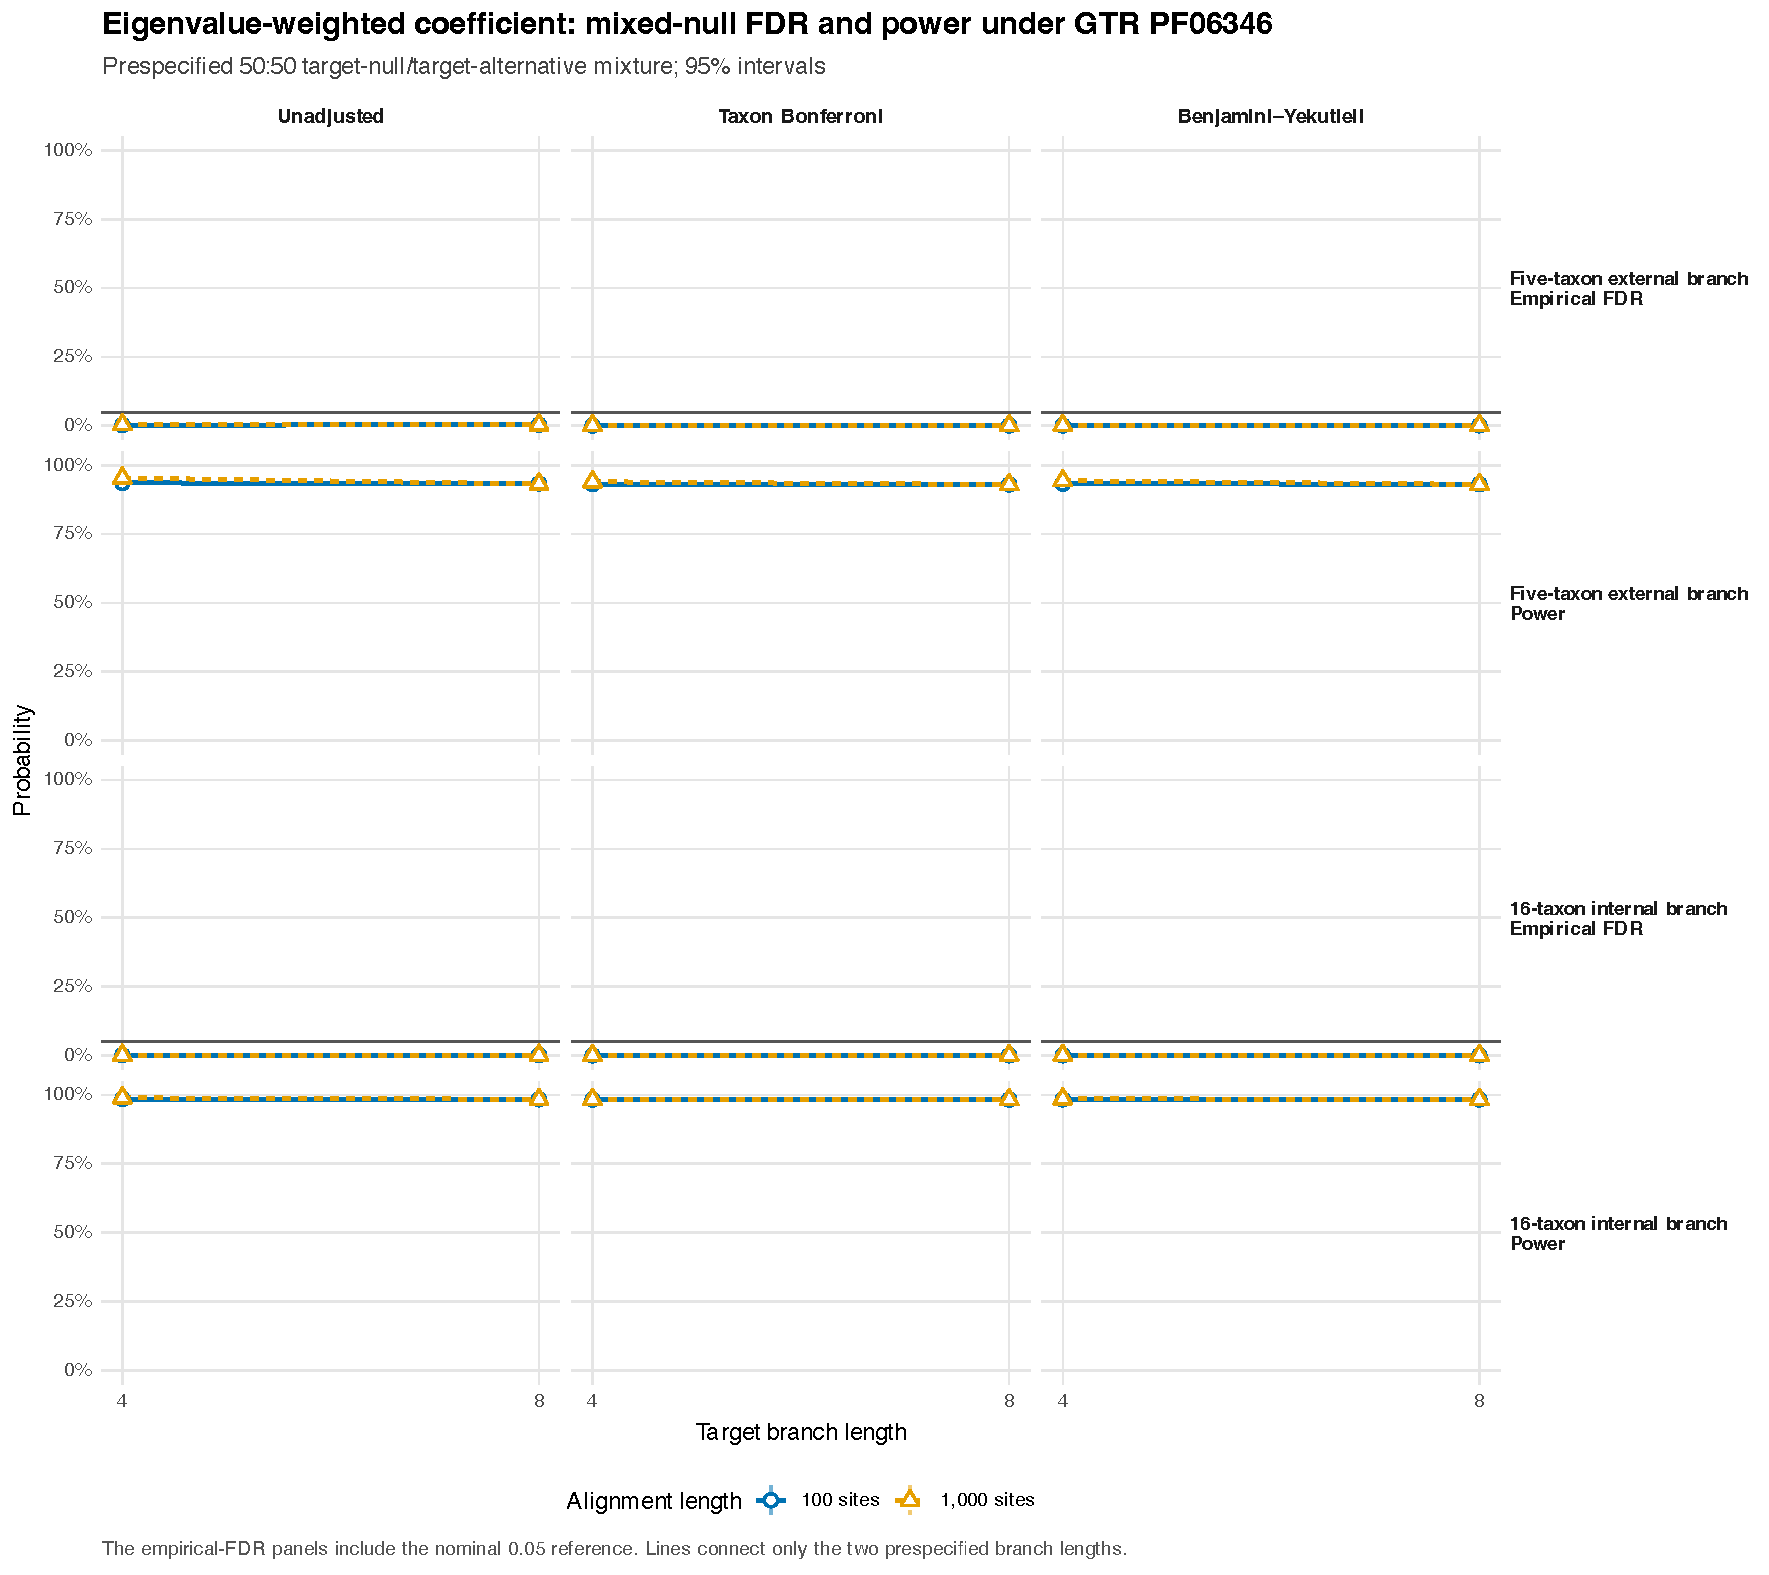
\includegraphics[width=0.48\textwidth]{figures/publication-suite/figure_fdr_weighted_power_2d_gtr.pdf}
  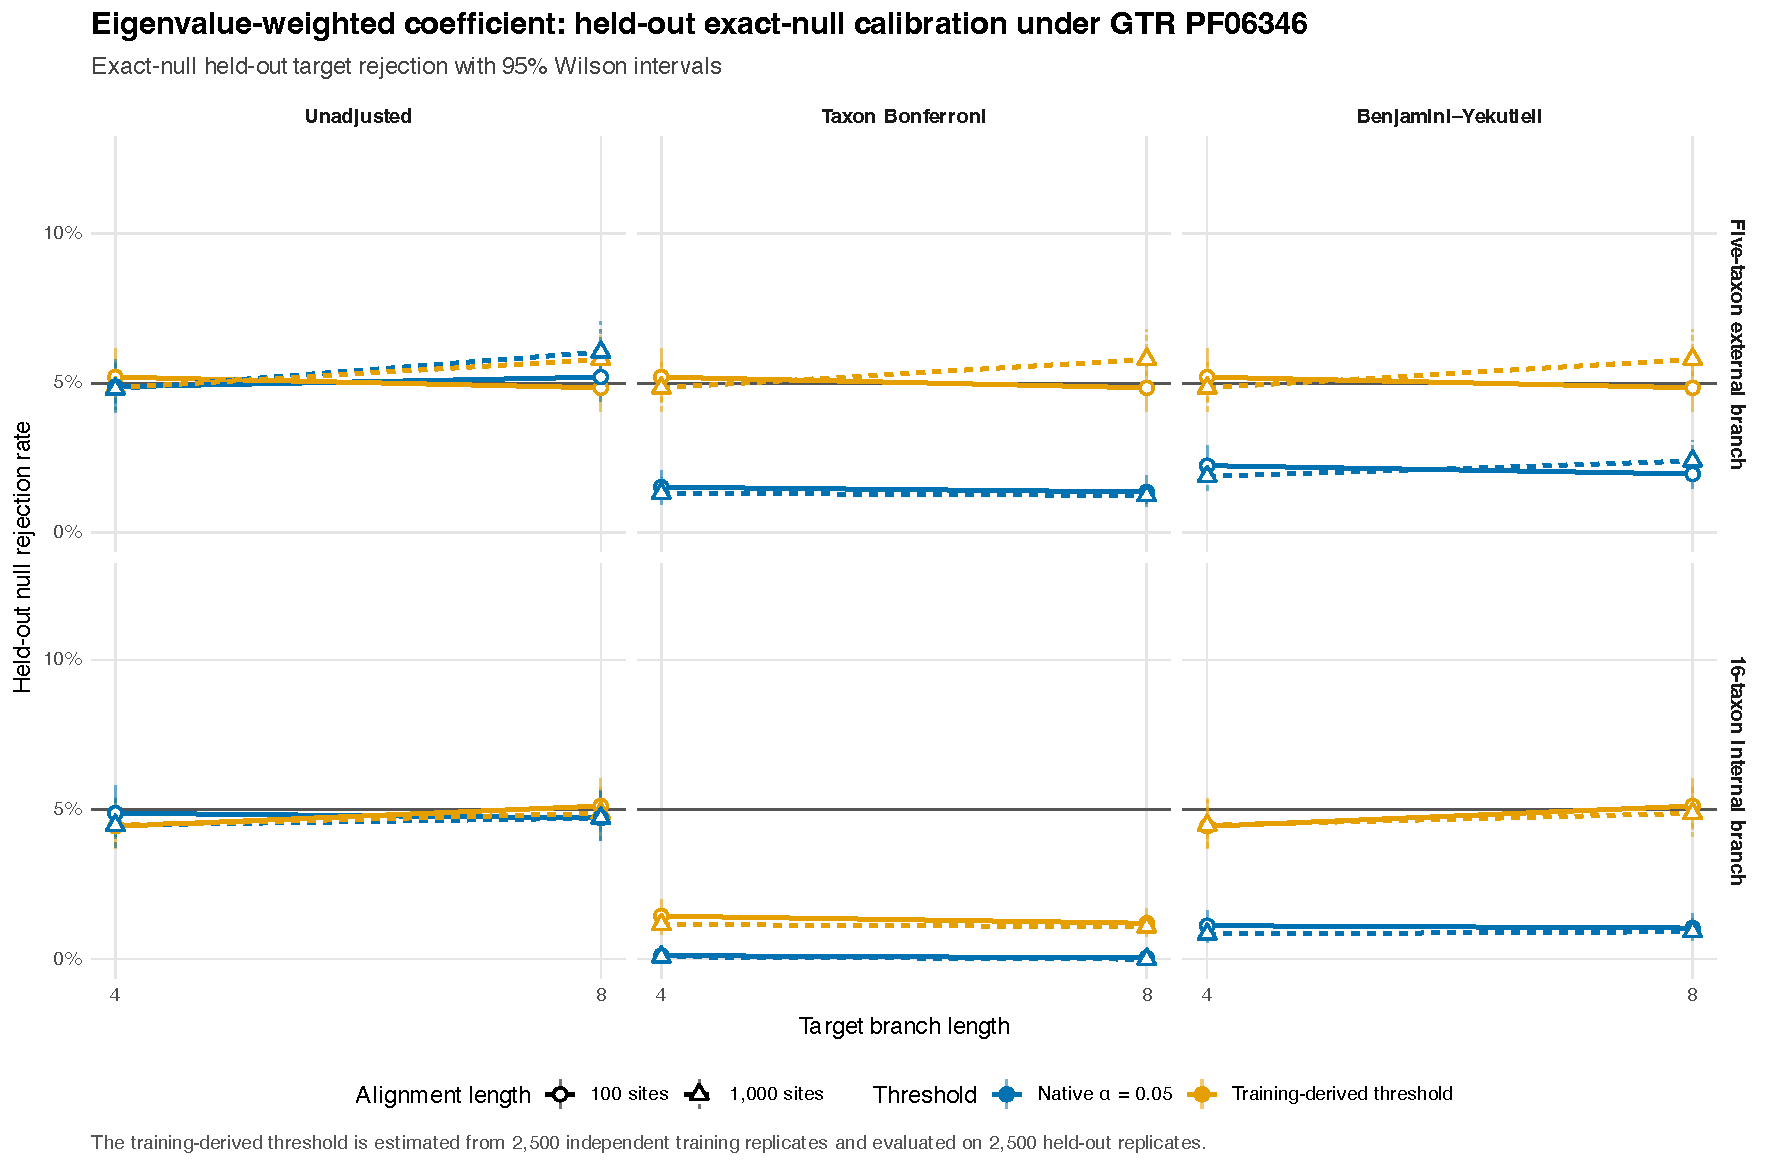
\includegraphics[width=0.48\textwidth]{figures/publication-suite/figure_fdr_weighted_null_calibration_2d_gtr.pdf}
  \caption{\textbf{Truth-labelled GTR calibration.} \textbf{a,} Empirical FDR and power of the weighted formula in a prespecified 50:50 mixed-null design. \textbf{b,} Native and training-derived rejection on 2,500 held-out exact nulls per cell. Columns show unadjusted, taxon-Bonferroni and BY rules.}
  \makeatletter\cref@old@label{fig-supp-fdr-gtr}\makeatother
\end{figure}

\clearpage
